
% Default to the notebook output style

    


% Inherit from the specified cell style.




    
\documentclass[11pt]{article}

    
    
    \usepackage[T1]{fontenc}
    % Nicer default font (+ math font) than Computer Modern for most use cases
    \usepackage{mathpazo}

    % Basic figure setup, for now with no caption control since it's done
    % automatically by Pandoc (which extracts ![](path) syntax from Markdown).
    \usepackage{graphicx}
    % We will generate all images so they have a width \maxwidth. This means
    % that they will get their normal width if they fit onto the page, but
    % are scaled down if they would overflow the margins.
    \makeatletter
    \def\maxwidth{\ifdim\Gin@nat@width>\linewidth\linewidth
    \else\Gin@nat@width\fi}
    \makeatother
    \let\Oldincludegraphics\includegraphics
    % Set max figure width to be 80% of text width, for now hardcoded.
    \renewcommand{\includegraphics}[1]{\Oldincludegraphics[width=.8\maxwidth]{#1}}
    % Ensure that by default, figures have no caption (until we provide a
    % proper Figure object with a Caption API and a way to capture that
    % in the conversion process - todo).
    \usepackage{caption}
    \DeclareCaptionLabelFormat{nolabel}{}
    \captionsetup{labelformat=nolabel}

    \usepackage{adjustbox} % Used to constrain images to a maximum size 
    \usepackage{xcolor} % Allow colors to be defined
    \usepackage{enumerate} % Needed for markdown enumerations to work
    \usepackage{geometry} % Used to adjust the document margins
    \usepackage{amsmath} % Equations
    \usepackage{amssymb} % Equations
    \usepackage{textcomp} % defines textquotesingle
    % Hack from http://tex.stackexchange.com/a/47451/13684:
    \AtBeginDocument{%
        \def\PYZsq{\textquotesingle}% Upright quotes in Pygmentized code
    }
    \usepackage{upquote} % Upright quotes for verbatim code
    \usepackage{eurosym} % defines \euro
    \usepackage[mathletters]{ucs} % Extended unicode (utf-8) support
    \usepackage[utf8x]{inputenc} % Allow utf-8 characters in the tex document
    \usepackage{fancyvrb} % verbatim replacement that allows latex
    \usepackage{grffile} % extends the file name processing of package graphics 
                         % to support a larger range 
    % The hyperref package gives us a pdf with properly built
    % internal navigation ('pdf bookmarks' for the table of contents,
    % internal cross-reference links, web links for URLs, etc.)
    \usepackage{hyperref}
    \usepackage{longtable} % longtable support required by pandoc >1.10
    \usepackage{booktabs}  % table support for pandoc > 1.12.2
    \usepackage[inline]{enumitem} % IRkernel/repr support (it uses the enumerate* environment)
    \usepackage[normalem]{ulem} % ulem is needed to support strikethroughs (\sout)
                                % normalem makes italics be italics, not underlines
    

    
    
    % Colors for the hyperref package
    \definecolor{urlcolor}{rgb}{0,.145,.698}
    \definecolor{linkcolor}{rgb}{.71,0.21,0.01}
    \definecolor{citecolor}{rgb}{.12,.54,.11}

    % ANSI colors
    \definecolor{ansi-black}{HTML}{3E424D}
    \definecolor{ansi-black-intense}{HTML}{282C36}
    \definecolor{ansi-red}{HTML}{E75C58}
    \definecolor{ansi-red-intense}{HTML}{B22B31}
    \definecolor{ansi-green}{HTML}{00A250}
    \definecolor{ansi-green-intense}{HTML}{007427}
    \definecolor{ansi-yellow}{HTML}{DDB62B}
    \definecolor{ansi-yellow-intense}{HTML}{B27D12}
    \definecolor{ansi-blue}{HTML}{208FFB}
    \definecolor{ansi-blue-intense}{HTML}{0065CA}
    \definecolor{ansi-magenta}{HTML}{D160C4}
    \definecolor{ansi-magenta-intense}{HTML}{A03196}
    \definecolor{ansi-cyan}{HTML}{60C6C8}
    \definecolor{ansi-cyan-intense}{HTML}{258F8F}
    \definecolor{ansi-white}{HTML}{C5C1B4}
    \definecolor{ansi-white-intense}{HTML}{A1A6B2}

    % commands and environments needed by pandoc snippets
    % extracted from the output of `pandoc -s`
    \providecommand{\tightlist}{%
      \setlength{\itemsep}{0pt}\setlength{\parskip}{0pt}}
    \DefineVerbatimEnvironment{Highlighting}{Verbatim}{commandchars=\\\{\}}
    % Add ',fontsize=\small' for more characters per line
    \newenvironment{Shaded}{}{}
    \newcommand{\KeywordTok}[1]{\textcolor[rgb]{0.00,0.44,0.13}{\textbf{{#1}}}}
    \newcommand{\DataTypeTok}[1]{\textcolor[rgb]{0.56,0.13,0.00}{{#1}}}
    \newcommand{\DecValTok}[1]{\textcolor[rgb]{0.25,0.63,0.44}{{#1}}}
    \newcommand{\BaseNTok}[1]{\textcolor[rgb]{0.25,0.63,0.44}{{#1}}}
    \newcommand{\FloatTok}[1]{\textcolor[rgb]{0.25,0.63,0.44}{{#1}}}
    \newcommand{\CharTok}[1]{\textcolor[rgb]{0.25,0.44,0.63}{{#1}}}
    \newcommand{\StringTok}[1]{\textcolor[rgb]{0.25,0.44,0.63}{{#1}}}
    \newcommand{\CommentTok}[1]{\textcolor[rgb]{0.38,0.63,0.69}{\textit{{#1}}}}
    \newcommand{\OtherTok}[1]{\textcolor[rgb]{0.00,0.44,0.13}{{#1}}}
    \newcommand{\AlertTok}[1]{\textcolor[rgb]{1.00,0.00,0.00}{\textbf{{#1}}}}
    \newcommand{\FunctionTok}[1]{\textcolor[rgb]{0.02,0.16,0.49}{{#1}}}
    \newcommand{\RegionMarkerTok}[1]{{#1}}
    \newcommand{\ErrorTok}[1]{\textcolor[rgb]{1.00,0.00,0.00}{\textbf{{#1}}}}
    \newcommand{\NormalTok}[1]{{#1}}
    
    % Additional commands for more recent versions of Pandoc
    \newcommand{\ConstantTok}[1]{\textcolor[rgb]{0.53,0.00,0.00}{{#1}}}
    \newcommand{\SpecialCharTok}[1]{\textcolor[rgb]{0.25,0.44,0.63}{{#1}}}
    \newcommand{\VerbatimStringTok}[1]{\textcolor[rgb]{0.25,0.44,0.63}{{#1}}}
    \newcommand{\SpecialStringTok}[1]{\textcolor[rgb]{0.73,0.40,0.53}{{#1}}}
    \newcommand{\ImportTok}[1]{{#1}}
    \newcommand{\DocumentationTok}[1]{\textcolor[rgb]{0.73,0.13,0.13}{\textit{{#1}}}}
    \newcommand{\AnnotationTok}[1]{\textcolor[rgb]{0.38,0.63,0.69}{\textbf{\textit{{#1}}}}}
    \newcommand{\CommentVarTok}[1]{\textcolor[rgb]{0.38,0.63,0.69}{\textbf{\textit{{#1}}}}}
    \newcommand{\VariableTok}[1]{\textcolor[rgb]{0.10,0.09,0.49}{{#1}}}
    \newcommand{\ControlFlowTok}[1]{\textcolor[rgb]{0.00,0.44,0.13}{\textbf{{#1}}}}
    \newcommand{\OperatorTok}[1]{\textcolor[rgb]{0.40,0.40,0.40}{{#1}}}
    \newcommand{\BuiltInTok}[1]{{#1}}
    \newcommand{\ExtensionTok}[1]{{#1}}
    \newcommand{\PreprocessorTok}[1]{\textcolor[rgb]{0.74,0.48,0.00}{{#1}}}
    \newcommand{\AttributeTok}[1]{\textcolor[rgb]{0.49,0.56,0.16}{{#1}}}
    \newcommand{\InformationTok}[1]{\textcolor[rgb]{0.38,0.63,0.69}{\textbf{\textit{{#1}}}}}
    \newcommand{\WarningTok}[1]{\textcolor[rgb]{0.38,0.63,0.69}{\textbf{\textit{{#1}}}}}
    
    
    % Define a nice break command that doesn't care if a line doesn't already
    % exist.
    \def\br{\hspace*{\fill} \\* }
    % Math Jax compatability definitions
    \def\gt{>}
    \def\lt{<}
    % Document parameters
    \title{Assignment3}
    
    
    

    % Pygments definitions
    
\makeatletter
\def\PY@reset{\let\PY@it=\relax \let\PY@bf=\relax%
    \let\PY@ul=\relax \let\PY@tc=\relax%
    \let\PY@bc=\relax \let\PY@ff=\relax}
\def\PY@tok#1{\csname PY@tok@#1\endcsname}
\def\PY@toks#1+{\ifx\relax#1\empty\else%
    \PY@tok{#1}\expandafter\PY@toks\fi}
\def\PY@do#1{\PY@bc{\PY@tc{\PY@ul{%
    \PY@it{\PY@bf{\PY@ff{#1}}}}}}}
\def\PY#1#2{\PY@reset\PY@toks#1+\relax+\PY@do{#2}}

\expandafter\def\csname PY@tok@w\endcsname{\def\PY@tc##1{\textcolor[rgb]{0.73,0.73,0.73}{##1}}}
\expandafter\def\csname PY@tok@c\endcsname{\let\PY@it=\textit\def\PY@tc##1{\textcolor[rgb]{0.25,0.50,0.50}{##1}}}
\expandafter\def\csname PY@tok@cp\endcsname{\def\PY@tc##1{\textcolor[rgb]{0.74,0.48,0.00}{##1}}}
\expandafter\def\csname PY@tok@k\endcsname{\let\PY@bf=\textbf\def\PY@tc##1{\textcolor[rgb]{0.00,0.50,0.00}{##1}}}
\expandafter\def\csname PY@tok@kp\endcsname{\def\PY@tc##1{\textcolor[rgb]{0.00,0.50,0.00}{##1}}}
\expandafter\def\csname PY@tok@kt\endcsname{\def\PY@tc##1{\textcolor[rgb]{0.69,0.00,0.25}{##1}}}
\expandafter\def\csname PY@tok@o\endcsname{\def\PY@tc##1{\textcolor[rgb]{0.40,0.40,0.40}{##1}}}
\expandafter\def\csname PY@tok@ow\endcsname{\let\PY@bf=\textbf\def\PY@tc##1{\textcolor[rgb]{0.67,0.13,1.00}{##1}}}
\expandafter\def\csname PY@tok@nb\endcsname{\def\PY@tc##1{\textcolor[rgb]{0.00,0.50,0.00}{##1}}}
\expandafter\def\csname PY@tok@nf\endcsname{\def\PY@tc##1{\textcolor[rgb]{0.00,0.00,1.00}{##1}}}
\expandafter\def\csname PY@tok@nc\endcsname{\let\PY@bf=\textbf\def\PY@tc##1{\textcolor[rgb]{0.00,0.00,1.00}{##1}}}
\expandafter\def\csname PY@tok@nn\endcsname{\let\PY@bf=\textbf\def\PY@tc##1{\textcolor[rgb]{0.00,0.00,1.00}{##1}}}
\expandafter\def\csname PY@tok@ne\endcsname{\let\PY@bf=\textbf\def\PY@tc##1{\textcolor[rgb]{0.82,0.25,0.23}{##1}}}
\expandafter\def\csname PY@tok@nv\endcsname{\def\PY@tc##1{\textcolor[rgb]{0.10,0.09,0.49}{##1}}}
\expandafter\def\csname PY@tok@no\endcsname{\def\PY@tc##1{\textcolor[rgb]{0.53,0.00,0.00}{##1}}}
\expandafter\def\csname PY@tok@nl\endcsname{\def\PY@tc##1{\textcolor[rgb]{0.63,0.63,0.00}{##1}}}
\expandafter\def\csname PY@tok@ni\endcsname{\let\PY@bf=\textbf\def\PY@tc##1{\textcolor[rgb]{0.60,0.60,0.60}{##1}}}
\expandafter\def\csname PY@tok@na\endcsname{\def\PY@tc##1{\textcolor[rgb]{0.49,0.56,0.16}{##1}}}
\expandafter\def\csname PY@tok@nt\endcsname{\let\PY@bf=\textbf\def\PY@tc##1{\textcolor[rgb]{0.00,0.50,0.00}{##1}}}
\expandafter\def\csname PY@tok@nd\endcsname{\def\PY@tc##1{\textcolor[rgb]{0.67,0.13,1.00}{##1}}}
\expandafter\def\csname PY@tok@s\endcsname{\def\PY@tc##1{\textcolor[rgb]{0.73,0.13,0.13}{##1}}}
\expandafter\def\csname PY@tok@sd\endcsname{\let\PY@it=\textit\def\PY@tc##1{\textcolor[rgb]{0.73,0.13,0.13}{##1}}}
\expandafter\def\csname PY@tok@si\endcsname{\let\PY@bf=\textbf\def\PY@tc##1{\textcolor[rgb]{0.73,0.40,0.53}{##1}}}
\expandafter\def\csname PY@tok@se\endcsname{\let\PY@bf=\textbf\def\PY@tc##1{\textcolor[rgb]{0.73,0.40,0.13}{##1}}}
\expandafter\def\csname PY@tok@sr\endcsname{\def\PY@tc##1{\textcolor[rgb]{0.73,0.40,0.53}{##1}}}
\expandafter\def\csname PY@tok@ss\endcsname{\def\PY@tc##1{\textcolor[rgb]{0.10,0.09,0.49}{##1}}}
\expandafter\def\csname PY@tok@sx\endcsname{\def\PY@tc##1{\textcolor[rgb]{0.00,0.50,0.00}{##1}}}
\expandafter\def\csname PY@tok@m\endcsname{\def\PY@tc##1{\textcolor[rgb]{0.40,0.40,0.40}{##1}}}
\expandafter\def\csname PY@tok@gh\endcsname{\let\PY@bf=\textbf\def\PY@tc##1{\textcolor[rgb]{0.00,0.00,0.50}{##1}}}
\expandafter\def\csname PY@tok@gu\endcsname{\let\PY@bf=\textbf\def\PY@tc##1{\textcolor[rgb]{0.50,0.00,0.50}{##1}}}
\expandafter\def\csname PY@tok@gd\endcsname{\def\PY@tc##1{\textcolor[rgb]{0.63,0.00,0.00}{##1}}}
\expandafter\def\csname PY@tok@gi\endcsname{\def\PY@tc##1{\textcolor[rgb]{0.00,0.63,0.00}{##1}}}
\expandafter\def\csname PY@tok@gr\endcsname{\def\PY@tc##1{\textcolor[rgb]{1.00,0.00,0.00}{##1}}}
\expandafter\def\csname PY@tok@ge\endcsname{\let\PY@it=\textit}
\expandafter\def\csname PY@tok@gs\endcsname{\let\PY@bf=\textbf}
\expandafter\def\csname PY@tok@gp\endcsname{\let\PY@bf=\textbf\def\PY@tc##1{\textcolor[rgb]{0.00,0.00,0.50}{##1}}}
\expandafter\def\csname PY@tok@go\endcsname{\def\PY@tc##1{\textcolor[rgb]{0.53,0.53,0.53}{##1}}}
\expandafter\def\csname PY@tok@gt\endcsname{\def\PY@tc##1{\textcolor[rgb]{0.00,0.27,0.87}{##1}}}
\expandafter\def\csname PY@tok@err\endcsname{\def\PY@bc##1{\setlength{\fboxsep}{0pt}\fcolorbox[rgb]{1.00,0.00,0.00}{1,1,1}{\strut ##1}}}
\expandafter\def\csname PY@tok@kc\endcsname{\let\PY@bf=\textbf\def\PY@tc##1{\textcolor[rgb]{0.00,0.50,0.00}{##1}}}
\expandafter\def\csname PY@tok@kd\endcsname{\let\PY@bf=\textbf\def\PY@tc##1{\textcolor[rgb]{0.00,0.50,0.00}{##1}}}
\expandafter\def\csname PY@tok@kn\endcsname{\let\PY@bf=\textbf\def\PY@tc##1{\textcolor[rgb]{0.00,0.50,0.00}{##1}}}
\expandafter\def\csname PY@tok@kr\endcsname{\let\PY@bf=\textbf\def\PY@tc##1{\textcolor[rgb]{0.00,0.50,0.00}{##1}}}
\expandafter\def\csname PY@tok@bp\endcsname{\def\PY@tc##1{\textcolor[rgb]{0.00,0.50,0.00}{##1}}}
\expandafter\def\csname PY@tok@fm\endcsname{\def\PY@tc##1{\textcolor[rgb]{0.00,0.00,1.00}{##1}}}
\expandafter\def\csname PY@tok@vc\endcsname{\def\PY@tc##1{\textcolor[rgb]{0.10,0.09,0.49}{##1}}}
\expandafter\def\csname PY@tok@vg\endcsname{\def\PY@tc##1{\textcolor[rgb]{0.10,0.09,0.49}{##1}}}
\expandafter\def\csname PY@tok@vi\endcsname{\def\PY@tc##1{\textcolor[rgb]{0.10,0.09,0.49}{##1}}}
\expandafter\def\csname PY@tok@vm\endcsname{\def\PY@tc##1{\textcolor[rgb]{0.10,0.09,0.49}{##1}}}
\expandafter\def\csname PY@tok@sa\endcsname{\def\PY@tc##1{\textcolor[rgb]{0.73,0.13,0.13}{##1}}}
\expandafter\def\csname PY@tok@sb\endcsname{\def\PY@tc##1{\textcolor[rgb]{0.73,0.13,0.13}{##1}}}
\expandafter\def\csname PY@tok@sc\endcsname{\def\PY@tc##1{\textcolor[rgb]{0.73,0.13,0.13}{##1}}}
\expandafter\def\csname PY@tok@dl\endcsname{\def\PY@tc##1{\textcolor[rgb]{0.73,0.13,0.13}{##1}}}
\expandafter\def\csname PY@tok@s2\endcsname{\def\PY@tc##1{\textcolor[rgb]{0.73,0.13,0.13}{##1}}}
\expandafter\def\csname PY@tok@sh\endcsname{\def\PY@tc##1{\textcolor[rgb]{0.73,0.13,0.13}{##1}}}
\expandafter\def\csname PY@tok@s1\endcsname{\def\PY@tc##1{\textcolor[rgb]{0.73,0.13,0.13}{##1}}}
\expandafter\def\csname PY@tok@mb\endcsname{\def\PY@tc##1{\textcolor[rgb]{0.40,0.40,0.40}{##1}}}
\expandafter\def\csname PY@tok@mf\endcsname{\def\PY@tc##1{\textcolor[rgb]{0.40,0.40,0.40}{##1}}}
\expandafter\def\csname PY@tok@mh\endcsname{\def\PY@tc##1{\textcolor[rgb]{0.40,0.40,0.40}{##1}}}
\expandafter\def\csname PY@tok@mi\endcsname{\def\PY@tc##1{\textcolor[rgb]{0.40,0.40,0.40}{##1}}}
\expandafter\def\csname PY@tok@il\endcsname{\def\PY@tc##1{\textcolor[rgb]{0.40,0.40,0.40}{##1}}}
\expandafter\def\csname PY@tok@mo\endcsname{\def\PY@tc##1{\textcolor[rgb]{0.40,0.40,0.40}{##1}}}
\expandafter\def\csname PY@tok@ch\endcsname{\let\PY@it=\textit\def\PY@tc##1{\textcolor[rgb]{0.25,0.50,0.50}{##1}}}
\expandafter\def\csname PY@tok@cm\endcsname{\let\PY@it=\textit\def\PY@tc##1{\textcolor[rgb]{0.25,0.50,0.50}{##1}}}
\expandafter\def\csname PY@tok@cpf\endcsname{\let\PY@it=\textit\def\PY@tc##1{\textcolor[rgb]{0.25,0.50,0.50}{##1}}}
\expandafter\def\csname PY@tok@c1\endcsname{\let\PY@it=\textit\def\PY@tc##1{\textcolor[rgb]{0.25,0.50,0.50}{##1}}}
\expandafter\def\csname PY@tok@cs\endcsname{\let\PY@it=\textit\def\PY@tc##1{\textcolor[rgb]{0.25,0.50,0.50}{##1}}}

\def\PYZbs{\char`\\}
\def\PYZus{\char`\_}
\def\PYZob{\char`\{}
\def\PYZcb{\char`\}}
\def\PYZca{\char`\^}
\def\PYZam{\char`\&}
\def\PYZlt{\char`\<}
\def\PYZgt{\char`\>}
\def\PYZsh{\char`\#}
\def\PYZpc{\char`\%}
\def\PYZdl{\char`\$}
\def\PYZhy{\char`\-}
\def\PYZsq{\char`\'}
\def\PYZdq{\char`\"}
\def\PYZti{\char`\~}
% for compatibility with earlier versions
\def\PYZat{@}
\def\PYZlb{[}
\def\PYZrb{]}
\makeatother


    % Exact colors from NB
    \definecolor{incolor}{rgb}{0.0, 0.0, 0.5}
    \definecolor{outcolor}{rgb}{0.545, 0.0, 0.0}



    
    % Prevent overflowing lines due to hard-to-break entities
    \sloppy 
    % Setup hyperref package
    \hypersetup{
      breaklinks=true,  % so long urls are correctly broken across lines
      colorlinks=true,
      urlcolor=urlcolor,
      linkcolor=linkcolor,
      citecolor=citecolor,
      }
    % Slightly bigger margins than the latex defaults
    
    \geometry{verbose,tmargin=1in,bmargin=1in,lmargin=1in,rmargin=1in}
    
    

    \begin{document}
    
    
    \maketitle
    
    

    
    \hypertarget{cse-252a-computer-vision-i-fall-2018---assignment-3}{%
\section{CSE 252A Computer Vision I Fall 2018 - Assignment
3}\label{cse-252a-computer-vision-i-fall-2018---assignment-3}}

\hypertarget{instructor-david-kriegman}{%
\subsubsection{Instructor: David
Kriegman}\label{instructor-david-kriegman}}

\hypertarget{assignment-published-on-wednesday-november-7-2018}{%
\subsubsection{Assignment Published On: Wednesday, November 7,
2018}\label{assignment-published-on-wednesday-november-7-2018}}

\hypertarget{due-on-tuesday-november-20-2018-1159-pm}{%
\subsubsection{Due On: Tuesday, November 20, 2018 11:59
pm}\label{due-on-tuesday-november-20-2018-1159-pm}}

\hypertarget{instructions}{%
\subsection{Instructions}\label{instructions}}

\begin{itemize}
\tightlist
\item
  Review the academic integrity and collaboration policies on the course
  website.
\item
  This assignment must be completed individually.
\item
  This assignment contains theoretical and programming exercises. If you
  plan to submit hand written answers for theoretical exercises, please
  be sure your writing is readable and merge those in order with the
  final pdf you create out of this notebook. You could fill the answers
  within the notebook iteself by creating a markdown cell. Please do not
  mention your explanatory answers in code comments.
\item
  Programming aspects of this assignment must be completed using Python
  in this notebook.
\item
  If you want to modify the skeleton code, you can do so. This has been
  provided just to provide you with a framework for the solution.
\item
  You may use python packages for basic linear algebra (you can use
  numpy or scipy for basic operations), but you may not use packages
  that directly solve the problem.
\item
  If you are unsure about using a specific package or function, then ask
  the instructor and teaching assistants for clarification.
\item
  You must submit this notebook exported as a pdf. You must also submit
  this notebook as .ipynb file.
\item
  You must submit both files (.pdf and .ipynb) on Gradescope. You must
  mark each problem on Gradescope in the pdf.
\item
  \textbf{Late policy} - 10\% per day late penalty after due date up to
  3 days.
\end{itemize}

    \hypertarget{problem-1-epipolar-geometry-3-pts}{%
\subsection{Problem 1: Epipolar Geometry {[}3
pts{]}}\label{problem-1-epipolar-geometry-3-pts}}

Consider two cameras whose image planes are the z=1 plane, and whose
focal points are at (-20, 0, 0) and (20, 0, 0). We''ll call a point in
the first camera (x, y), and a point in the second camera (u, v). Points
in each camera are relative to the camera center. So, for example if (x,
y) = (0, 0), this is really the point (-20, 0, 1) in world coordinates,
while if (u, v) = (0, 0) this is the point (20, 0,
1).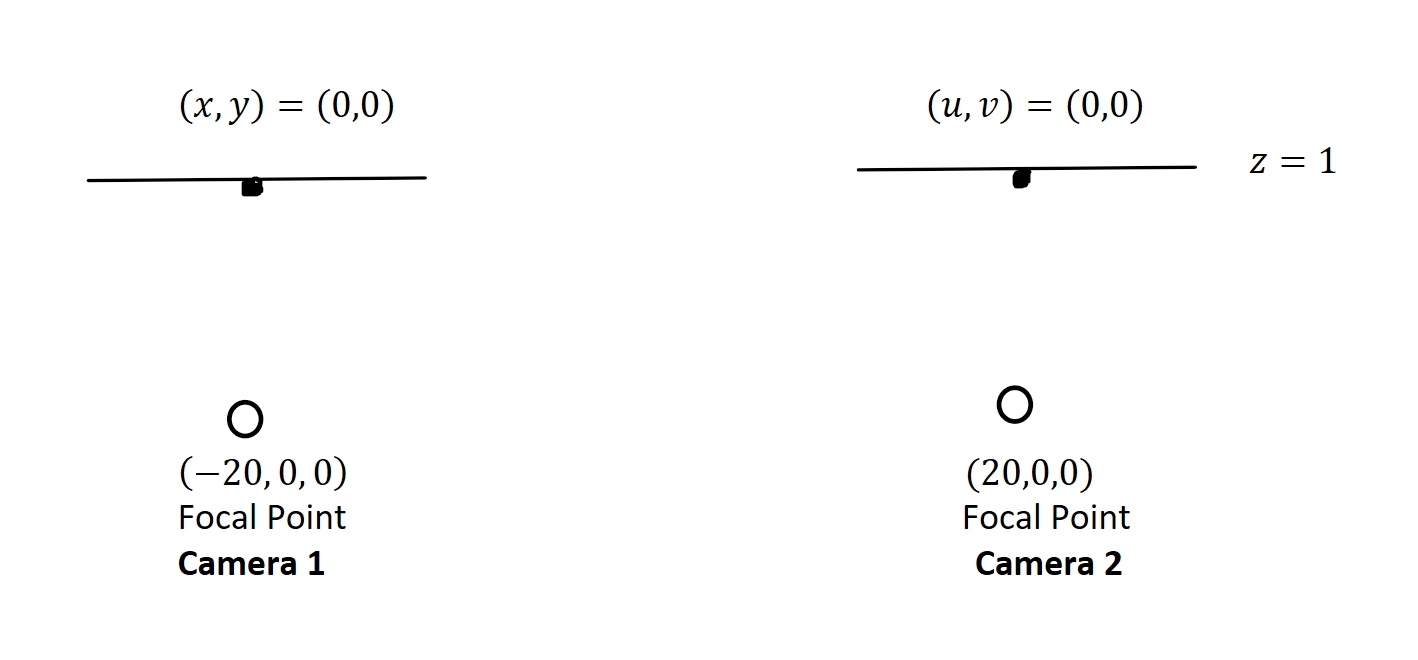
\includegraphics{fig/fig1.png} a) Suppose the points (x, y) = (12,
12) is matched to the point (u, v) = (1, 12). What is the 3D location of
this point?

\begin{enumerate}
\def\labelenumi{\alph{enumi})}
\setcounter{enumi}{1}
\tightlist
\item
  Consider points that lie on the line x + z = 0, y = 0. Use the same
  stereo set up as before. Write an analytic expression giving the
  disparity of a point on this line after it projects onto the two
  images, as a function of its position in the right image. So your
  expression should only involve the variables u and d (for disparity).
  Your expression only needs to be valid for points on the line that are
  in front of the cameras, i.e.~with z \textgreater{} 1.
\end{enumerate}

    \hypertarget{problem-2-epipolar-rectification-4-pts}{%
\subsection{Problem 2: Epipolar Rectification {[}4
pts{]}}\label{problem-2-epipolar-rectification-4-pts}}

In stereo vision, image rectification is a common preprocessing step to
simplify the problem of finding matching points between images. The goal
is to warp image views such that the epipolar lines are horizontal scan
lines of the input images. Suppose that we have captured two images
\(I_A\) and \(I_B\) from identical calibrated cameras separated by a
rigid transformation

\(_{A}^{B}\textrm{T}= \begin{bmatrix} R & t \\ 0^T & 1 \end{bmatrix}\)

Without loss of generality assume that camera A's optical center is
positioned at the origin and that its optical axis is in the direction
of the z-axis.

From the lecture, a rectifying transform for each image should map the
epipole to a point infinitely far away in the horizontal direction \$
H\_\{A\}e\_\{A\} = H\_\{B\}e\_\{B\} = {[}1, 0, 0{]}\^{}T\$. Consider the
following special cases:

\begin{enumerate}
\def\labelenumi{\alph{enumi})}
\item
  Pure horizontal translation \(t = [t_x, 0, 0]^T\), R = I
\item
  Pure translation orthogonal to the optical axis
  \(t = [t_x, t_y, 0]^T\), R = I
\item
  Pure translation along the optical axis \(t = [0, 0, t_z]^T\), R = I
\item
  Pure rotation \(t = [0, 0, 0]^T\), R is an arbitrary rotation matrix
\end{enumerate}

For each of these cases, determine whether or not epipolar rectification
is possible. Include the following information for each case * The
epipoles \(e_A\) and \(e_B\) * The equation of the epipolar line \(l_B\)
in \(I_B\) corresponding to the point \([x_A, y_A, 1]^T\) in \(I_A\) (if
one exists) * A plausible solution to the rectifying transforms \(H_A\)
and \(H_B\) (if one exists) that attempts to minimize distortion (is as
close as possible to a 2D rigid transformation). Note that the above 4
cases are special cases; a simple solution should become apparent by
looking at the epipolar lines.

One or more of the above rigid transformations may be a degenerate case
where rectification is not possible or epipolar geometry does not apply.
If so, explain why.

    \hypertarget{problem-3-filtering-3-pts}{%
\subsection{Problem 3: Filtering {[}3
pts{]}}\label{problem-3-filtering-3-pts}}

\begin{enumerate}
\def\labelenumi{\alph{enumi})}
\item
  Consider smoothing an image with a 3x3 box filter and then computing
  the derivative in the x direction. What is a single convolution kernel
  that will implement this operation?
\item
  Give an example of a separable filter and compare the number of
  arithmetic operations it takes to convolve using that filter on an
  \(n \times n\) image before and after separation.
\end{enumerate}

    \hypertarget{problem-4-sparse-stereo-matching-22-pts}{%
\subsection{Problem 4: Sparse Stereo Matching {[}22
pts{]}}\label{problem-4-sparse-stereo-matching-22-pts}}

    In this problem we will play around with sparse stereo matching methods.
You will work on two image pairs, a warrior figure and a figure from the
Matrix movies. These files both contain two images, two camera matrices,
and set sets of corresponding points (extracted by manually clicking the
images). For illustration, I have run my code on a third image pair
(dino1.png, dino2.png). This data is also provided for you to debug your
code, but you should only report results on warrior and matrix. In other
words, where I include one (or a pair) of images in the assignment
below, you will provide the same thing but for BOTH matrix and warrior.
Note that the matrix image pair is harder, in the sense that the
matching algorithms we are implementing will not work quite as well. You
should expect good results, however, on warrior.

    \hypertarget{corner-detection-5-pts}{%
\subsubsection{4.1 Corner Detection {[}5
pts{]}}\label{corner-detection-5-pts}}

The first thing we need to do is to build a corner detector. This should
be done according to
http://cseweb.ucsd.edu/classes/fa18/cse252A-a/lec11.pdf. You should fill
in the function corner\_detect below, and take as input
corner\_detect(image, nCorners, smoothSTD, windowSize) where smoothSTD
is the standard deviation of the smoothing kernel and windowSize is the
window size for corner detector and non maximum suppression. In the
lecture the corner detector was implemented using a hard threshold. Do
not do that but instead return the nCorners strongest corners after
non-maximum suppression. This way you can control exactly how many
corners are returned. Run your code on all four images (with nCorners =
20) and show outputs as in Figure 2. You may find
scipy.ndimage.filters.gaussian\_filter easy to use for smoothing. In
this problem, try different parameters and then comment on results. 1.
windowSize = 3, 5, 9, 17 2. smoothSTD = 0.5, 1, 2, 4
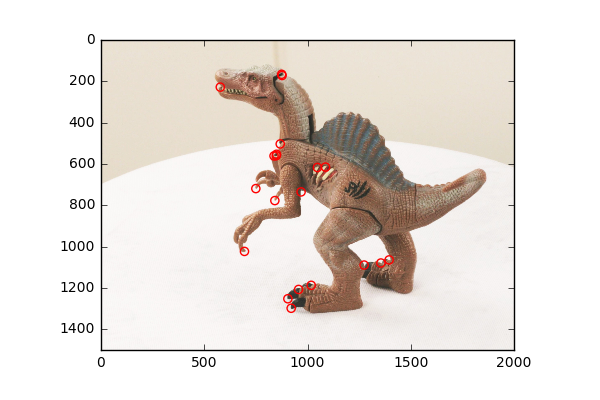
\includegraphics{fig/dinoCorner1.png}
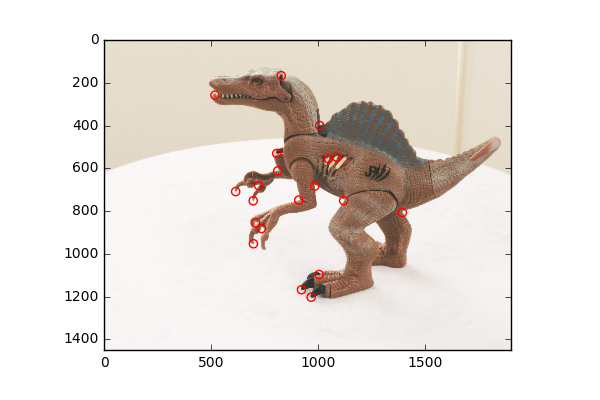
\includegraphics{fig/dinoCorner2.png}

    \begin{Verbatim}[commandchars=\\\{\}]
{\color{incolor}In [{\color{incolor}156}]:} \PY{k+kn}{import} \PY{n+nn}{numpy} \PY{k}{as} \PY{n+nn}{np}
          \PY{k+kn}{from} \PY{n+nn}{scipy}\PY{n+nn}{.}\PY{n+nn}{misc} \PY{k}{import} \PY{n}{imread}
          \PY{k+kn}{import} \PY{n+nn}{matplotlib}\PY{n+nn}{.}\PY{n+nn}{pyplot} \PY{k}{as} \PY{n+nn}{plt}
          \PY{k+kn}{from} \PY{n+nn}{scipy}\PY{n+nn}{.}\PY{n+nn}{ndimage}\PY{n+nn}{.}\PY{n+nn}{filters} \PY{k}{import} \PY{n}{gaussian\PYZus{}filter}
          \PY{k+kn}{import} \PY{n+nn}{cv2}
\end{Verbatim}


    \begin{Verbatim}[commandchars=\\\{\}]
{\color{incolor}In [{\color{incolor}157}]:} \PY{k}{def} \PY{n+nf}{rgb2gray}\PY{p}{(}\PY{n}{rgb}\PY{p}{)}\PY{p}{:}
              \PY{l+s+sd}{\PYZdq{}\PYZdq{}\PYZdq{} Convert rgb image to grayscale.}
          \PY{l+s+sd}{    \PYZdq{}\PYZdq{}\PYZdq{}}
              \PY{k}{return} \PY{n}{np}\PY{o}{.}\PY{n}{dot}\PY{p}{(}\PY{n}{rgb}\PY{p}{[}\PY{o}{.}\PY{o}{.}\PY{o}{.}\PY{p}{,}\PY{p}{:}\PY{l+m+mi}{3}\PY{p}{]}\PY{p}{,} \PY{p}{[}\PY{l+m+mf}{0.299}\PY{p}{,} \PY{l+m+mf}{0.587}\PY{p}{,} \PY{l+m+mf}{0.114}\PY{p}{]}\PY{p}{)}
\end{Verbatim}


    \begin{Verbatim}[commandchars=\\\{\}]
{\color{incolor}In [{\color{incolor}158}]:} \PY{k}{def} \PY{n+nf}{imconv}\PY{p}{(}\PY{n}{img}\PY{p}{,} \PY{n}{operator}\PY{p}{)}\PY{p}{:}
              \PY{n}{conved\PYZus{}img} \PY{o}{=} \PY{n}{np}\PY{o}{.}\PY{n}{zeros}\PY{p}{(}\PY{n}{img}\PY{o}{.}\PY{n}{shape}\PY{p}{)}  
              \PY{n}{r\PYZus{}center} \PY{o}{=} \PY{n+nb}{int}\PY{p}{(}\PY{p}{(}\PY{n}{operator}\PY{o}{.}\PY{n}{shape}\PY{p}{[}\PY{l+m+mi}{0}\PY{p}{]}\PY{o}{\PYZhy{}}\PY{l+m+mi}{1}\PY{p}{)}\PY{o}{/}\PY{l+m+mi}{2}\PY{p}{)}
              \PY{n}{c\PYZus{}center} \PY{o}{=} \PY{n+nb}{int}\PY{p}{(}\PY{p}{(}\PY{n}{operator}\PY{o}{.}\PY{n}{shape}\PY{p}{[}\PY{l+m+mi}{1}\PY{p}{]}\PY{o}{\PYZhy{}}\PY{l+m+mi}{1}\PY{p}{)}\PY{o}{/}\PY{l+m+mi}{2}\PY{p}{)}
              \PY{n}{num\PYZus{}row}\PY{p}{,} \PY{n}{num\PYZus{}col} \PY{o}{=} \PY{n}{img}\PY{o}{.}\PY{n}{shape}
          
              \PY{k}{for} \PY{n}{i} \PY{o+ow}{in} \PY{n+nb}{range}\PY{p}{(}\PY{n}{r\PYZus{}center}\PY{p}{,} \PY{n}{num\PYZus{}row}\PY{o}{\PYZhy{}}\PY{n}{r\PYZus{}center}\PY{p}{)}\PY{p}{:}
                  \PY{k}{for} \PY{n}{j} \PY{o+ow}{in} \PY{n+nb}{range}\PY{p}{(}\PY{n}{c\PYZus{}center}\PY{p}{,} \PY{n}{num\PYZus{}col}\PY{o}{\PYZhy{}}\PY{n}{c\PYZus{}center}\PY{p}{)}\PY{p}{:}
                      \PY{n}{conved\PYZus{}img}\PY{p}{[}\PY{n}{i}\PY{p}{]}\PY{p}{[}\PY{n}{j}\PY{p}{]} \PY{o}{=} \PY{p}{(}\PY{n}{img}\PY{p}{[}\PY{p}{(}\PY{n}{i}\PY{o}{\PYZhy{}}\PY{n}{r\PYZus{}center}\PY{p}{)}\PY{p}{:}\PY{p}{(}\PY{n}{i}\PY{o}{+}\PY{n}{r\PYZus{}center}\PY{o}{+}\PY{l+m+mi}{1}\PY{p}{)}\PY{p}{,}\PYZbs{}
                                              \PY{p}{(}\PY{n}{j}\PY{o}{\PYZhy{}}\PY{n}{c\PYZus{}center}\PY{p}{)}\PY{p}{:}\PY{p}{(}\PY{n}{j}\PY{o}{+}\PY{n}{c\PYZus{}center}\PY{o}{+}\PY{l+m+mi}{1}\PY{p}{)}\PY{p}{]} \PY{o}{*} \PY{n}{operator}\PY{p}{)}\PY{o}{.}\PY{n}{sum}\PY{p}{(}\PY{p}{)}
              \PY{k}{return} \PY{n}{conved\PYZus{}img} \PY{c+c1}{\PYZsh{}[r\PYZus{}center : (num\PYZus{}row\PYZhy{}r\PYZus{}center), c\PYZus{}center : (num\PYZus{}col\PYZhy{}c\PYZus{}center)]}
          
          
          \PY{k}{def} \PY{n+nf}{corner\PYZus{}detect}\PY{p}{(}\PY{n}{image}\PY{p}{,} \PY{n}{nCorners}\PY{p}{,} \PY{n}{smoothSTD}\PY{p}{,} \PY{n}{windowSize}\PY{p}{)}\PY{p}{:}
              \PY{l+s+sd}{\PYZdq{}\PYZdq{}\PYZdq{}Detect corners on a given image.}
          
          \PY{l+s+sd}{    Args:}
          \PY{l+s+sd}{        image: Given a grayscale image on which to detect corners.}
          \PY{l+s+sd}{        nCorners: Total number of corners to be extracted.}
          \PY{l+s+sd}{        smoothSTD: Standard deviation of the Gaussian smoothing kernel.}
          \PY{l+s+sd}{        windowSize: Window size for corner detector and non maximum suppression.}
          
          \PY{l+s+sd}{    Returns:}
          \PY{l+s+sd}{        Detected corners (in image coordinate) in a numpy array (n*2).}
          
          \PY{l+s+sd}{    \PYZdq{}\PYZdq{}\PYZdq{}}
              
              \PY{l+s+sd}{\PYZdq{}\PYZdq{}\PYZdq{}}
          \PY{l+s+sd}{    Your code here:}
          \PY{l+s+sd}{    \PYZdq{}\PYZdq{}\PYZdq{}}
              \PY{n}{smoothed\PYZus{}img} \PY{o}{=} \PY{n}{gaussian\PYZus{}filter}\PY{p}{(}\PY{n}{image}\PY{p}{,}\PY{n}{sigma}\PY{o}{=}\PY{n}{smoothSTD}\PY{p}{)}
              
              \PY{n}{sum\PYZus{}window} \PY{o}{=} \PY{n}{np}\PY{o}{.}\PY{n}{ones}\PY{p}{(}\PY{p}{(}\PY{n}{windowSize}\PY{p}{,} \PY{n}{windowSize}\PY{p}{)}\PY{p}{)}
              \PY{n}{img\PYZus{}dy}\PY{p}{,} \PY{n}{img\PYZus{}dx} \PY{o}{=} \PY{n}{np}\PY{o}{.}\PY{n}{gradient}\PY{p}{(}\PY{n}{smoothed\PYZus{}img}\PY{p}{)} \PY{c+c1}{\PYZsh{} y is row, x i column}
              
              \PY{n}{img\PYZus{}dxdx} \PY{o}{=} \PY{n}{img\PYZus{}dx} \PY{o}{*} \PY{n}{img\PYZus{}dx}
              \PY{n}{img\PYZus{}dydy} \PY{o}{=} \PY{n}{img\PYZus{}dy} \PY{o}{*} \PY{n}{img\PYZus{}dy}
              \PY{n}{img\PYZus{}dxdy} \PY{o}{=} \PY{n}{img\PYZus{}dx} \PY{o}{*} \PY{n}{img\PYZus{}dy}
              \PY{n}{cov\PYZus{}sum\PYZus{}dxdx} \PY{o}{=} \PY{n}{imconv}\PY{p}{(}\PY{n}{img\PYZus{}dxdx}\PY{p}{,} \PY{n}{sum\PYZus{}window}\PY{p}{)}
              \PY{n}{cov\PYZus{}sum\PYZus{}dxdy} \PY{o}{=} \PY{n}{imconv}\PY{p}{(}\PY{n}{img\PYZus{}dxdy}\PY{p}{,} \PY{n}{sum\PYZus{}window}\PY{p}{)}
              \PY{n}{cov\PYZus{}sum\PYZus{}dydy} \PY{o}{=} \PY{n}{imconv}\PY{p}{(}\PY{n}{img\PYZus{}dydy}\PY{p}{,} \PY{n}{sum\PYZus{}window}\PY{p}{)}
              
              \PY{n}{window\PYZus{}center} \PY{o}{=} \PY{n+nb}{int}\PY{p}{(}\PY{p}{(}\PY{n}{windowSize}\PY{o}{\PYZhy{}}\PY{l+m+mi}{1}\PY{p}{)}\PY{o}{/}\PY{l+m+mi}{2}\PY{p}{)}
              \PY{n}{img\PYZus{}lmbd} \PY{o}{=} \PY{n}{np}\PY{o}{.}\PY{n}{zeros}\PY{p}{(}\PY{n}{image}\PY{o}{.}\PY{n}{shape}\PY{p}{)}
              \PY{k}{for} \PY{n}{i} \PY{o+ow}{in} \PY{n+nb}{range}\PY{p}{(}\PY{n}{image}\PY{o}{.}\PY{n}{shape}\PY{p}{[}\PY{l+m+mi}{0}\PY{p}{]}\PY{p}{)}\PY{p}{:}
                  \PY{k}{for} \PY{n}{j} \PY{o+ow}{in} \PY{n+nb}{range}\PY{p}{(}\PY{n}{image}\PY{o}{.}\PY{n}{shape}\PY{p}{[}\PY{l+m+mi}{1}\PY{p}{]}\PY{p}{)}\PY{p}{:}
                      \PY{n}{covariance} \PY{o}{=} \PY{n}{np}\PY{o}{.}\PY{n}{array}\PY{p}{(}\PY{p}{[}\PY{p}{[}\PY{n}{cov\PYZus{}sum\PYZus{}dxdx}\PY{p}{[}\PY{n}{i}\PY{p}{]}\PY{p}{[}\PY{n}{j}\PY{p}{]}\PY{p}{,} \PY{n}{cov\PYZus{}sum\PYZus{}dxdy}\PY{p}{[}\PY{n}{i}\PY{p}{]}\PY{p}{[}\PY{n}{j}\PY{p}{]}\PY{p}{]}\PY{p}{,}\PYZbs{}
                                             \PY{p}{[}\PY{n}{cov\PYZus{}sum\PYZus{}dxdy}\PY{p}{[}\PY{n}{i}\PY{p}{]}\PY{p}{[}\PY{n}{j}\PY{p}{]}\PY{p}{,} \PY{n}{cov\PYZus{}sum\PYZus{}dydy}\PY{p}{[}\PY{n}{i}\PY{p}{]}\PY{p}{[}\PY{n}{j}\PY{p}{]}\PY{p}{]}\PY{p}{]}\PY{p}{)}
                      \PY{n}{lmbds}\PY{p}{,} \PY{n}{egnvctrs} \PY{o}{=} \PY{n}{np}\PY{o}{.}\PY{n}{linalg}\PY{o}{.}\PY{n}{eig}\PY{p}{(}\PY{n}{covariance}\PY{p}{)}
                      \PY{n}{img\PYZus{}lmbd}\PY{p}{[}\PY{n}{i}\PY{p}{]}\PY{p}{[}\PY{n}{j}\PY{p}{]} \PY{o}{=} \PY{n+nb}{min}\PY{p}{(}\PY{n}{lmbds}\PY{p}{)}
              
              
              \PY{n}{corner\PYZus{}coord\PYZus{}cndts} \PY{o}{=} \PY{p}{[}\PY{p}{]}
              \PY{n}{corner\PYZus{}lmbd\PYZus{}cndts} \PY{o}{=} \PY{p}{[}\PY{p}{]}
              \PY{k}{for} \PY{n}{i} \PY{o+ow}{in} \PY{n+nb}{range}\PY{p}{(}\PY{n}{window\PYZus{}center}\PY{p}{,} \PY{n}{image}\PY{o}{.}\PY{n}{shape}\PY{p}{[}\PY{l+m+mi}{0}\PY{p}{]}\PY{o}{\PYZhy{}}\PY{n}{window\PYZus{}center}\PY{p}{)}\PY{p}{:}
                  \PY{k}{for} \PY{n}{j} \PY{o+ow}{in} \PY{n+nb}{range}\PY{p}{(}\PY{n}{window\PYZus{}center}\PY{p}{,} \PY{n}{image}\PY{o}{.}\PY{n}{shape}\PY{p}{[}\PY{l+m+mi}{1}\PY{p}{]}\PY{o}{\PYZhy{}}\PY{n}{window\PYZus{}center}\PY{p}{)}\PY{p}{:}
                      
                      \PY{n}{patch\PYZus{}lmbd} \PY{o}{=} \PY{n}{img\PYZus{}lmbd}\PY{p}{[}\PY{n}{i}\PY{o}{\PYZhy{}}\PY{n}{window\PYZus{}center}\PY{p}{:} \PY{n}{i}\PY{o}{+}\PY{n}{window\PYZus{}center}\PY{o}{+}\PY{l+m+mi}{1}\PY{p}{,}\PYZbs{}
                                            \PY{n}{j}\PY{o}{\PYZhy{}}\PY{n}{window\PYZus{}center}\PY{p}{:} \PY{n}{j}\PY{o}{+}\PY{n}{window\PYZus{}center}\PY{o}{+}\PY{l+m+mi}{1}\PY{p}{]}
                      
                      \PY{k}{if} \PY{n}{patch\PYZus{}lmbd}\PY{p}{[}\PY{n}{window\PYZus{}center}\PY{p}{]}\PY{p}{[}\PY{n}{window\PYZus{}center}\PY{p}{]} \PY{o}{==} \PY{n}{np}\PY{o}{.}\PY{n}{max}\PY{p}{(}\PY{n}{patch\PYZus{}lmbd}\PY{p}{)}\PY{p}{:}
                          \PY{c+c1}{\PYZsh{} it is local maximum}
                          \PY{n}{corner\PYZus{}coord\PYZus{}cndts}\PY{o}{.}\PY{n}{append}\PY{p}{(}\PY{p}{[}\PY{n}{j}\PY{p}{,} \PY{n}{i}\PY{p}{]}\PY{p}{)} \PY{c+c1}{\PYZsh{} y, x}
                          \PY{n}{corner\PYZus{}lmbd\PYZus{}cndts}\PY{o}{.}\PY{n}{append}\PY{p}{(}\PY{n}{np}\PY{o}{.}\PY{n}{max}\PY{p}{(}\PY{n}{patch\PYZus{}lmbd}\PY{p}{)}\PY{p}{)} 
                          
              
              \PY{n}{corner\PYZus{}lmbd\PYZus{}cndts} \PY{o}{=} \PY{n}{np}\PY{o}{.}\PY{n}{array}\PY{p}{(}\PY{n}{corner\PYZus{}lmbd\PYZus{}cndts}\PY{p}{)}\PY{p}{[}\PY{p}{:}\PY{p}{,} \PY{k+kc}{None}\PY{p}{]}
              \PY{n}{corner\PYZus{}coord\PYZus{}cndts} \PY{o}{=} \PY{n}{np}\PY{o}{.}\PY{n}{array}\PY{p}{(}\PY{n}{corner\PYZus{}coord\PYZus{}cndts}\PY{p}{)}
              
              \PY{n}{unique\PYZus{}corner\PYZus{}lmbds} \PY{o}{=} \PY{n}{np}\PY{o}{.}\PY{n}{sort}\PY{p}{(}\PY{n}{corner\PYZus{}lmbd\PYZus{}cndts}\PY{p}{,} \PY{n}{axis}\PY{o}{=}\PY{l+m+mi}{0}\PY{p}{)}
              \PY{n}{threshold} \PY{o}{=} \PY{n}{unique\PYZus{}corner\PYZus{}lmbds}\PY{p}{[}\PY{o}{\PYZhy{}}\PY{n}{nCorners}\PY{p}{]}
              \PY{n}{idx\PYZus{}row}\PY{p}{,} \PY{n}{idx\PYZus{}col} \PY{o}{=} \PY{n}{np}\PY{o}{.}\PY{n}{where}\PY{p}{(}\PY{n}{corner\PYZus{}lmbd\PYZus{}cndts} \PY{o}{\PYZgt{}} \PY{n}{threshold}\PY{p}{)}
              \PY{n}{corners} \PY{o}{=} \PY{n}{corner\PYZus{}coord\PYZus{}cndts}\PY{p}{[}\PY{n}{idx\PYZus{}row}\PY{p}{]}
              \PY{k}{return} \PY{n}{corners} \PY{c+c1}{\PYZsh{}corners N *3}
          
          
          \PY{k}{def} \PY{n+nf}{show\PYZus{}corners\PYZus{}result}\PY{p}{(}\PY{n}{imgs}\PY{p}{,} \PY{n}{corners}\PY{p}{)}\PY{p}{:}
              \PY{n}{fig} \PY{o}{=} \PY{n}{plt}\PY{o}{.}\PY{n}{figure}\PY{p}{(}\PY{n}{figsize}\PY{o}{=}\PY{p}{(}\PY{l+m+mi}{8}\PY{p}{,} \PY{l+m+mi}{8}\PY{p}{)}\PY{p}{)}
              \PY{n}{ax1} \PY{o}{=} \PY{n}{fig}\PY{o}{.}\PY{n}{add\PYZus{}subplot}\PY{p}{(}\PY{l+m+mi}{221}\PY{p}{)}
              \PY{n}{ax1}\PY{o}{.}\PY{n}{imshow}\PY{p}{(}\PY{n}{imgs}\PY{p}{[}\PY{l+m+mi}{0}\PY{p}{]}\PY{p}{,} \PY{n}{cmap}\PY{o}{=}\PY{l+s+s1}{\PYZsq{}}\PY{l+s+s1}{gray}\PY{l+s+s1}{\PYZsq{}}\PY{p}{)}
              \PY{n}{ax1}\PY{o}{.}\PY{n}{scatter}\PY{p}{(}\PY{n}{corners}\PY{p}{[}\PY{l+m+mi}{0}\PY{p}{]}\PY{p}{[}\PY{p}{:}\PY{p}{,} \PY{l+m+mi}{0}\PY{p}{]}\PY{p}{,} \PY{n}{corners}\PY{p}{[}\PY{l+m+mi}{0}\PY{p}{]}\PY{p}{[}\PY{p}{:}\PY{p}{,} \PY{l+m+mi}{1}\PY{p}{]}\PY{p}{,} \PY{n}{s}\PY{o}{=}\PY{l+m+mi}{35}\PY{p}{,} \PY{n}{edgecolors}\PY{o}{=}\PY{l+s+s1}{\PYZsq{}}\PY{l+s+s1}{r}\PY{l+s+s1}{\PYZsq{}}\PY{p}{,} \PY{n}{facecolors}\PY{o}{=}\PY{l+s+s1}{\PYZsq{}}\PY{l+s+s1}{none}\PY{l+s+s1}{\PYZsq{}}\PY{p}{)}
          
              \PY{n}{ax2} \PY{o}{=} \PY{n}{fig}\PY{o}{.}\PY{n}{add\PYZus{}subplot}\PY{p}{(}\PY{l+m+mi}{222}\PY{p}{)}
              \PY{n}{ax2}\PY{o}{.}\PY{n}{imshow}\PY{p}{(}\PY{n}{imgs}\PY{p}{[}\PY{l+m+mi}{1}\PY{p}{]}\PY{p}{,} \PY{n}{cmap}\PY{o}{=}\PY{l+s+s1}{\PYZsq{}}\PY{l+s+s1}{gray}\PY{l+s+s1}{\PYZsq{}}\PY{p}{)}
              \PY{n}{ax2}\PY{o}{.}\PY{n}{scatter}\PY{p}{(}\PY{n}{corners}\PY{p}{[}\PY{l+m+mi}{1}\PY{p}{]}\PY{p}{[}\PY{p}{:}\PY{p}{,} \PY{l+m+mi}{0}\PY{p}{]}\PY{p}{,} \PY{n}{corners}\PY{p}{[}\PY{l+m+mi}{1}\PY{p}{]}\PY{p}{[}\PY{p}{:}\PY{p}{,} \PY{l+m+mi}{1}\PY{p}{]}\PY{p}{,} \PY{n}{s}\PY{o}{=}\PY{l+m+mi}{35}\PY{p}{,} \PY{n}{edgecolors}\PY{o}{=}\PY{l+s+s1}{\PYZsq{}}\PY{l+s+s1}{r}\PY{l+s+s1}{\PYZsq{}}\PY{p}{,} \PY{n}{facecolors}\PY{o}{=}\PY{l+s+s1}{\PYZsq{}}\PY{l+s+s1}{none}\PY{l+s+s1}{\PYZsq{}}\PY{p}{)}
              \PY{n}{plt}\PY{o}{.}\PY{n}{show}\PY{p}{(}\PY{p}{)}
\end{Verbatim}


    \begin{Verbatim}[commandchars=\\\{\}]
{\color{incolor}In [{\color{incolor}159}]:} \PY{c+c1}{\PYZsh{} detect corners on warrior and matrix sets}
          \PY{c+c1}{\PYZsh{} adjust your corner detection parameters here}
          \PY{n}{nCorners} \PY{o}{=} \PY{l+m+mi}{20}
          \PY{n}{windowSize} \PY{o}{=} \PY{l+m+mi}{3}
          \PY{n}{smoothSTD} \PY{o}{=} \PY{l+m+mf}{0.5}
          
          \PY{c+c1}{\PYZsh{} read images and detect corners on images}
          \PY{n}{imgs\PYZus{}mat} \PY{o}{=} \PY{p}{[}\PY{p}{]}
          \PY{n}{crns\PYZus{}mat} \PY{o}{=} \PY{p}{[}\PY{p}{]}
          \PY{n}{imgs\PYZus{}war} \PY{o}{=} \PY{p}{[}\PY{p}{]}
          \PY{n}{crns\PYZus{}war} \PY{o}{=} \PY{p}{[}\PY{p}{]}
          \PY{k}{for} \PY{n}{i} \PY{o+ow}{in} \PY{n+nb}{range}\PY{p}{(}\PY{l+m+mi}{2}\PY{p}{)}\PY{p}{:}
              \PY{n}{img\PYZus{}mat} \PY{o}{=} \PY{n}{imread}\PY{p}{(}\PY{l+s+s1}{\PYZsq{}}\PY{l+s+s1}{p4/matrix/matrix}\PY{l+s+s1}{\PYZsq{}} \PY{o}{+} \PY{n+nb}{str}\PY{p}{(}\PY{n}{i}\PY{p}{)} \PY{o}{+} \PY{l+s+s1}{\PYZsq{}}\PY{l+s+s1}{.png}\PY{l+s+s1}{\PYZsq{}}\PY{p}{)}
              \PY{n}{imgs\PYZus{}mat}\PY{o}{.}\PY{n}{append}\PY{p}{(}\PY{n}{rgb2gray}\PY{p}{(}\PY{n}{img\PYZus{}mat}\PY{p}{)}\PY{p}{)}
              \PY{c+c1}{\PYZsh{} downsize your image in case corner\PYZus{}detect runs slow in test}
              \PY{c+c1}{\PYZsh{} imgs\PYZus{}mat.append(rgb2gray(img\PYZus{}mat)[::2, ::2])}
              \PY{n}{crns\PYZus{}mat}\PY{o}{.}\PY{n}{append}\PY{p}{(}\PY{n}{corner\PYZus{}detect}\PY{p}{(}\PY{n}{imgs\PYZus{}mat}\PY{p}{[}\PY{n}{i}\PY{p}{]}\PY{p}{,} \PY{n}{nCorners}\PY{p}{,} \PY{n}{smoothSTD}\PY{p}{,} \PY{n}{windowSize}\PY{p}{)}\PY{p}{)}
              
              \PY{n}{img\PYZus{}war} \PY{o}{=} \PY{n}{imread}\PY{p}{(}\PY{l+s+s1}{\PYZsq{}}\PY{l+s+s1}{p4/warrior/warrior}\PY{l+s+s1}{\PYZsq{}} \PY{o}{+} \PY{n+nb}{str}\PY{p}{(}\PY{n}{i}\PY{p}{)} \PY{o}{+} \PY{l+s+s1}{\PYZsq{}}\PY{l+s+s1}{.png}\PY{l+s+s1}{\PYZsq{}}\PY{p}{)}
              \PY{n}{imgs\PYZus{}war}\PY{o}{.}\PY{n}{append}\PY{p}{(}\PY{n}{rgb2gray}\PY{p}{(}\PY{n}{img\PYZus{}war}\PY{p}{)}\PY{p}{)}
              \PY{c+c1}{\PYZsh{} downsize your image in case corner\PYZus{}detect runs slow in test}
              \PY{c+c1}{\PYZsh{} imgs\PYZus{}war.append(rgb2gray(img\PYZus{}war)[::2, ::2])}
              \PY{n}{crns\PYZus{}war}\PY{o}{.}\PY{n}{append}\PY{p}{(}\PY{n}{corner\PYZus{}detect}\PY{p}{(}\PY{n}{imgs\PYZus{}war}\PY{p}{[}\PY{n}{i}\PY{p}{]}\PY{p}{,} \PY{n}{nCorners}\PY{p}{,} \PY{n}{smoothSTD}\PY{p}{,} \PY{n}{windowSize}\PY{p}{)}\PY{p}{)}
              
          \PY{n}{show\PYZus{}corners\PYZus{}result}\PY{p}{(}\PY{n}{imgs\PYZus{}mat}\PY{p}{,} \PY{n}{crns\PYZus{}mat}\PY{p}{)}
          \PY{n}{show\PYZus{}corners\PYZus{}result}\PY{p}{(}\PY{n}{imgs\PYZus{}war}\PY{p}{,} \PY{n}{crns\PYZus{}war}\PY{p}{)}
\end{Verbatim}


    \begin{Verbatim}[commandchars=\\\{\}]
/usr/local/lib/python3.7/site-packages/ipykernel\_launcher.py:13: DeprecationWarning: `imread` is deprecated!
`imread` is deprecated in SciPy 1.0.0, and will be removed in 1.2.0.
Use ``imageio.imread`` instead.
  del sys.path[0]
/usr/local/lib/python3.7/site-packages/ipykernel\_launcher.py:19: DeprecationWarning: `imread` is deprecated!
`imread` is deprecated in SciPy 1.0.0, and will be removed in 1.2.0.
Use ``imageio.imread`` instead.

    \end{Verbatim}

    \begin{center}
    \adjustimage{max size={0.9\linewidth}{0.9\paperheight}}{output_10_1.png}
    \end{center}
    { \hspace*{\fill} \\}
    
    \begin{center}
    \adjustimage{max size={0.9\linewidth}{0.9\paperheight}}{output_10_2.png}
    \end{center}
    { \hspace*{\fill} \\}
    
    \begin{Verbatim}[commandchars=\\\{\}]
{\color{incolor}In [{\color{incolor}160}]:} \PY{n}{nCorners} \PY{o}{=} \PY{l+m+mi}{20}
          \PY{k}{for} \PY{n}{windowSize} \PY{o+ow}{in} \PY{p}{[}\PY{l+m+mi}{3}\PY{p}{,} \PY{l+m+mi}{5}\PY{p}{,} \PY{l+m+mi}{9}\PY{p}{,} \PY{l+m+mi}{17}\PY{p}{]}\PY{p}{:}
              \PY{k}{for} \PY{n}{smoothSTD} \PY{o+ow}{in} \PY{p}{[}\PY{l+m+mf}{0.5}\PY{p}{,} \PY{l+m+mi}{1}\PY{p}{,} \PY{l+m+mi}{2}\PY{p}{,} \PY{l+m+mi}{4}\PY{p}{]}\PY{p}{:}
                  \PY{n+nb}{print}\PY{p}{(}\PY{l+s+s1}{\PYZsq{}}\PY{l+s+s1}{windowSize is }\PY{l+s+si}{\PYZob{}0\PYZcb{}}\PY{l+s+s1}{, and smoothSTD is }\PY{l+s+si}{\PYZob{}1\PYZcb{}}\PY{l+s+s1}{\PYZsq{}}\PY{o}{.}\PY{n}{format}\PY{p}{(}\PY{n}{windowSize}\PY{p}{,} \PY{n}{smoothSTD}\PY{p}{)}\PY{p}{)}
                  \PY{c+c1}{\PYZsh{} read images and detect corners on images}
                  \PY{n}{imgs\PYZus{}mat} \PY{o}{=} \PY{p}{[}\PY{p}{]}
                  \PY{n}{crns\PYZus{}mat} \PY{o}{=} \PY{p}{[}\PY{p}{]}
                  \PY{n}{imgs\PYZus{}war} \PY{o}{=} \PY{p}{[}\PY{p}{]}
                  \PY{n}{crns\PYZus{}war} \PY{o}{=} \PY{p}{[}\PY{p}{]}
                  \PY{k}{for} \PY{n}{i} \PY{o+ow}{in} \PY{n+nb}{range}\PY{p}{(}\PY{l+m+mi}{2}\PY{p}{)}\PY{p}{:}
                      \PY{n}{img\PYZus{}mat} \PY{o}{=} \PY{n}{imread}\PY{p}{(}\PY{l+s+s1}{\PYZsq{}}\PY{l+s+s1}{p4/matrix/matrix}\PY{l+s+s1}{\PYZsq{}} \PY{o}{+} \PY{n+nb}{str}\PY{p}{(}\PY{n}{i}\PY{p}{)} \PY{o}{+} \PY{l+s+s1}{\PYZsq{}}\PY{l+s+s1}{.png}\PY{l+s+s1}{\PYZsq{}}\PY{p}{)}
                      \PY{n}{imgs\PYZus{}mat}\PY{o}{.}\PY{n}{append}\PY{p}{(}\PY{n}{rgb2gray}\PY{p}{(}\PY{n}{img\PYZus{}mat}\PY{p}{)}\PY{p}{)}
                      \PY{c+c1}{\PYZsh{} downsize your image in case corner\PYZus{}detect runs slow in test}
                      \PY{c+c1}{\PYZsh{} imgs\PYZus{}mat.append(rgb2gray(img\PYZus{}mat)[::2, ::2])}
                      \PY{n}{crns\PYZus{}mat}\PY{o}{.}\PY{n}{append}\PY{p}{(}\PY{n}{corner\PYZus{}detect}\PY{p}{(}\PY{n}{imgs\PYZus{}mat}\PY{p}{[}\PY{n}{i}\PY{p}{]}\PY{p}{,} \PY{n}{nCorners}\PY{p}{,} \PY{n}{smoothSTD}\PY{p}{,} \PY{n}{windowSize}\PY{p}{)}\PY{p}{)}
          
                      \PY{n}{img\PYZus{}war} \PY{o}{=} \PY{n}{imread}\PY{p}{(}\PY{l+s+s1}{\PYZsq{}}\PY{l+s+s1}{p4/warrior/warrior}\PY{l+s+s1}{\PYZsq{}} \PY{o}{+} \PY{n+nb}{str}\PY{p}{(}\PY{n}{i}\PY{p}{)} \PY{o}{+} \PY{l+s+s1}{\PYZsq{}}\PY{l+s+s1}{.png}\PY{l+s+s1}{\PYZsq{}}\PY{p}{)}
                      \PY{n}{imgs\PYZus{}war}\PY{o}{.}\PY{n}{append}\PY{p}{(}\PY{n}{rgb2gray}\PY{p}{(}\PY{n}{img\PYZus{}war}\PY{p}{)}\PY{p}{)}
                      \PY{c+c1}{\PYZsh{} downsize your image in case corner\PYZus{}detect runs slow in test}
                      \PY{c+c1}{\PYZsh{} imgs\PYZus{}war.append(rgb2gray(img\PYZus{}war)[::2, ::2])}
                      \PY{n}{crns\PYZus{}war}\PY{o}{.}\PY{n}{append}\PY{p}{(}\PY{n}{corner\PYZus{}detect}\PY{p}{(}\PY{n}{imgs\PYZus{}war}\PY{p}{[}\PY{n}{i}\PY{p}{]}\PY{p}{,} \PY{n}{nCorners}\PY{p}{,} \PY{n}{smoothSTD}\PY{p}{,} \PY{n}{windowSize}\PY{p}{)}\PY{p}{)}
          
                  \PY{n}{show\PYZus{}corners\PYZus{}result}\PY{p}{(}\PY{n}{imgs\PYZus{}mat}\PY{p}{,} \PY{n}{crns\PYZus{}mat}\PY{p}{)}
                  \PY{n}{show\PYZus{}corners\PYZus{}result}\PY{p}{(}\PY{n}{imgs\PYZus{}war}\PY{p}{,} \PY{n}{crns\PYZus{}war}\PY{p}{)}
                  \PY{n+nb}{print}\PY{p}{(}\PY{l+s+s1}{\PYZsq{}}\PY{l+s+se}{\PYZbs{}n}\PY{l+s+s1}{\PYZsq{}}\PY{p}{)}
\end{Verbatim}


    \begin{Verbatim}[commandchars=\\\{\}]
windowSize is 3, and smoothSTD is 0.5

    \end{Verbatim}

    \begin{Verbatim}[commandchars=\\\{\}]
/usr/local/lib/python3.7/site-packages/ipykernel\_launcher.py:11: DeprecationWarning: `imread` is deprecated!
`imread` is deprecated in SciPy 1.0.0, and will be removed in 1.2.0.
Use ``imageio.imread`` instead.
  \# This is added back by InteractiveShellApp.init\_path()
/usr/local/lib/python3.7/site-packages/ipykernel\_launcher.py:17: DeprecationWarning: `imread` is deprecated!
`imread` is deprecated in SciPy 1.0.0, and will be removed in 1.2.0.
Use ``imageio.imread`` instead.

    \end{Verbatim}

    \begin{center}
    \adjustimage{max size={0.9\linewidth}{0.9\paperheight}}{output_11_2.png}
    \end{center}
    { \hspace*{\fill} \\}
    
    \begin{center}
    \adjustimage{max size={0.9\linewidth}{0.9\paperheight}}{output_11_3.png}
    \end{center}
    { \hspace*{\fill} \\}
    
    \begin{Verbatim}[commandchars=\\\{\}]


windowSize is 3, and smoothSTD is 1

    \end{Verbatim}

    \begin{center}
    \adjustimage{max size={0.9\linewidth}{0.9\paperheight}}{output_11_5.png}
    \end{center}
    { \hspace*{\fill} \\}
    
    \begin{center}
    \adjustimage{max size={0.9\linewidth}{0.9\paperheight}}{output_11_6.png}
    \end{center}
    { \hspace*{\fill} \\}
    
    \begin{Verbatim}[commandchars=\\\{\}]


windowSize is 3, and smoothSTD is 2

    \end{Verbatim}

    \begin{center}
    \adjustimage{max size={0.9\linewidth}{0.9\paperheight}}{output_11_8.png}
    \end{center}
    { \hspace*{\fill} \\}
    
    \begin{center}
    \adjustimage{max size={0.9\linewidth}{0.9\paperheight}}{output_11_9.png}
    \end{center}
    { \hspace*{\fill} \\}
    
    \begin{Verbatim}[commandchars=\\\{\}]


windowSize is 3, and smoothSTD is 4

    \end{Verbatim}

    \begin{center}
    \adjustimage{max size={0.9\linewidth}{0.9\paperheight}}{output_11_11.png}
    \end{center}
    { \hspace*{\fill} \\}
    
    \begin{center}
    \adjustimage{max size={0.9\linewidth}{0.9\paperheight}}{output_11_12.png}
    \end{center}
    { \hspace*{\fill} \\}
    
    \begin{Verbatim}[commandchars=\\\{\}]


windowSize is 5, and smoothSTD is 0.5

    \end{Verbatim}

    \begin{center}
    \adjustimage{max size={0.9\linewidth}{0.9\paperheight}}{output_11_14.png}
    \end{center}
    { \hspace*{\fill} \\}
    
    \begin{center}
    \adjustimage{max size={0.9\linewidth}{0.9\paperheight}}{output_11_15.png}
    \end{center}
    { \hspace*{\fill} \\}
    
    \begin{Verbatim}[commandchars=\\\{\}]


windowSize is 5, and smoothSTD is 1

    \end{Verbatim}

    \begin{center}
    \adjustimage{max size={0.9\linewidth}{0.9\paperheight}}{output_11_17.png}
    \end{center}
    { \hspace*{\fill} \\}
    
    \begin{center}
    \adjustimage{max size={0.9\linewidth}{0.9\paperheight}}{output_11_18.png}
    \end{center}
    { \hspace*{\fill} \\}
    
    \begin{Verbatim}[commandchars=\\\{\}]


windowSize is 5, and smoothSTD is 2

    \end{Verbatim}

    \begin{center}
    \adjustimage{max size={0.9\linewidth}{0.9\paperheight}}{output_11_20.png}
    \end{center}
    { \hspace*{\fill} \\}
    
    \begin{center}
    \adjustimage{max size={0.9\linewidth}{0.9\paperheight}}{output_11_21.png}
    \end{center}
    { \hspace*{\fill} \\}
    
    \begin{Verbatim}[commandchars=\\\{\}]


windowSize is 5, and smoothSTD is 4

    \end{Verbatim}

    \begin{center}
    \adjustimage{max size={0.9\linewidth}{0.9\paperheight}}{output_11_23.png}
    \end{center}
    { \hspace*{\fill} \\}
    
    \begin{center}
    \adjustimage{max size={0.9\linewidth}{0.9\paperheight}}{output_11_24.png}
    \end{center}
    { \hspace*{\fill} \\}
    
    \begin{Verbatim}[commandchars=\\\{\}]


windowSize is 9, and smoothSTD is 0.5

    \end{Verbatim}

    \begin{center}
    \adjustimage{max size={0.9\linewidth}{0.9\paperheight}}{output_11_26.png}
    \end{center}
    { \hspace*{\fill} \\}
    
    \begin{center}
    \adjustimage{max size={0.9\linewidth}{0.9\paperheight}}{output_11_27.png}
    \end{center}
    { \hspace*{\fill} \\}
    
    \begin{Verbatim}[commandchars=\\\{\}]


windowSize is 9, and smoothSTD is 1

    \end{Verbatim}

    \begin{center}
    \adjustimage{max size={0.9\linewidth}{0.9\paperheight}}{output_11_29.png}
    \end{center}
    { \hspace*{\fill} \\}
    
    \begin{center}
    \adjustimage{max size={0.9\linewidth}{0.9\paperheight}}{output_11_30.png}
    \end{center}
    { \hspace*{\fill} \\}
    
    \begin{Verbatim}[commandchars=\\\{\}]


windowSize is 9, and smoothSTD is 2

    \end{Verbatim}

    \begin{center}
    \adjustimage{max size={0.9\linewidth}{0.9\paperheight}}{output_11_32.png}
    \end{center}
    { \hspace*{\fill} \\}
    
    \begin{center}
    \adjustimage{max size={0.9\linewidth}{0.9\paperheight}}{output_11_33.png}
    \end{center}
    { \hspace*{\fill} \\}
    
    \begin{Verbatim}[commandchars=\\\{\}]


windowSize is 9, and smoothSTD is 4

    \end{Verbatim}

    \begin{center}
    \adjustimage{max size={0.9\linewidth}{0.9\paperheight}}{output_11_35.png}
    \end{center}
    { \hspace*{\fill} \\}
    
    \begin{center}
    \adjustimage{max size={0.9\linewidth}{0.9\paperheight}}{output_11_36.png}
    \end{center}
    { \hspace*{\fill} \\}
    
    \begin{Verbatim}[commandchars=\\\{\}]


windowSize is 17, and smoothSTD is 0.5

    \end{Verbatim}

    \begin{center}
    \adjustimage{max size={0.9\linewidth}{0.9\paperheight}}{output_11_38.png}
    \end{center}
    { \hspace*{\fill} \\}
    
    \begin{center}
    \adjustimage{max size={0.9\linewidth}{0.9\paperheight}}{output_11_39.png}
    \end{center}
    { \hspace*{\fill} \\}
    
    \begin{Verbatim}[commandchars=\\\{\}]


windowSize is 17, and smoothSTD is 1

    \end{Verbatim}

    \begin{center}
    \adjustimage{max size={0.9\linewidth}{0.9\paperheight}}{output_11_41.png}
    \end{center}
    { \hspace*{\fill} \\}
    
    \begin{center}
    \adjustimage{max size={0.9\linewidth}{0.9\paperheight}}{output_11_42.png}
    \end{center}
    { \hspace*{\fill} \\}
    
    \begin{Verbatim}[commandchars=\\\{\}]


windowSize is 17, and smoothSTD is 2

    \end{Verbatim}

    \begin{center}
    \adjustimage{max size={0.9\linewidth}{0.9\paperheight}}{output_11_44.png}
    \end{center}
    { \hspace*{\fill} \\}
    
    \begin{center}
    \adjustimage{max size={0.9\linewidth}{0.9\paperheight}}{output_11_45.png}
    \end{center}
    { \hspace*{\fill} \\}
    
    \begin{Verbatim}[commandchars=\\\{\}]


windowSize is 17, and smoothSTD is 4

    \end{Verbatim}

    \begin{center}
    \adjustimage{max size={0.9\linewidth}{0.9\paperheight}}{output_11_47.png}
    \end{center}
    { \hspace*{\fill} \\}
    
    \begin{center}
    \adjustimage{max size={0.9\linewidth}{0.9\paperheight}}{output_11_48.png}
    \end{center}
    { \hspace*{\fill} \\}
    
    \begin{Verbatim}[commandchars=\\\{\}]



    \end{Verbatim}

    In general corner detection works well on large smoothSTD, since with
large smoothSTD, some detail being averaged, the detection algorithm can
focus on more abstract corner features. Also, with relative large window
size, the detection variance can be decreased, which can make detection
more accurate.

    \hypertarget{ncc-normalized-cross-correlation-matching-2-pts}{%
\subsubsection{NCC (Normalized Cross-Correlation) Matching {[}2
pts{]}}\label{ncc-normalized-cross-correlation-matching-2-pts}}

Write a function ncc\_match that implements the NCC matching algorithm
for two input windows. NCC =
\(\sum_{i,j}\tilde{W_1} (i,j)\cdot \tilde{W_2} (i,j)\) where
\(\tilde{W} = \frac{W - \overline{W}}{\sqrt{\sum_{k,l}(W(k,l) - \overline{W})^2}}\)
is a mean-shifted and normalized version of the window and
\(\overline{W}\) is the mean pixel value in the window W.

    \begin{Verbatim}[commandchars=\\\{\}]
{\color{incolor}In [{\color{incolor}7}]:} \PY{k}{def} \PY{n+nf}{ncc\PYZus{}match}\PY{p}{(}\PY{n}{img1}\PY{p}{,} \PY{n}{img2}\PY{p}{,} \PY{n}{c1}\PY{p}{,} \PY{n}{c2}\PY{p}{,} \PY{n}{R}\PY{p}{)}\PY{p}{:}
            \PY{l+s+sd}{\PYZdq{}\PYZdq{}\PYZdq{}Compute NCC given two windows.}
        
        \PY{l+s+sd}{    Args:}
        \PY{l+s+sd}{        img1: Image 1.}
        \PY{l+s+sd}{        img2: Image 2.}
        \PY{l+s+sd}{        c1: Center (in image coordinate) of the window in image 1.}
        \PY{l+s+sd}{        c2: Center (in image coordinate) of the window in image 2.}
        \PY{l+s+sd}{        R: R is the radius of the patch, 2 * R + 1 is the window size}
        
        \PY{l+s+sd}{    Returns:}
        \PY{l+s+sd}{        NCC matching score for two input windows.}
        
        \PY{l+s+sd}{    \PYZdq{}\PYZdq{}\PYZdq{}}
            
            \PY{l+s+sd}{\PYZdq{}\PYZdq{}\PYZdq{}}
        \PY{l+s+sd}{    Your code here:}
        \PY{l+s+sd}{    \PYZdq{}\PYZdq{}\PYZdq{}}
            \PY{n}{img1\PYZus{}patch} \PY{o}{=} \PY{n}{img1}\PY{p}{[}\PY{p}{(}\PY{n}{c1}\PY{p}{[}\PY{l+m+mi}{1}\PY{p}{]}\PY{o}{\PYZhy{}}\PY{n}{R}\PY{p}{)}\PY{p}{:}\PY{p}{(}\PY{n}{c1}\PY{p}{[}\PY{l+m+mi}{1}\PY{p}{]}\PY{o}{+}\PY{n}{R}\PY{o}{+}\PY{l+m+mi}{1}\PY{p}{)}\PY{p}{,} \PY{p}{(}\PY{n}{c1}\PY{p}{[}\PY{l+m+mi}{0}\PY{p}{]}\PY{o}{\PYZhy{}}\PY{n}{R}\PY{p}{)}\PY{p}{:}\PY{p}{(}\PY{n}{c1}\PY{p}{[}\PY{l+m+mi}{0}\PY{p}{]}\PY{o}{+}\PY{n}{R}\PY{o}{+}\PY{l+m+mi}{1}\PY{p}{)}\PY{p}{]}
            \PY{n}{img1\PYZus{}patch\PYZus{}mean} \PY{o}{=} \PY{n}{np}\PY{o}{.}\PY{n}{mean}\PY{p}{(}\PY{n}{img1\PYZus{}patch}\PY{p}{)}
            \PY{n}{norm1} \PY{o}{=} \PY{n}{np}\PY{o}{.}\PY{n}{sum}\PY{p}{(}\PY{p}{(}\PY{n}{img1\PYZus{}patch} \PY{o}{\PYZhy{}} \PY{n}{img1\PYZus{}patch\PYZus{}mean}\PY{p}{)}\PY{o}{*}\PY{o}{*}\PY{l+m+mi}{2}\PY{p}{)}
            \PY{n}{W1} \PY{o}{=} \PY{p}{(}\PY{n}{img1\PYZus{}patch} \PY{o}{\PYZhy{}} \PY{n}{img1\PYZus{}patch\PYZus{}mean}\PY{p}{)} \PY{o}{/} \PY{n}{np}\PY{o}{.}\PY{n}{sqrt}\PY{p}{(}\PY{n}{norm1}\PY{p}{)}
            
            
            \PY{n}{img2\PYZus{}patch} \PY{o}{=} \PY{n}{img2}\PY{p}{[}\PY{p}{(}\PY{n}{c2}\PY{p}{[}\PY{l+m+mi}{1}\PY{p}{]}\PY{o}{\PYZhy{}}\PY{n}{R}\PY{p}{)}\PY{p}{:}\PY{p}{(}\PY{n}{c2}\PY{p}{[}\PY{l+m+mi}{1}\PY{p}{]}\PY{o}{+}\PY{n}{R}\PY{o}{+}\PY{l+m+mi}{1}\PY{p}{)}\PY{p}{,} \PY{p}{(}\PY{n}{c2}\PY{p}{[}\PY{l+m+mi}{0}\PY{p}{]}\PY{o}{\PYZhy{}}\PY{n}{R}\PY{p}{)}\PY{p}{:}\PY{p}{(}\PY{n}{c2}\PY{p}{[}\PY{l+m+mi}{0}\PY{p}{]}\PY{o}{+}\PY{n}{R}\PY{o}{+}\PY{l+m+mi}{1}\PY{p}{)}\PY{p}{]}    
            \PY{n}{img2\PYZus{}patch\PYZus{}mean} \PY{o}{=} \PY{n}{np}\PY{o}{.}\PY{n}{mean}\PY{p}{(}\PY{n}{img2\PYZus{}patch}\PY{p}{)}
            \PY{n}{norm2} \PY{o}{=} \PY{n}{np}\PY{o}{.}\PY{n}{sum}\PY{p}{(}\PY{p}{(}\PY{n}{img2\PYZus{}patch} \PY{o}{\PYZhy{}} \PY{n}{img2\PYZus{}patch\PYZus{}mean}\PY{p}{)}\PY{o}{*}\PY{o}{*}\PY{l+m+mi}{2}\PY{p}{)}
            \PY{n}{W2} \PY{o}{=} \PY{p}{(}\PY{n}{img2\PYZus{}patch} \PY{o}{\PYZhy{}} \PY{n}{img2\PYZus{}patch\PYZus{}mean}\PY{p}{)} \PY{o}{/} \PY{n}{np}\PY{o}{.}\PY{n}{sqrt}\PY{p}{(}\PY{n}{norm2}\PY{p}{)}
            
        
            \PY{n}{matching\PYZus{}score} \PY{o}{=} \PY{n}{np}\PY{o}{.}\PY{n}{sum}\PY{p}{(}\PY{n}{W1} \PY{o}{*} \PY{n}{W2}\PY{p}{)}
            \PY{k}{return} \PY{n}{matching\PYZus{}score}
\end{Verbatim}


    \begin{Verbatim}[commandchars=\\\{\}]
{\color{incolor}In [{\color{incolor}8}]:} \PY{c+c1}{\PYZsh{} test NCC match}
        \PY{n}{img1} \PY{o}{=} \PY{n}{np}\PY{o}{.}\PY{n}{array}\PY{p}{(}\PY{p}{[}\PY{p}{[}\PY{l+m+mi}{1}\PY{p}{,} \PY{l+m+mi}{2}\PY{p}{,} \PY{l+m+mi}{3}\PY{p}{,} \PY{l+m+mi}{4}\PY{p}{]}\PY{p}{,} \PY{p}{[}\PY{l+m+mi}{4}\PY{p}{,} \PY{l+m+mi}{5}\PY{p}{,} \PY{l+m+mi}{6}\PY{p}{,} \PY{l+m+mi}{8}\PY{p}{]}\PY{p}{,} \PY{p}{[}\PY{l+m+mi}{7}\PY{p}{,} \PY{l+m+mi}{8}\PY{p}{,} \PY{l+m+mi}{9}\PY{p}{,} \PY{l+m+mi}{4}\PY{p}{]}\PY{p}{]}\PY{p}{)}
        \PY{n}{img2} \PY{o}{=} \PY{n}{np}\PY{o}{.}\PY{n}{array}\PY{p}{(}\PY{p}{[}\PY{p}{[}\PY{l+m+mi}{1}\PY{p}{,} \PY{l+m+mi}{2}\PY{p}{,} \PY{l+m+mi}{1}\PY{p}{,} \PY{l+m+mi}{3}\PY{p}{]}\PY{p}{,} \PY{p}{[}\PY{l+m+mi}{6}\PY{p}{,} \PY{l+m+mi}{5}\PY{p}{,} \PY{l+m+mi}{4}\PY{p}{,} \PY{l+m+mi}{4}\PY{p}{]}\PY{p}{,} \PY{p}{[}\PY{l+m+mi}{9}\PY{p}{,} \PY{l+m+mi}{8}\PY{p}{,} \PY{l+m+mi}{7}\PY{p}{,} \PY{l+m+mi}{3}\PY{p}{]}\PY{p}{]}\PY{p}{)}
        \PY{n+nb}{print}\PY{p}{(} \PY{n}{ncc\PYZus{}match}\PY{p}{(}\PY{n}{img1}\PY{p}{,} \PY{n}{img2}\PY{p}{,} \PY{n}{np}\PY{o}{.}\PY{n}{array}\PY{p}{(}\PY{p}{[}\PY{l+m+mi}{1}\PY{p}{,} \PY{l+m+mi}{1}\PY{p}{]}\PY{p}{)}\PY{p}{,} \PY{n}{np}\PY{o}{.}\PY{n}{array}\PY{p}{(}\PY{p}{[}\PY{l+m+mi}{1}\PY{p}{,} \PY{l+m+mi}{1}\PY{p}{]}\PY{p}{)}\PY{p}{,} \PY{l+m+mi}{1}\PY{p}{)}\PY{p}{)}
        \PY{c+c1}{\PYZsh{} should print 0.8546}
        \PY{n+nb}{print}\PY{p}{(} \PY{n}{ncc\PYZus{}match}\PY{p}{(}\PY{n}{img1}\PY{p}{,} \PY{n}{img2}\PY{p}{,} \PY{n}{np}\PY{o}{.}\PY{n}{array}\PY{p}{(}\PY{p}{[}\PY{l+m+mi}{2}\PY{p}{,} \PY{l+m+mi}{1}\PY{p}{]}\PY{p}{)}\PY{p}{,} \PY{n}{np}\PY{o}{.}\PY{n}{array}\PY{p}{(}\PY{p}{[}\PY{l+m+mi}{2}\PY{p}{,} \PY{l+m+mi}{1}\PY{p}{]}\PY{p}{)}\PY{p}{,} \PY{l+m+mi}{1}\PY{p}{)}\PY{p}{)}
        \PY{c+c1}{\PYZsh{} should print 0.8457}
        \PY{n+nb}{print}\PY{p}{(} \PY{n}{ncc\PYZus{}match}\PY{p}{(}\PY{n}{img1}\PY{p}{,} \PY{n}{img2}\PY{p}{,} \PY{n}{np}\PY{o}{.}\PY{n}{array}\PY{p}{(}\PY{p}{[}\PY{l+m+mi}{1}\PY{p}{,} \PY{l+m+mi}{1}\PY{p}{]}\PY{p}{)}\PY{p}{,} \PY{n}{np}\PY{o}{.}\PY{n}{array}\PY{p}{(}\PY{p}{[}\PY{l+m+mi}{2}\PY{p}{,} \PY{l+m+mi}{1}\PY{p}{]}\PY{p}{)}\PY{p}{,} \PY{l+m+mi}{1}\PY{p}{)}\PY{p}{)}
        \PY{c+c1}{\PYZsh{} should print 0.6258}
\end{Verbatim}


    \begin{Verbatim}[commandchars=\\\{\}]
0.8546547739343037
0.8457615282174419
0.6258689611426174

    \end{Verbatim}

    \hypertarget{naive-matching-4-pts}{%
\subsubsection{Naive Matching {[}4 pts{]}}\label{naive-matching-4-pts}}

Equipped with the corner detector and the NCC matching function, we are
ready to start finding correspondances. One naive strategy is to try and
find the best match between the two sets of corner points. Write a
script that does this, namely, for each corner in image1, find the best
match from the detected corners in image2 (or, if the NCC match score is
too low, then return no match for that point). You will have to figure
out a good threshold (NCCth) value by experimentation. Write a function
naiveCorrespondanceMatching.m and call it as below. Examine your results
for 10, 20, and 30 detected corners in each image. Choose a number of
detected corners to the maximize the number of correct matching pairs.
naive\_matching will call your NCC mathching code.
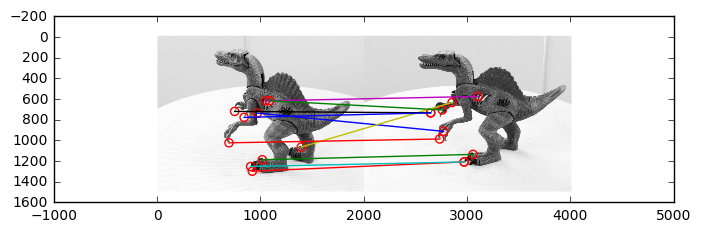
\includegraphics{fig/dinoMatch.png}

    \begin{Verbatim}[commandchars=\\\{\}]
{\color{incolor}In [{\color{incolor}161}]:} \PY{k}{def} \PY{n+nf}{naive\PYZus{}matching}\PY{p}{(}\PY{n}{img1}\PY{p}{,} \PY{n}{img2}\PY{p}{,} \PY{n}{corners1}\PY{p}{,} \PY{n}{corners2}\PY{p}{,} \PY{n}{R}\PY{p}{,} \PY{n}{NCCth}\PY{p}{)}\PY{p}{:}
              \PY{l+s+sd}{\PYZdq{}\PYZdq{}\PYZdq{}Compute NCC given two windows.}
          
          \PY{l+s+sd}{    Args:}
          \PY{l+s+sd}{        img1: Image 1.}
          \PY{l+s+sd}{        img2: Image 2.}
          \PY{l+s+sd}{        corners1: Corners in image 1 (nx2)}
          \PY{l+s+sd}{        corners2: Corners in image 2 (nx2)}
          \PY{l+s+sd}{        R: NCC matching radius}
          \PY{l+s+sd}{        NCCth: NCC matching score threshold}
          
          \PY{l+s+sd}{    Returns:}
          \PY{l+s+sd}{        NCC matching result a list of tuple (c1, c2), }
          \PY{l+s+sd}{        c1 is the 1x2 corner location in image 1, }
          \PY{l+s+sd}{        c2 is the 1x2 corner location in image 2. }
          
          \PY{l+s+sd}{    \PYZdq{}\PYZdq{}\PYZdq{}}
              
              \PY{l+s+sd}{\PYZdq{}\PYZdq{}\PYZdq{}}
          \PY{l+s+sd}{    Your code here:}
          \PY{l+s+sd}{    \PYZdq{}\PYZdq{}\PYZdq{}}
              \PY{n}{matching} \PY{o}{=} \PY{p}{[}\PY{p}{]}
              \PY{k}{for} \PY{n}{c1} \PY{o+ow}{in} \PY{n}{corners1}\PY{p}{:}
                  \PY{k}{for} \PY{n}{c2} \PY{o+ow}{in} \PY{n}{corners2}\PY{p}{:}
                      \PY{k}{if} \PY{n}{ncc\PYZus{}match}\PY{p}{(}\PY{n}{img1}\PY{p}{,} \PY{n}{img2}\PY{p}{,} \PY{n}{c1}\PY{p}{,} \PY{n}{c2}\PY{p}{,} \PY{n}{R}\PY{p}{)} \PY{o}{\PYZgt{}} \PY{n}{NCCth}\PY{p}{:}
                          \PY{n}{matching}\PY{o}{.}\PY{n}{append}\PY{p}{(}\PY{p}{(}\PY{n}{c1}\PY{p}{,} \PY{n}{c2}\PY{p}{)}\PY{p}{)}
              \PY{k}{return} \PY{n}{matching}
          
          
          \PY{c+c1}{\PYZsh{} plot matching result}
          \PY{k}{def} \PY{n+nf}{show\PYZus{}matching\PYZus{}result}\PY{p}{(}\PY{n}{img1}\PY{p}{,} \PY{n}{img2}\PY{p}{,} \PY{n}{matching}\PY{p}{)}\PY{p}{:}
              \PY{n}{fig} \PY{o}{=} \PY{n}{plt}\PY{o}{.}\PY{n}{figure}\PY{p}{(}\PY{n}{figsize}\PY{o}{=}\PY{p}{(}\PY{l+m+mi}{8}\PY{p}{,} \PY{l+m+mi}{8}\PY{p}{)}\PY{p}{)}
              \PY{n}{plt}\PY{o}{.}\PY{n}{imshow}\PY{p}{(}\PY{n}{np}\PY{o}{.}\PY{n}{hstack}\PY{p}{(}\PY{p}{(}\PY{n}{img1}\PY{p}{,} \PY{n}{img2}\PY{p}{)}\PY{p}{)}\PY{p}{,} \PY{n}{cmap}\PY{o}{=}\PY{l+s+s1}{\PYZsq{}}\PY{l+s+s1}{gray}\PY{l+s+s1}{\PYZsq{}}\PY{p}{)} \PY{c+c1}{\PYZsh{} two dino images are of different sizes, resize one before use}
              \PY{k}{for} \PY{n}{p1}\PY{p}{,} \PY{n}{p2} \PY{o+ow}{in} \PY{n}{matching}\PY{p}{:}
                  \PY{n}{plt}\PY{o}{.}\PY{n}{scatter}\PY{p}{(}\PY{n}{p1}\PY{p}{[}\PY{l+m+mi}{0}\PY{p}{]}\PY{p}{,} \PY{n}{p1}\PY{p}{[}\PY{l+m+mi}{1}\PY{p}{]}\PY{p}{,} \PY{n}{s}\PY{o}{=}\PY{l+m+mi}{35}\PY{p}{,} \PY{n}{edgecolors}\PY{o}{=}\PY{l+s+s1}{\PYZsq{}}\PY{l+s+s1}{r}\PY{l+s+s1}{\PYZsq{}}\PY{p}{,} \PY{n}{facecolors}\PY{o}{=}\PY{l+s+s1}{\PYZsq{}}\PY{l+s+s1}{none}\PY{l+s+s1}{\PYZsq{}}\PY{p}{)}
                  \PY{n}{plt}\PY{o}{.}\PY{n}{scatter}\PY{p}{(}\PY{n}{p2}\PY{p}{[}\PY{l+m+mi}{0}\PY{p}{]} \PY{o}{+} \PY{n}{img1}\PY{o}{.}\PY{n}{shape}\PY{p}{[}\PY{l+m+mi}{1}\PY{p}{]}\PY{p}{,} \PY{n}{p2}\PY{p}{[}\PY{l+m+mi}{1}\PY{p}{]}\PY{p}{,} \PY{n}{s}\PY{o}{=}\PY{l+m+mi}{35}\PY{p}{,} \PY{n}{edgecolors}\PY{o}{=}\PY{l+s+s1}{\PYZsq{}}\PY{l+s+s1}{r}\PY{l+s+s1}{\PYZsq{}}\PY{p}{,} \PY{n}{facecolors}\PY{o}{=}\PY{l+s+s1}{\PYZsq{}}\PY{l+s+s1}{none}\PY{l+s+s1}{\PYZsq{}}\PY{p}{)}
                  \PY{n}{plt}\PY{o}{.}\PY{n}{plot}\PY{p}{(}\PY{p}{[}\PY{n}{p1}\PY{p}{[}\PY{l+m+mi}{0}\PY{p}{]}\PY{p}{,} \PY{n}{p2}\PY{p}{[}\PY{l+m+mi}{0}\PY{p}{]} \PY{o}{+} \PY{n}{img1}\PY{o}{.}\PY{n}{shape}\PY{p}{[}\PY{l+m+mi}{1}\PY{p}{]}\PY{p}{]}\PY{p}{,} \PY{p}{[}\PY{n}{p1}\PY{p}{[}\PY{l+m+mi}{1}\PY{p}{]}\PY{p}{,} \PY{n}{p2}\PY{p}{[}\PY{l+m+mi}{1}\PY{p}{]}\PY{p}{]}\PY{p}{)}
              \PY{n}{plt}\PY{o}{.}\PY{n}{savefig}\PY{p}{(}\PY{l+s+s1}{\PYZsq{}}\PY{l+s+s1}{dino\PYZus{}matching.png}\PY{l+s+s1}{\PYZsq{}}\PY{p}{)}
              \PY{n}{plt}\PY{o}{.}\PY{n}{show}\PY{p}{(}\PY{p}{)}
\end{Verbatim}


    \begin{Verbatim}[commandchars=\\\{\}]
{\color{incolor}In [{\color{incolor}162}]:} \PY{n}{smoothSTD} \PY{o}{=} \PY{l+m+mi}{2}
          \PY{n}{windowSize} \PY{o}{=} \PY{l+m+mi}{11}
          \PY{n}{R} \PY{o}{=} \PY{l+m+mi}{15}
          \PY{n}{NCCth} \PY{o}{=} \PY{l+m+mf}{0.7}
\end{Verbatim}


    \begin{Verbatim}[commandchars=\\\{\}]
{\color{incolor}In [{\color{incolor}163}]:} \PY{c+c1}{\PYZsh{} detect corners on warrior and matrix sets}
          \PY{c+c1}{\PYZsh{} adjust your corner detection parameters here}
          
          \PY{k}{for} \PY{n}{nCorners} \PY{o+ow}{in} \PY{p}{[}\PY{l+m+mi}{10}\PY{p}{,} \PY{l+m+mi}{20} \PY{p}{,} \PY{l+m+mi}{30}\PY{p}{]}\PY{p}{:}
              \PY{n+nb}{print}\PY{p}{(}\PY{l+s+s1}{\PYZsq{}}\PY{l+s+s1}{number of corner is }\PY{l+s+s1}{\PYZsq{}}\PY{p}{,} \PY{n}{nCorners}\PY{p}{)}
              \PY{c+c1}{\PYZsh{} read images and detect corners on images}
              \PY{n}{imgs\PYZus{}mat} \PY{o}{=} \PY{p}{[}\PY{p}{]}
              \PY{n}{crns\PYZus{}mat} \PY{o}{=} \PY{p}{[}\PY{p}{]}
              \PY{n}{imgs\PYZus{}war} \PY{o}{=} \PY{p}{[}\PY{p}{]}
              \PY{n}{crns\PYZus{}war} \PY{o}{=} \PY{p}{[}\PY{p}{]}
              \PY{k}{for} \PY{n}{i} \PY{o+ow}{in} \PY{n+nb}{range}\PY{p}{(}\PY{l+m+mi}{2}\PY{p}{)}\PY{p}{:}
                  \PY{n}{img\PYZus{}mat} \PY{o}{=} \PY{n}{imread}\PY{p}{(}\PY{l+s+s1}{\PYZsq{}}\PY{l+s+s1}{p4/matrix/matrix}\PY{l+s+s1}{\PYZsq{}} \PY{o}{+} \PY{n+nb}{str}\PY{p}{(}\PY{n}{i}\PY{p}{)} \PY{o}{+} \PY{l+s+s1}{\PYZsq{}}\PY{l+s+s1}{.png}\PY{l+s+s1}{\PYZsq{}}\PY{p}{)}
                  \PY{n}{imgs\PYZus{}mat}\PY{o}{.}\PY{n}{append}\PY{p}{(}\PY{n}{rgb2gray}\PY{p}{(}\PY{n}{img\PYZus{}mat}\PY{p}{)}\PY{p}{)}
                  \PY{c+c1}{\PYZsh{} downsize your image in case corner\PYZus{}detect runs slow in test}
                  \PY{c+c1}{\PYZsh{} imgs\PYZus{}mat.append(rgb2gray(img\PYZus{}mat)[::2, ::2])}
                  \PY{n}{crns\PYZus{}mat}\PY{o}{.}\PY{n}{append}\PY{p}{(}\PY{n}{corner\PYZus{}detect}\PY{p}{(}\PY{n}{imgs\PYZus{}mat}\PY{p}{[}\PY{n}{i}\PY{p}{]}\PY{p}{,} \PY{n}{nCorners}\PY{p}{,} \PY{n}{smoothSTD}\PY{p}{,} \PY{n}{windowSize}\PY{p}{)}\PY{p}{)}
          
                  \PY{n}{img\PYZus{}war} \PY{o}{=} \PY{n}{imread}\PY{p}{(}\PY{l+s+s1}{\PYZsq{}}\PY{l+s+s1}{p4/warrior/warrior}\PY{l+s+s1}{\PYZsq{}} \PY{o}{+} \PY{n+nb}{str}\PY{p}{(}\PY{n}{i}\PY{p}{)} \PY{o}{+} \PY{l+s+s1}{\PYZsq{}}\PY{l+s+s1}{.png}\PY{l+s+s1}{\PYZsq{}}\PY{p}{)}
                  \PY{n}{imgs\PYZus{}war}\PY{o}{.}\PY{n}{append}\PY{p}{(}\PY{n}{rgb2gray}\PY{p}{(}\PY{n}{img\PYZus{}war}\PY{p}{)}\PY{p}{)}
                  \PY{c+c1}{\PYZsh{} downsize your image in case corner\PYZus{}detect runs slow in test}
                  \PY{c+c1}{\PYZsh{} imgs\PYZus{}war.append(rgb2gray(img\PYZus{}war)[::2, ::2])}
                  \PY{n}{crns\PYZus{}war}\PY{o}{.}\PY{n}{append}\PY{p}{(}\PY{n}{corner\PYZus{}detect}\PY{p}{(}\PY{n}{imgs\PYZus{}war}\PY{p}{[}\PY{n}{i}\PY{p}{]}\PY{p}{,} \PY{n}{nCorners}\PY{p}{,} \PY{n}{smoothSTD}\PY{p}{,} \PY{n}{windowSize}\PY{p}{)}\PY{p}{)}
          
              \PY{c+c1}{\PYZsh{} match corners}
              \PY{n}{matching\PYZus{}mat} \PY{o}{=} \PY{n}{naive\PYZus{}matching}\PY{p}{(}\PY{n}{imgs\PYZus{}mat}\PY{p}{[}\PY{l+m+mi}{0}\PY{p}{]}\PY{o}{/}\PY{l+m+mi}{255}\PY{p}{,} \PY{n}{imgs\PYZus{}mat}\PY{p}{[}\PY{l+m+mi}{1}\PY{p}{]}\PY{o}{/}\PY{l+m+mi}{255}\PY{p}{,} \PY{n}{crns\PYZus{}mat}\PY{p}{[}\PY{l+m+mi}{0}\PY{p}{]}\PY{p}{,} \PY{n}{crns\PYZus{}mat}\PY{p}{[}\PY{l+m+mi}{1}\PY{p}{]}\PY{p}{,} \PY{n}{R}\PY{p}{,} \PY{n}{NCCth}\PY{p}{)}
              \PY{n}{matching\PYZus{}war} \PY{o}{=} \PY{n}{naive\PYZus{}matching}\PY{p}{(}\PY{n}{imgs\PYZus{}war}\PY{p}{[}\PY{l+m+mi}{0}\PY{p}{]}\PY{o}{/}\PY{l+m+mi}{255}\PY{p}{,} \PY{n}{imgs\PYZus{}war}\PY{p}{[}\PY{l+m+mi}{1}\PY{p}{]}\PY{o}{/}\PY{l+m+mi}{255}\PY{p}{,} \PY{n}{crns\PYZus{}war}\PY{p}{[}\PY{l+m+mi}{0}\PY{p}{]}\PY{p}{,} \PY{n}{crns\PYZus{}war}\PY{p}{[}\PY{l+m+mi}{1}\PY{p}{]}\PY{p}{,} \PY{n}{R}\PY{p}{,} \PY{n}{NCCth}\PY{p}{)}
              \PY{n}{show\PYZus{}matching\PYZus{}result}\PY{p}{(}\PY{n}{imgs\PYZus{}mat}\PY{p}{[}\PY{l+m+mi}{0}\PY{p}{]}\PY{p}{,} \PY{n}{imgs\PYZus{}mat}\PY{p}{[}\PY{l+m+mi}{1}\PY{p}{]}\PY{p}{,} \PY{n}{matching\PYZus{}mat}\PY{p}{)}
              \PY{n}{show\PYZus{}matching\PYZus{}result}\PY{p}{(}\PY{n}{imgs\PYZus{}war}\PY{p}{[}\PY{l+m+mi}{0}\PY{p}{]}\PY{p}{,} \PY{n}{imgs\PYZus{}war}\PY{p}{[}\PY{l+m+mi}{1}\PY{p}{]}\PY{p}{,} \PY{n}{matching\PYZus{}war}\PY{p}{)}
              \PY{n+nb}{print}\PY{p}{(}\PY{l+s+s1}{\PYZsq{}}\PY{l+s+se}{\PYZbs{}n}\PY{l+s+s1}{\PYZsq{}}\PY{p}{)}
\end{Verbatim}


    \begin{Verbatim}[commandchars=\\\{\}]
number of corner is  10

    \end{Verbatim}

    \begin{Verbatim}[commandchars=\\\{\}]
/usr/local/lib/python3.7/site-packages/ipykernel\_launcher.py:12: DeprecationWarning: `imread` is deprecated!
`imread` is deprecated in SciPy 1.0.0, and will be removed in 1.2.0.
Use ``imageio.imread`` instead.
  if sys.path[0] == '':
/usr/local/lib/python3.7/site-packages/ipykernel\_launcher.py:18: DeprecationWarning: `imread` is deprecated!
`imread` is deprecated in SciPy 1.0.0, and will be removed in 1.2.0.
Use ``imageio.imread`` instead.

    \end{Verbatim}

    \begin{center}
    \adjustimage{max size={0.9\linewidth}{0.9\paperheight}}{output_19_2.png}
    \end{center}
    { \hspace*{\fill} \\}
    
    \begin{center}
    \adjustimage{max size={0.9\linewidth}{0.9\paperheight}}{output_19_3.png}
    \end{center}
    { \hspace*{\fill} \\}
    
    \begin{Verbatim}[commandchars=\\\{\}]


number of corner is  20

    \end{Verbatim}

    \begin{center}
    \adjustimage{max size={0.9\linewidth}{0.9\paperheight}}{output_19_5.png}
    \end{center}
    { \hspace*{\fill} \\}
    
    \begin{center}
    \adjustimage{max size={0.9\linewidth}{0.9\paperheight}}{output_19_6.png}
    \end{center}
    { \hspace*{\fill} \\}
    
    \begin{Verbatim}[commandchars=\\\{\}]


number of corner is  30

    \end{Verbatim}

    \begin{center}
    \adjustimage{max size={0.9\linewidth}{0.9\paperheight}}{output_19_8.png}
    \end{center}
    { \hspace*{\fill} \\}
    
    \begin{center}
    \adjustimage{max size={0.9\linewidth}{0.9\paperheight}}{output_19_9.png}
    \end{center}
    { \hspace*{\fill} \\}
    
    \begin{Verbatim}[commandchars=\\\{\}]



    \end{Verbatim}

    \hypertarget{epipolar-geometry-4-pts}{%
\subsubsection{Epipolar Geometry {[}4
pts{]}}\label{epipolar-geometry-4-pts}}

Using the fundamental\_matrix function, and the corresponding points
provided in cor1.npy and cor2.npy, calculate the fundamental matrix.

Using this fundamental matrix, plot the epipolar lines in both image
pairs across all images. For this part you may want to complete the
function plot\_epipolar\_lines. Shown your result for matrix and warrior
as the figure below. 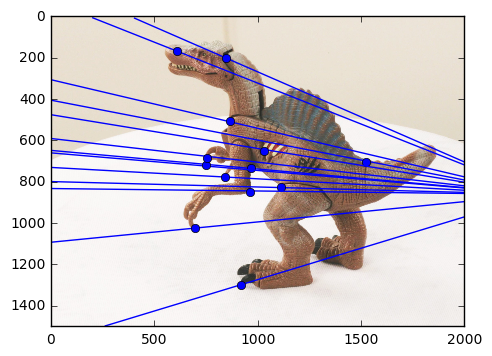
\includegraphics{fig/dinoEpi1.png}
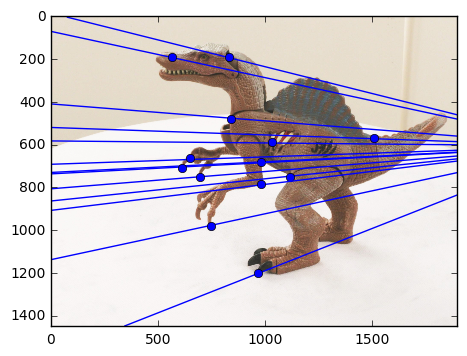
\includegraphics{fig/dinoEpi2.png}

Also, write the script to calculate the epipoles for a given Fundamental
matrix and corner point correspondences in the two images.

    \begin{Verbatim}[commandchars=\\\{\}]
{\color{incolor}In [{\color{incolor}46}]:} \PY{c+c1}{\PYZsh{}\PYZsh{} import numpy as np}
         \PY{k+kn}{from} \PY{n+nn}{scipy}\PY{n+nn}{.}\PY{n+nn}{misc} \PY{k}{import} \PY{n}{imread}
         \PY{k+kn}{import} \PY{n+nn}{matplotlib}\PY{n+nn}{.}\PY{n+nn}{pyplot} \PY{k}{as} \PY{n+nn}{plt}
         \PY{k+kn}{from} \PY{n+nn}{scipy}\PY{n+nn}{.}\PY{n+nn}{io} \PY{k}{import} \PY{n}{loadmat}
         
         \PY{k}{def} \PY{n+nf}{compute\PYZus{}fundamental}\PY{p}{(}\PY{n}{x1}\PY{p}{,}\PY{n}{x2}\PY{p}{)}\PY{p}{:}
             \PY{l+s+sd}{\PYZdq{}\PYZdq{}\PYZdq{}    Computes the fundamental matrix from corresponding points }
         \PY{l+s+sd}{        (x1,x2 3*n arrays) using the 8 point algorithm.}
         \PY{l+s+sd}{        Each row in the A matrix below is constructed as}
         \PY{l+s+sd}{        [x\PYZsq{}*x, x\PYZsq{}*y, x\PYZsq{}, y\PYZsq{}*x, y\PYZsq{}*y, y\PYZsq{}, x, y, 1] }
         \PY{l+s+sd}{    \PYZdq{}\PYZdq{}\PYZdq{}}
             
             \PY{n}{n} \PY{o}{=} \PY{n}{x1}\PY{o}{.}\PY{n}{shape}\PY{p}{[}\PY{l+m+mi}{1}\PY{p}{]}
             \PY{k}{if} \PY{n}{x2}\PY{o}{.}\PY{n}{shape}\PY{p}{[}\PY{l+m+mi}{1}\PY{p}{]} \PY{o}{!=} \PY{n}{n}\PY{p}{:}
                 \PY{k}{raise} \PY{n+ne}{ValueError}\PY{p}{(}\PY{l+s+s2}{\PYZdq{}}\PY{l+s+s2}{Number of points don}\PY{l+s+s2}{\PYZsq{}}\PY{l+s+s2}{t match.}\PY{l+s+s2}{\PYZdq{}}\PY{p}{)}
             
             \PY{c+c1}{\PYZsh{} build matrix for equations}
             \PY{n}{A} \PY{o}{=} \PY{n}{np}\PY{o}{.}\PY{n}{zeros}\PY{p}{(}\PY{p}{(}\PY{n}{n}\PY{p}{,}\PY{l+m+mi}{9}\PY{p}{)}\PY{p}{)}
             \PY{k}{for} \PY{n}{i} \PY{o+ow}{in} \PY{n+nb}{range}\PY{p}{(}\PY{n}{n}\PY{p}{)}\PY{p}{:}
                 \PY{n}{A}\PY{p}{[}\PY{n}{i}\PY{p}{]} \PY{o}{=} \PY{p}{[}\PY{n}{x1}\PY{p}{[}\PY{l+m+mi}{0}\PY{p}{,}\PY{n}{i}\PY{p}{]}\PY{o}{*}\PY{n}{x2}\PY{p}{[}\PY{l+m+mi}{0}\PY{p}{,}\PY{n}{i}\PY{p}{]}\PY{p}{,} \PY{n}{x1}\PY{p}{[}\PY{l+m+mi}{0}\PY{p}{,}\PY{n}{i}\PY{p}{]}\PY{o}{*}\PY{n}{x2}\PY{p}{[}\PY{l+m+mi}{1}\PY{p}{,}\PY{n}{i}\PY{p}{]}\PY{p}{,} \PY{n}{x1}\PY{p}{[}\PY{l+m+mi}{0}\PY{p}{,}\PY{n}{i}\PY{p}{]}\PY{o}{*}\PY{n}{x2}\PY{p}{[}\PY{l+m+mi}{2}\PY{p}{,}\PY{n}{i}\PY{p}{]}\PY{p}{,}
                         \PY{n}{x1}\PY{p}{[}\PY{l+m+mi}{1}\PY{p}{,}\PY{n}{i}\PY{p}{]}\PY{o}{*}\PY{n}{x2}\PY{p}{[}\PY{l+m+mi}{0}\PY{p}{,}\PY{n}{i}\PY{p}{]}\PY{p}{,} \PY{n}{x1}\PY{p}{[}\PY{l+m+mi}{1}\PY{p}{,}\PY{n}{i}\PY{p}{]}\PY{o}{*}\PY{n}{x2}\PY{p}{[}\PY{l+m+mi}{1}\PY{p}{,}\PY{n}{i}\PY{p}{]}\PY{p}{,} \PY{n}{x1}\PY{p}{[}\PY{l+m+mi}{1}\PY{p}{,}\PY{n}{i}\PY{p}{]}\PY{o}{*}\PY{n}{x2}\PY{p}{[}\PY{l+m+mi}{2}\PY{p}{,}\PY{n}{i}\PY{p}{]}\PY{p}{,}
                         \PY{n}{x1}\PY{p}{[}\PY{l+m+mi}{2}\PY{p}{,}\PY{n}{i}\PY{p}{]}\PY{o}{*}\PY{n}{x2}\PY{p}{[}\PY{l+m+mi}{0}\PY{p}{,}\PY{n}{i}\PY{p}{]}\PY{p}{,} \PY{n}{x1}\PY{p}{[}\PY{l+m+mi}{2}\PY{p}{,}\PY{n}{i}\PY{p}{]}\PY{o}{*}\PY{n}{x2}\PY{p}{[}\PY{l+m+mi}{1}\PY{p}{,}\PY{n}{i}\PY{p}{]}\PY{p}{,} \PY{n}{x1}\PY{p}{[}\PY{l+m+mi}{2}\PY{p}{,}\PY{n}{i}\PY{p}{]}\PY{o}{*}\PY{n}{x2}\PY{p}{[}\PY{l+m+mi}{2}\PY{p}{,}\PY{n}{i}\PY{p}{]} \PY{p}{]}
                     
             \PY{c+c1}{\PYZsh{} compute linear least square solution}
             \PY{n}{U}\PY{p}{,}\PY{n}{S}\PY{p}{,}\PY{n}{V} \PY{o}{=} \PY{n}{np}\PY{o}{.}\PY{n}{linalg}\PY{o}{.}\PY{n}{svd}\PY{p}{(}\PY{n}{A}\PY{p}{)}
             \PY{n}{F} \PY{o}{=} \PY{n}{V}\PY{p}{[}\PY{o}{\PYZhy{}}\PY{l+m+mi}{1}\PY{p}{]}\PY{o}{.}\PY{n}{reshape}\PY{p}{(}\PY{l+m+mi}{3}\PY{p}{,}\PY{l+m+mi}{3}\PY{p}{)} \PY{c+c1}{\PYZsh{} minimum eigen value}
             
                 
             \PY{c+c1}{\PYZsh{} constrain F}
             \PY{c+c1}{\PYZsh{} make rank 2 by zeroing out last singular value}
             \PY{n}{U}\PY{p}{,}\PY{n}{S}\PY{p}{,}\PY{n}{V} \PY{o}{=} \PY{n}{np}\PY{o}{.}\PY{n}{linalg}\PY{o}{.}\PY{n}{svd}\PY{p}{(}\PY{n}{F}\PY{p}{)}
             \PY{n}{S}\PY{p}{[}\PY{l+m+mi}{2}\PY{p}{]} \PY{o}{=} \PY{l+m+mi}{0}
             \PY{n}{F} \PY{o}{=} \PY{n}{np}\PY{o}{.}\PY{n}{dot}\PY{p}{(}\PY{n}{U}\PY{p}{,}\PY{n}{np}\PY{o}{.}\PY{n}{dot}\PY{p}{(}\PY{n}{np}\PY{o}{.}\PY{n}{diag}\PY{p}{(}\PY{n}{S}\PY{p}{)}\PY{p}{,}\PY{n}{V}\PY{p}{)}\PY{p}{)}
             
             \PY{k}{return} \PY{n}{F}\PY{o}{/}\PY{n}{F}\PY{p}{[}\PY{l+m+mi}{2}\PY{p}{,}\PY{l+m+mi}{2}\PY{p}{]}
         
         
         \PY{k}{def} \PY{n+nf}{fundamental\PYZus{}matrix}\PY{p}{(}\PY{n}{x1}\PY{p}{,}\PY{n}{x2}\PY{p}{)}\PY{p}{:}
             \PY{c+c1}{\PYZsh{}3*n}
             \PY{n}{n} \PY{o}{=} \PY{n}{x1}\PY{o}{.}\PY{n}{shape}\PY{p}{[}\PY{l+m+mi}{1}\PY{p}{]}
             \PY{k}{if} \PY{n}{x2}\PY{o}{.}\PY{n}{shape}\PY{p}{[}\PY{l+m+mi}{1}\PY{p}{]} \PY{o}{!=} \PY{n}{n}\PY{p}{:}
                 \PY{k}{raise} \PY{n+ne}{ValueError}\PY{p}{(}\PY{l+s+s2}{\PYZdq{}}\PY{l+s+s2}{Number of points don}\PY{l+s+s2}{\PYZsq{}}\PY{l+s+s2}{t match.}\PY{l+s+s2}{\PYZdq{}}\PY{p}{)}
         
             \PY{c+c1}{\PYZsh{} normalize image coordinates}
             \PY{n}{x1} \PY{o}{=} \PY{n}{x1} \PY{o}{/} \PY{n}{x1}\PY{p}{[}\PY{l+m+mi}{2}\PY{p}{]}
             \PY{n}{mean\PYZus{}1} \PY{o}{=} \PY{n}{np}\PY{o}{.}\PY{n}{mean}\PY{p}{(}\PY{n}{x1}\PY{p}{[}\PY{p}{:}\PY{l+m+mi}{2}\PY{p}{]}\PY{p}{,}\PY{n}{axis}\PY{o}{=}\PY{l+m+mi}{1}\PY{p}{)}
             \PY{n}{S1} \PY{o}{=} \PY{n}{np}\PY{o}{.}\PY{n}{sqrt}\PY{p}{(}\PY{l+m+mi}{2}\PY{p}{)} \PY{o}{/} \PY{n}{np}\PY{o}{.}\PY{n}{std}\PY{p}{(}\PY{n}{x1}\PY{p}{[}\PY{p}{:}\PY{l+m+mi}{2}\PY{p}{]}\PY{p}{)}
             \PY{n}{T1} \PY{o}{=} \PY{n}{np}\PY{o}{.}\PY{n}{array}\PY{p}{(}\PY{p}{[}\PY{p}{[}\PY{n}{S1}\PY{p}{,}\PY{l+m+mi}{0}\PY{p}{,}\PY{o}{\PYZhy{}}\PY{n}{S1}\PY{o}{*}\PY{n}{mean\PYZus{}1}\PY{p}{[}\PY{l+m+mi}{0}\PY{p}{]}\PY{p}{]}\PY{p}{,}\PY{p}{[}\PY{l+m+mi}{0}\PY{p}{,}\PY{n}{S1}\PY{p}{,}\PY{o}{\PYZhy{}}\PY{n}{S1}\PY{o}{*}\PY{n}{mean\PYZus{}1}\PY{p}{[}\PY{l+m+mi}{1}\PY{p}{]}\PY{p}{]}\PY{p}{,}\PY{p}{[}\PY{l+m+mi}{0}\PY{p}{,}\PY{l+m+mi}{0}\PY{p}{,}\PY{l+m+mi}{1}\PY{p}{]}\PY{p}{]}\PY{p}{)}
             \PY{n}{x1} \PY{o}{=} \PY{n}{np}\PY{o}{.}\PY{n}{dot}\PY{p}{(}\PY{n}{T1}\PY{p}{,}\PY{n}{x1}\PY{p}{)}
             
             \PY{n}{x2} \PY{o}{=} \PY{n}{x2} \PY{o}{/} \PY{n}{x2}\PY{p}{[}\PY{l+m+mi}{2}\PY{p}{]}
             \PY{n}{mean\PYZus{}2} \PY{o}{=} \PY{n}{np}\PY{o}{.}\PY{n}{mean}\PY{p}{(}\PY{n}{x2}\PY{p}{[}\PY{p}{:}\PY{l+m+mi}{2}\PY{p}{]}\PY{p}{,}\PY{n}{axis}\PY{o}{=}\PY{l+m+mi}{1}\PY{p}{)}
             \PY{n}{S2} \PY{o}{=} \PY{n}{np}\PY{o}{.}\PY{n}{sqrt}\PY{p}{(}\PY{l+m+mi}{2}\PY{p}{)} \PY{o}{/} \PY{n}{np}\PY{o}{.}\PY{n}{std}\PY{p}{(}\PY{n}{x2}\PY{p}{[}\PY{p}{:}\PY{l+m+mi}{2}\PY{p}{]}\PY{p}{)}
             \PY{n}{T2} \PY{o}{=} \PY{n}{np}\PY{o}{.}\PY{n}{array}\PY{p}{(}\PY{p}{[}\PY{p}{[}\PY{n}{S2}\PY{p}{,}\PY{l+m+mi}{0}\PY{p}{,}\PY{o}{\PYZhy{}}\PY{n}{S2}\PY{o}{*}\PY{n}{mean\PYZus{}2}\PY{p}{[}\PY{l+m+mi}{0}\PY{p}{]}\PY{p}{]}\PY{p}{,}\PY{p}{[}\PY{l+m+mi}{0}\PY{p}{,}\PY{n}{S2}\PY{p}{,}\PY{o}{\PYZhy{}}\PY{n}{S2}\PY{o}{*}\PY{n}{mean\PYZus{}2}\PY{p}{[}\PY{l+m+mi}{1}\PY{p}{]}\PY{p}{]}\PY{p}{,}\PY{p}{[}\PY{l+m+mi}{0}\PY{p}{,}\PY{l+m+mi}{0}\PY{p}{,}\PY{l+m+mi}{1}\PY{p}{]}\PY{p}{]}\PY{p}{)}
             \PY{n}{x2} \PY{o}{=} \PY{n}{np}\PY{o}{.}\PY{n}{dot}\PY{p}{(}\PY{n}{T2}\PY{p}{,}\PY{n}{x2}\PY{p}{)}
         
             \PY{c+c1}{\PYZsh{} compute F with the normalized coordinates}
             \PY{n}{F} \PY{o}{=} \PY{n}{compute\PYZus{}fundamental}\PY{p}{(}\PY{n}{x1}\PY{p}{,}\PY{n}{x2}\PY{p}{)}
         
             \PY{c+c1}{\PYZsh{} reverse normalization}
             \PY{n}{F} \PY{o}{=} \PY{n}{np}\PY{o}{.}\PY{n}{dot}\PY{p}{(}\PY{n}{T1}\PY{o}{.}\PY{n}{T}\PY{p}{,}\PY{n}{np}\PY{o}{.}\PY{n}{dot}\PY{p}{(}\PY{n}{F}\PY{p}{,}\PY{n}{T2}\PY{p}{)}\PY{p}{)}
         
             \PY{k}{return} \PY{n}{F}\PY{o}{/}\PY{n}{F}\PY{p}{[}\PY{l+m+mi}{2}\PY{p}{,}\PY{l+m+mi}{2}\PY{p}{]}
         
         
         \PY{k}{def} \PY{n+nf}{compute\PYZus{}epipole}\PY{p}{(}\PY{n}{F}\PY{p}{)}\PY{p}{:}
             \PY{l+s+sd}{\PYZsq{}\PYZsq{}\PYZsq{}}
         \PY{l+s+sd}{    This function computes the epipoles for a given fundamental matrix and corner point correspondences}
         \PY{l+s+sd}{    input:}
         \PY{l+s+sd}{    F\PYZhy{}\PYZhy{}\PYZgt{} Fundamental matrix}
         \PY{l+s+sd}{    output:}
         \PY{l+s+sd}{    e1\PYZhy{}\PYZhy{}\PYZgt{} corresponding epipole in image 1}
         \PY{l+s+sd}{    e2\PYZhy{}\PYZhy{}\PYZgt{} epipole in image2}
         \PY{l+s+sd}{    \PYZsq{}\PYZsq{}\PYZsq{}}
             \PY{c+c1}{\PYZsh{}your code here}
             
             
         \PY{c+c1}{\PYZsh{}     e1\PYZus{}lmbds, e1\PYZus{}egnvctrs = np.linalg.eig(F.T)}
         \PY{c+c1}{\PYZsh{}     e1\PYZus{}idx = np.argmin(abs(e1\PYZus{}lmbds))}
         \PY{c+c1}{\PYZsh{}     e1 = e1\PYZus{}egnvctrs[:, e1\PYZus{}idx]}
             
         \PY{c+c1}{\PYZsh{}     e2\PYZus{}lmbds, egnvctrs = np.linalg.eig(F)}
         \PY{c+c1}{\PYZsh{}     e2\PYZus{}idx = np.argmin(abs(e2\PYZus{}lmbds))}
         \PY{c+c1}{\PYZsh{}     e2 = e1\PYZus{}egnvctrs[:, e2\PYZus{}idx]}
             \PY{n}{U}\PY{p}{,}\PY{n}{S}\PY{p}{,}\PY{n}{Vh} \PY{o}{=} \PY{n}{np}\PY{o}{.}\PY{n}{linalg}\PY{o}{.}\PY{n}{svd}\PY{p}{(}\PY{n}{F}\PY{p}{)}
             \PY{c+c1}{\PYZsh{} e2 is last column of V}
             \PY{c+c1}{\PYZsh{} e1 is last column of U}
             \PY{n}{e1} \PY{o}{=} \PY{n}{U}\PY{p}{[}\PY{p}{:}\PY{p}{,} \PY{o}{\PYZhy{}}\PY{l+m+mi}{1}\PY{p}{]}
             \PY{n}{e2} \PY{o}{=} \PY{n}{Vh}\PY{p}{[}\PY{o}{\PYZhy{}}\PY{l+m+mi}{1}\PY{p}{]}
             
             \PY{n}{e1} \PY{o}{=} \PY{n}{e1}\PY{o}{/}\PY{n}{e1}\PY{p}{[}\PY{o}{\PYZhy{}}\PY{l+m+mi}{1}\PY{p}{]}
             \PY{n}{e2} \PY{o}{=} \PY{n}{e2}\PY{o}{/}\PY{n}{e2}\PY{p}{[}\PY{o}{\PYZhy{}}\PY{l+m+mi}{1}\PY{p}{]}
             
             \PY{k}{return} \PY{n}{e1}\PY{p}{,} \PY{n}{e2}
\end{Verbatim}


    \begin{Verbatim}[commandchars=\\\{\}]
{\color{incolor}In [{\color{incolor}47}]:} \PY{k}{def} \PY{n+nf}{plot\PYZus{}epipolar\PYZus{}lines}\PY{p}{(}\PY{n}{img1}\PY{p}{,}\PY{n}{img2}\PY{p}{,} \PY{n}{cor1}\PY{p}{,} \PY{n}{cor2}\PY{p}{)}\PY{p}{:}
             \PY{l+s+sd}{\PYZdq{}\PYZdq{}\PYZdq{}Plot epipolar lines on image given image, corners}
         
         \PY{l+s+sd}{    Args:}
         \PY{l+s+sd}{        img1: Image 1.}
         \PY{l+s+sd}{        img2: Image 2.}
         \PY{l+s+sd}{        cor1: Corners in homogeneous image coordinate in image 1 (3xn)}
         \PY{l+s+sd}{        cor2: Corners in homogeneous image coordinate in image 2 (3xn)}
         
         \PY{l+s+sd}{    \PYZdq{}\PYZdq{}\PYZdq{}}
             
             \PY{l+s+sd}{\PYZdq{}\PYZdq{}\PYZdq{}}
         \PY{l+s+sd}{    Your code here:}
         \PY{l+s+sd}{    \PYZdq{}\PYZdq{}\PYZdq{}}
             \PY{n}{F} \PY{o}{=} \PY{n}{fundamental\PYZus{}matrix}\PY{p}{(}\PY{n}{cor1}\PY{p}{,}\PY{n}{cor2}\PY{p}{)}
             \PY{n}{lines1} \PY{o}{=} \PY{n}{np}\PY{o}{.}\PY{n}{dot}\PY{p}{(}\PY{n}{F}\PY{p}{,}\PY{n}{cor2}\PY{p}{)}
             \PY{n}{lines2} \PY{o}{=} \PY{n}{np}\PY{o}{.}\PY{n}{dot}\PY{p}{(}\PY{n}{F}\PY{o}{.}\PY{n}{T}\PY{p}{,}\PY{n}{cor1}\PY{p}{)}
             
             \PY{n}{fig} \PY{o}{=} \PY{n}{plt}\PY{o}{.}\PY{n}{figure}\PY{p}{(}\PY{n}{figsize}\PY{o}{=}\PY{p}{(}\PY{l+m+mi}{8}\PY{p}{,} \PY{l+m+mi}{8}\PY{p}{)}\PY{p}{)}
             \PY{n}{plt}\PY{o}{.}\PY{n}{imshow}\PY{p}{(}\PY{n}{img1}\PY{p}{,} \PY{n}{cmap} \PY{o}{=} \PY{l+s+s1}{\PYZsq{}}\PY{l+s+s1}{gray}\PY{l+s+s1}{\PYZsq{}}\PY{p}{)}
         \PY{c+c1}{\PYZsh{}     for i in range(cor2.shape[1]):}
             \PY{n}{x0} \PY{o}{=} \PY{l+m+mi}{0}
             \PY{n}{y0} \PY{o}{=} \PY{o}{\PYZhy{}}\PY{n}{lines1}\PY{p}{[}\PY{l+m+mi}{2}\PY{p}{]}\PY{o}{/}\PY{n}{lines1}\PY{p}{[}\PY{l+m+mi}{1}\PY{p}{]}
         
             \PY{n}{x1} \PY{o}{=} \PY{n}{img1}\PY{o}{.}\PY{n}{shape}\PY{p}{[}\PY{l+m+mi}{1}\PY{p}{]}
             \PY{n}{y1} \PY{o}{=} \PY{o}{\PYZhy{}}\PY{n}{lines1}\PY{p}{[}\PY{l+m+mi}{0}\PY{p}{]}\PY{o}{/}\PY{n}{lines1}\PY{p}{[}\PY{l+m+mi}{1}\PY{p}{]}\PY{o}{*}\PY{n}{x1} \PY{o}{\PYZhy{}} \PY{n}{lines1}\PY{p}{[}\PY{l+m+mi}{2}\PY{p}{]}\PY{o}{/}\PY{n}{lines1}\PY{p}{[}\PY{l+m+mi}{1}\PY{p}{]}
         
             \PY{n}{plt}\PY{o}{.}\PY{n}{plot}\PY{p}{(}\PY{p}{[}\PY{n}{x0}\PY{p}{,}\PY{n}{x1}\PY{p}{]}\PY{p}{,}\PY{p}{[}\PY{n}{y0}\PY{p}{,}\PY{n}{y1}\PY{p}{]}\PY{p}{,}\PY{n}{color}\PY{o}{=}\PY{l+s+s1}{\PYZsq{}}\PY{l+s+s1}{b}\PY{l+s+s1}{\PYZsq{}}\PY{p}{)}
             \PY{n}{plt}\PY{o}{.}\PY{n}{axis}\PY{p}{(}\PY{p}{[}\PY{l+m+mi}{0}\PY{p}{,}\PY{n}{img1}\PY{o}{.}\PY{n}{shape}\PY{p}{[}\PY{l+m+mi}{1}\PY{p}{]}\PY{p}{,}\PY{n}{img1}\PY{o}{.}\PY{n}{shape}\PY{p}{[}\PY{l+m+mi}{0}\PY{p}{]}\PY{p}{,}\PY{l+m+mi}{0}\PY{p}{]}\PY{p}{)}
             \PY{n}{plt}\PY{o}{.}\PY{n}{scatter}\PY{p}{(}\PY{n}{cor1}\PY{p}{[}\PY{l+m+mi}{0}\PY{p}{,}\PY{p}{:}\PY{p}{]}\PY{p}{,}\PY{n}{cor1}\PY{p}{[}\PY{l+m+mi}{1}\PY{p}{,}\PY{p}{:}\PY{p}{]}\PY{p}{,}\PY{n}{s}\PY{o}{=}\PY{l+m+mi}{45}\PY{p}{,}\PY{n}{edgecolors}\PY{o}{=}\PY{l+s+s1}{\PYZsq{}}\PY{l+s+s1}{g}\PY{l+s+s1}{\PYZsq{}}\PY{p}{,}\PY{n}{facecolors}\PY{o}{=}\PY{l+s+s1}{\PYZsq{}}\PY{l+s+s1}{b}\PY{l+s+s1}{\PYZsq{}}\PY{p}{)}
             \PY{n}{plt}\PY{o}{.}\PY{n}{show}\PY{p}{(}\PY{p}{)}
             
             
             
             \PY{n}{fig} \PY{o}{=} \PY{n}{plt}\PY{o}{.}\PY{n}{figure}\PY{p}{(}\PY{n}{figsize}\PY{o}{=}\PY{p}{(}\PY{l+m+mi}{8}\PY{p}{,} \PY{l+m+mi}{8}\PY{p}{)}\PY{p}{)}
             \PY{n}{plt}\PY{o}{.}\PY{n}{imshow}\PY{p}{(}\PY{n}{img2}\PY{p}{,} \PY{n}{cmap} \PY{o}{=} \PY{l+s+s1}{\PYZsq{}}\PY{l+s+s1}{gray}\PY{l+s+s1}{\PYZsq{}}\PY{p}{)}
         \PY{c+c1}{\PYZsh{}     for i in range(cor1.shape[1]):}
             \PY{n}{x0} \PY{o}{=} \PY{l+m+mi}{0}
             \PY{n}{y0} \PY{o}{=} \PY{o}{\PYZhy{}}\PY{n}{lines2}\PY{p}{[}\PY{l+m+mi}{2}\PY{p}{]}\PY{o}{/}\PY{n}{lines2}\PY{p}{[}\PY{l+m+mi}{1}\PY{p}{]}
         
             \PY{n}{x1} \PY{o}{=} \PY{n}{img1}\PY{o}{.}\PY{n}{shape}\PY{p}{[}\PY{l+m+mi}{1}\PY{p}{]}
             \PY{n}{y1} \PY{o}{=} \PY{o}{\PYZhy{}}\PY{n}{lines2}\PY{p}{[}\PY{l+m+mi}{0}\PY{p}{]}\PY{o}{/}\PY{n}{lines2}\PY{p}{[}\PY{l+m+mi}{1}\PY{p}{]}\PY{o}{*}\PY{n}{x1} \PY{o}{\PYZhy{}} \PY{n}{lines2}\PY{p}{[}\PY{l+m+mi}{2}\PY{p}{]}\PY{o}{/}\PY{n}{lines2}\PY{p}{[}\PY{l+m+mi}{1}\PY{p}{]}
         
             \PY{n}{plt}\PY{o}{.}\PY{n}{plot}\PY{p}{(}\PY{p}{[}\PY{n}{x0}\PY{p}{,}\PY{n}{x1}\PY{p}{]}\PY{p}{,}\PY{p}{[}\PY{n}{y0}\PY{p}{,}\PY{n}{y1}\PY{p}{]}\PY{p}{,}\PY{n}{color}\PY{o}{=}\PY{l+s+s1}{\PYZsq{}}\PY{l+s+s1}{b}\PY{l+s+s1}{\PYZsq{}}\PY{p}{)}
             \PY{n}{plt}\PY{o}{.}\PY{n}{axis}\PY{p}{(}\PY{p}{[}\PY{l+m+mi}{0}\PY{p}{,}\PY{n}{img2}\PY{o}{.}\PY{n}{shape}\PY{p}{[}\PY{l+m+mi}{1}\PY{p}{]}\PY{p}{,}\PY{n}{img2}\PY{o}{.}\PY{n}{shape}\PY{p}{[}\PY{l+m+mi}{0}\PY{p}{]}\PY{p}{,}\PY{l+m+mi}{0}\PY{p}{]}\PY{p}{)}
             \PY{n}{plt}\PY{o}{.}\PY{n}{scatter}\PY{p}{(}\PY{n}{cor2}\PY{p}{[}\PY{l+m+mi}{0}\PY{p}{,}\PY{p}{:}\PY{p}{]}\PY{p}{,}\PY{n}{cor2}\PY{p}{[}\PY{l+m+mi}{1}\PY{p}{,}\PY{p}{:}\PY{p}{]}\PY{p}{,}\PY{n}{s}\PY{o}{=}\PY{l+m+mi}{45}\PY{p}{,}\PY{n}{edgecolors}\PY{o}{=}\PY{l+s+s1}{\PYZsq{}}\PY{l+s+s1}{g}\PY{l+s+s1}{\PYZsq{}}\PY{p}{,}\PY{n}{facecolors}\PY{o}{=}\PY{l+s+s1}{\PYZsq{}}\PY{l+s+s1}{b}\PY{l+s+s1}{\PYZsq{}}\PY{p}{)}
             \PY{n}{plt}\PY{o}{.}\PY{n}{show}\PY{p}{(}\PY{p}{)}
         
                 
                   
\end{Verbatim}


    \begin{Verbatim}[commandchars=\\\{\}]
{\color{incolor}In [{\color{incolor}164}]:} \PY{c+c1}{\PYZsh{} replace images and corners with those of matrix and warrior}
          \PY{n}{I1} \PY{o}{=} \PY{n}{imread}\PY{p}{(}\PY{l+s+s2}{\PYZdq{}}\PY{l+s+s2}{./p4/matrix/matrix0.png}\PY{l+s+s2}{\PYZdq{}}\PY{p}{)}
          \PY{n}{I2} \PY{o}{=} \PY{n}{imread}\PY{p}{(}\PY{l+s+s2}{\PYZdq{}}\PY{l+s+s2}{./p4/matrix/matrix1.png}\PY{l+s+s2}{\PYZdq{}}\PY{p}{)}
          
          \PY{n}{cor1} \PY{o}{=} \PY{n}{np}\PY{o}{.}\PY{n}{load}\PY{p}{(}\PY{l+s+s2}{\PYZdq{}}\PY{l+s+s2}{./p4/matrix/cor1.npy}\PY{l+s+s2}{\PYZdq{}}\PY{p}{)}
          \PY{n}{cor2} \PY{o}{=} \PY{n}{np}\PY{o}{.}\PY{n}{load}\PY{p}{(}\PY{l+s+s2}{\PYZdq{}}\PY{l+s+s2}{./p4/matrix/cor2.npy}\PY{l+s+s2}{\PYZdq{}}\PY{p}{)}
          
          \PY{n}{plot\PYZus{}epipolar\PYZus{}lines}\PY{p}{(}\PY{n}{I1}\PY{p}{,}\PY{n}{I2}\PY{p}{,}\PY{n}{cor1}\PY{p}{,}\PY{n}{cor2}\PY{p}{)}
\end{Verbatim}


    \begin{Verbatim}[commandchars=\\\{\}]
/usr/local/lib/python3.7/site-packages/ipykernel\_launcher.py:2: DeprecationWarning: `imread` is deprecated!
`imread` is deprecated in SciPy 1.0.0, and will be removed in 1.2.0.
Use ``imageio.imread`` instead.
  
/usr/local/lib/python3.7/site-packages/ipykernel\_launcher.py:3: DeprecationWarning: `imread` is deprecated!
`imread` is deprecated in SciPy 1.0.0, and will be removed in 1.2.0.
Use ``imageio.imread`` instead.
  This is separate from the ipykernel package so we can avoid doing imports until

    \end{Verbatim}

    \begin{center}
    \adjustimage{max size={0.9\linewidth}{0.9\paperheight}}{output_23_1.png}
    \end{center}
    { \hspace*{\fill} \\}
    
    \begin{center}
    \adjustimage{max size={0.9\linewidth}{0.9\paperheight}}{output_23_2.png}
    \end{center}
    { \hspace*{\fill} \\}
    
    \begin{Verbatim}[commandchars=\\\{\}]
{\color{incolor}In [{\color{incolor}194}]:} \PY{c+c1}{\PYZsh{} replace images and corners with those of matrix and warrior}
          \PY{n}{I1} \PY{o}{=} \PY{n}{imread}\PY{p}{(}\PY{l+s+s2}{\PYZdq{}}\PY{l+s+s2}{./p4/warrior/warrior0.png}\PY{l+s+s2}{\PYZdq{}}\PY{p}{)}
          \PY{n}{I2} \PY{o}{=} \PY{n}{imread}\PY{p}{(}\PY{l+s+s2}{\PYZdq{}}\PY{l+s+s2}{./p4/warrior/warrior1.png}\PY{l+s+s2}{\PYZdq{}}\PY{p}{)}
          
          \PY{n}{cor1} \PY{o}{=} \PY{n}{np}\PY{o}{.}\PY{n}{load}\PY{p}{(}\PY{l+s+s2}{\PYZdq{}}\PY{l+s+s2}{./p4/warrior/cor1.npy}\PY{l+s+s2}{\PYZdq{}}\PY{p}{)}
          \PY{n}{cor2} \PY{o}{=} \PY{n}{np}\PY{o}{.}\PY{n}{load}\PY{p}{(}\PY{l+s+s2}{\PYZdq{}}\PY{l+s+s2}{./p4/warrior/cor2.npy}\PY{l+s+s2}{\PYZdq{}}\PY{p}{)}
          
          \PY{n}{plot\PYZus{}epipolar\PYZus{}lines}\PY{p}{(}\PY{n}{I1}\PY{p}{,}\PY{n}{I2}\PY{p}{,}\PY{n}{cor1}\PY{p}{,}\PY{n}{cor2}\PY{p}{)}
\end{Verbatim}


    \begin{Verbatim}[commandchars=\\\{\}]
/usr/local/lib/python3.7/site-packages/ipykernel\_launcher.py:2: DeprecationWarning: `imread` is deprecated!
`imread` is deprecated in SciPy 1.0.0, and will be removed in 1.2.0.
Use ``imageio.imread`` instead.
  
/usr/local/lib/python3.7/site-packages/ipykernel\_launcher.py:3: DeprecationWarning: `imread` is deprecated!
`imread` is deprecated in SciPy 1.0.0, and will be removed in 1.2.0.
Use ``imageio.imread`` instead.
  This is separate from the ipykernel package so we can avoid doing imports until

    \end{Verbatim}

    \begin{center}
    \adjustimage{max size={0.9\linewidth}{0.9\paperheight}}{output_24_1.png}
    \end{center}
    { \hspace*{\fill} \\}
    
    \begin{center}
    \adjustimage{max size={0.9\linewidth}{0.9\paperheight}}{output_24_2.png}
    \end{center}
    { \hspace*{\fill} \\}
    
    \hypertarget{image-rectification-3-pts}{%
\subsubsection{Image Rectification {[}3
pts{]}}\label{image-rectification-3-pts}}

An interesting case for epipolar geometry occurs when two images are
parallel to each other. In this case, there is no rotation component
involved between the two images and the essential matrix is
\(\texttt{E}=[\boldsymbol{T_{x}}]\boldsymbol{R}=[\boldsymbol{T_{x}}]\).
Also if you observe the epipolar lines \(\boldsymbol{l}\) and
\(\boldsymbol{l^{'}}\) for parallel images, they are horizontal and
consequently, the corresponding epipolar lines share the same vertical
coordinate. Therefore the process of making images parallel becomes
useful while discerning the relationships between corresponding points
in images. Rectifying a pair of images can also be done for uncalibrated
camera images (i.e.~we do not require the camera matrix of intrinsic
parameters). Using the fundamental matrix we can find the pair of
epipolar lines \(\boldsymbol{l_i}\) and \(\boldsymbol{l^{'}_i}\) for
each of the correspondances. The intersection of these lines will give
us the respective epipoles \(\boldsymbol{e}\) and
\(\boldsymbol{e^{'}}\). Now to make the epipolar lines to be parallel we
need to map the epipoles to infinity. Hence , we need to find a
homography that maps the epipoles to infinity. The method to find the
homography has been implemented for you. You can read more about the
method used to estimate the homography in the paper ``Theory and
Practice of Projective Rectification'' by Richard Hartley.
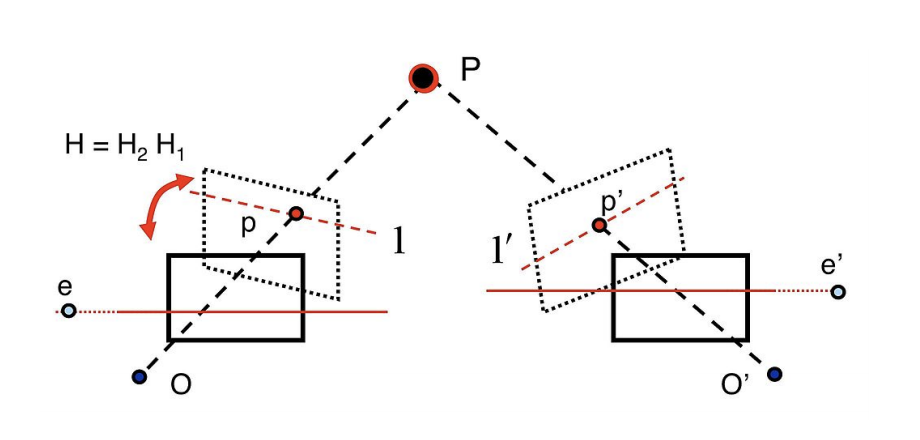
\includegraphics{image_rectification.png} Using the compute\_epipoles
function from the previous part and the given
compute\_matching\_homographies function, find the rectified images and
plot the parallel epipolar lines using the plot\_epipolar\_lines
function from above. You need to do this for both the matrix and the
warrior images. A sample output will look as below:
\includegraphics{sample_rectification.png}

    \begin{Verbatim}[commandchars=\\\{\}]
{\color{incolor}In [{\color{incolor}177}]:} \PY{k}{def} \PY{n+nf}{compute\PYZus{}matching\PYZus{}homographies}\PY{p}{(}\PY{n}{e2}\PY{p}{,} \PY{n}{F}\PY{p}{,} \PY{n}{im2}\PY{p}{,} \PY{n}{points1}\PY{p}{,} \PY{n}{points2}\PY{p}{)}\PY{p}{:}
              
              \PY{l+s+sd}{\PYZsq{}\PYZsq{}\PYZsq{}This function computes the homographies to get the rectified images}
          \PY{l+s+sd}{    input:}
          \PY{l+s+sd}{    e2\PYZhy{}\PYZhy{}\PYZgt{} epipole in image 2}
          \PY{l+s+sd}{    F\PYZhy{}\PYZhy{}\PYZgt{} the Fundamental matrix}
          \PY{l+s+sd}{    im2\PYZhy{}\PYZhy{}\PYZgt{} image2}
          \PY{l+s+sd}{    points1 \PYZhy{}\PYZhy{}\PYZgt{} corner points in image1}
          \PY{l+s+sd}{    points2\PYZhy{}\PYZhy{}\PYZgt{} corresponding corner points in image2}
          \PY{l+s+sd}{    output:}
          \PY{l+s+sd}{    H1\PYZhy{}\PYZhy{}\PYZgt{} Homography for image 1}
          \PY{l+s+sd}{    H2\PYZhy{}\PYZhy{}\PYZgt{} Homography for image 2}
          \PY{l+s+sd}{    \PYZsq{}\PYZsq{}\PYZsq{}}
              \PY{c+c1}{\PYZsh{} calculate H2}
              \PY{n}{width} \PY{o}{=} \PY{n}{im2}\PY{o}{.}\PY{n}{shape}\PY{p}{[}\PY{l+m+mi}{1}\PY{p}{]}
              \PY{n}{height} \PY{o}{=} \PY{n}{im2}\PY{o}{.}\PY{n}{shape}\PY{p}{[}\PY{l+m+mi}{0}\PY{p}{]}
          
              \PY{n}{T} \PY{o}{=} \PY{n}{np}\PY{o}{.}\PY{n}{identity}\PY{p}{(}\PY{l+m+mi}{3}\PY{p}{)}
              \PY{n}{T}\PY{p}{[}\PY{l+m+mi}{0}\PY{p}{]}\PY{p}{[}\PY{l+m+mi}{2}\PY{p}{]} \PY{o}{=} \PY{o}{\PYZhy{}}\PY{l+m+mf}{1.0} \PY{o}{*} \PY{n}{width} \PY{o}{/} \PY{l+m+mi}{2}
              \PY{n}{T}\PY{p}{[}\PY{l+m+mi}{1}\PY{p}{]}\PY{p}{[}\PY{l+m+mi}{2}\PY{p}{]} \PY{o}{=} \PY{o}{\PYZhy{}}\PY{l+m+mf}{1.0} \PY{o}{*} \PY{n}{height} \PY{o}{/} \PY{l+m+mi}{2}
          
              \PY{n}{e} \PY{o}{=} \PY{n}{T}\PY{o}{.}\PY{n}{dot}\PY{p}{(}\PY{n}{e2}\PY{p}{)}
              \PY{n}{e1\PYZus{}prime} \PY{o}{=} \PY{n}{e}\PY{p}{[}\PY{l+m+mi}{0}\PY{p}{]}
              \PY{n}{e2\PYZus{}prime} \PY{o}{=} \PY{n}{e}\PY{p}{[}\PY{l+m+mi}{1}\PY{p}{]}
              \PY{k}{if} \PY{n}{e1\PYZus{}prime} \PY{o}{\PYZgt{}}\PY{o}{=} \PY{l+m+mi}{0}\PY{p}{:}
                  \PY{n}{alpha} \PY{o}{=} \PY{l+m+mf}{1.0}
              \PY{k}{else}\PY{p}{:}
                  \PY{n}{alpha} \PY{o}{=} \PY{o}{\PYZhy{}}\PY{l+m+mf}{1.0}
          
              \PY{n}{R} \PY{o}{=} \PY{n}{np}\PY{o}{.}\PY{n}{identity}\PY{p}{(}\PY{l+m+mi}{3}\PY{p}{)}
              \PY{n}{R}\PY{p}{[}\PY{l+m+mi}{0}\PY{p}{]}\PY{p}{[}\PY{l+m+mi}{0}\PY{p}{]} \PY{o}{=} \PY{n}{alpha} \PY{o}{*} \PY{n}{e1\PYZus{}prime} \PY{o}{/} \PY{n}{np}\PY{o}{.}\PY{n}{sqrt}\PY{p}{(}\PY{n}{e1\PYZus{}prime}\PY{o}{*}\PY{o}{*}\PY{l+m+mi}{2} \PY{o}{+} \PY{n}{e2\PYZus{}prime}\PY{o}{*}\PY{o}{*}\PY{l+m+mi}{2}\PY{p}{)}
              \PY{n}{R}\PY{p}{[}\PY{l+m+mi}{0}\PY{p}{]}\PY{p}{[}\PY{l+m+mi}{1}\PY{p}{]} \PY{o}{=} \PY{n}{alpha} \PY{o}{*} \PY{n}{e2\PYZus{}prime} \PY{o}{/} \PY{n}{np}\PY{o}{.}\PY{n}{sqrt}\PY{p}{(}\PY{n}{e1\PYZus{}prime}\PY{o}{*}\PY{o}{*}\PY{l+m+mi}{2} \PY{o}{+} \PY{n}{e2\PYZus{}prime}\PY{o}{*}\PY{o}{*}\PY{l+m+mi}{2}\PY{p}{)}
              \PY{n}{R}\PY{p}{[}\PY{l+m+mi}{1}\PY{p}{]}\PY{p}{[}\PY{l+m+mi}{0}\PY{p}{]} \PY{o}{=} \PY{o}{\PYZhy{}} \PY{n}{alpha} \PY{o}{*} \PY{n}{e2\PYZus{}prime} \PY{o}{/} \PY{n}{np}\PY{o}{.}\PY{n}{sqrt}\PY{p}{(}\PY{n}{e1\PYZus{}prime}\PY{o}{*}\PY{o}{*}\PY{l+m+mi}{2} \PY{o}{+} \PY{n}{e2\PYZus{}prime}\PY{o}{*}\PY{o}{*}\PY{l+m+mi}{2}\PY{p}{)}
              \PY{n}{R}\PY{p}{[}\PY{l+m+mi}{1}\PY{p}{]}\PY{p}{[}\PY{l+m+mi}{1}\PY{p}{]} \PY{o}{=} \PY{n}{alpha} \PY{o}{*} \PY{n}{e1\PYZus{}prime} \PY{o}{/} \PY{n}{np}\PY{o}{.}\PY{n}{sqrt}\PY{p}{(}\PY{n}{e1\PYZus{}prime}\PY{o}{*}\PY{o}{*}\PY{l+m+mi}{2} \PY{o}{+} \PY{n}{e2\PYZus{}prime}\PY{o}{*}\PY{o}{*}\PY{l+m+mi}{2}\PY{p}{)}
          
              \PY{n}{f} \PY{o}{=} \PY{n}{R}\PY{o}{.}\PY{n}{dot}\PY{p}{(}\PY{n}{e}\PY{p}{)}\PY{p}{[}\PY{l+m+mi}{0}\PY{p}{]}
              \PY{n}{G} \PY{o}{=} \PY{n}{np}\PY{o}{.}\PY{n}{identity}\PY{p}{(}\PY{l+m+mi}{3}\PY{p}{)}
              \PY{n}{G}\PY{p}{[}\PY{l+m+mi}{2}\PY{p}{]}\PY{p}{[}\PY{l+m+mi}{0}\PY{p}{]} \PY{o}{=} \PY{o}{\PYZhy{}} \PY{l+m+mf}{1.0} \PY{o}{/} \PY{n}{f}
          
              \PY{n}{H2} \PY{o}{=} \PY{n}{np}\PY{o}{.}\PY{n}{linalg}\PY{o}{.}\PY{n}{inv}\PY{p}{(}\PY{n}{T}\PY{p}{)}\PY{o}{.}\PY{n}{dot}\PY{p}{(}\PY{n}{G}\PY{o}{.}\PY{n}{dot}\PY{p}{(}\PY{n}{R}\PY{o}{.}\PY{n}{dot}\PY{p}{(}\PY{n}{T}\PY{p}{)}\PY{p}{)}\PY{p}{)}
          
              \PY{c+c1}{\PYZsh{} calculate H1}
              \PY{n}{e\PYZus{}prime} \PY{o}{=} \PY{n}{np}\PY{o}{.}\PY{n}{zeros}\PY{p}{(}\PY{p}{(}\PY{l+m+mi}{3}\PY{p}{,} \PY{l+m+mi}{3}\PY{p}{)}\PY{p}{)}
              \PY{n}{e\PYZus{}prime}\PY{p}{[}\PY{l+m+mi}{0}\PY{p}{]}\PY{p}{[}\PY{l+m+mi}{1}\PY{p}{]} \PY{o}{=} \PY{o}{\PYZhy{}}\PY{n}{e2}\PY{p}{[}\PY{l+m+mi}{2}\PY{p}{]}
              \PY{n}{e\PYZus{}prime}\PY{p}{[}\PY{l+m+mi}{0}\PY{p}{]}\PY{p}{[}\PY{l+m+mi}{2}\PY{p}{]} \PY{o}{=} \PY{n}{e2}\PY{p}{[}\PY{l+m+mi}{1}\PY{p}{]}
              \PY{n}{e\PYZus{}prime}\PY{p}{[}\PY{l+m+mi}{1}\PY{p}{]}\PY{p}{[}\PY{l+m+mi}{0}\PY{p}{]} \PY{o}{=} \PY{n}{e2}\PY{p}{[}\PY{l+m+mi}{2}\PY{p}{]}
              \PY{n}{e\PYZus{}prime}\PY{p}{[}\PY{l+m+mi}{1}\PY{p}{]}\PY{p}{[}\PY{l+m+mi}{2}\PY{p}{]} \PY{o}{=} \PY{o}{\PYZhy{}}\PY{n}{e2}\PY{p}{[}\PY{l+m+mi}{0}\PY{p}{]}
              \PY{n}{e\PYZus{}prime}\PY{p}{[}\PY{l+m+mi}{2}\PY{p}{]}\PY{p}{[}\PY{l+m+mi}{0}\PY{p}{]} \PY{o}{=} \PY{o}{\PYZhy{}}\PY{n}{e2}\PY{p}{[}\PY{l+m+mi}{1}\PY{p}{]}
              \PY{n}{e\PYZus{}prime}\PY{p}{[}\PY{l+m+mi}{2}\PY{p}{]}\PY{p}{[}\PY{l+m+mi}{1}\PY{p}{]} \PY{o}{=} \PY{n}{e2}\PY{p}{[}\PY{l+m+mi}{0}\PY{p}{]}
          
              \PY{n}{v} \PY{o}{=} \PY{n}{np}\PY{o}{.}\PY{n}{array}\PY{p}{(}\PY{p}{[}\PY{l+m+mi}{1}\PY{p}{,} \PY{l+m+mi}{1}\PY{p}{,} \PY{l+m+mi}{1}\PY{p}{]}\PY{p}{)}
              \PY{n}{M} \PY{o}{=} \PY{n}{e\PYZus{}prime}\PY{o}{.}\PY{n}{dot}\PY{p}{(}\PY{n}{F}\PY{p}{)} \PY{o}{+} \PY{n}{np}\PY{o}{.}\PY{n}{outer}\PY{p}{(}\PY{n}{e2}\PY{p}{,} \PY{n}{v}\PY{p}{)}
          
              \PY{n}{points1\PYZus{}hat} \PY{o}{=} \PY{n}{H2}\PY{o}{.}\PY{n}{dot}\PY{p}{(}\PY{n}{M}\PY{o}{.}\PY{n}{dot}\PY{p}{(}\PY{n}{points1}\PY{p}{)}\PY{p}{)}\PY{o}{.}\PY{n}{T}
              \PY{n}{points2\PYZus{}hat} \PY{o}{=} \PY{n}{H2}\PY{o}{.}\PY{n}{dot}\PY{p}{(}\PY{n}{points2}\PY{p}{)}\PY{o}{.}\PY{n}{T}
          
              \PY{n}{W} \PY{o}{=} \PY{n}{points1\PYZus{}hat} \PY{o}{/} \PY{n}{points1\PYZus{}hat}\PY{p}{[}\PY{p}{:}\PY{p}{,} \PY{l+m+mi}{2}\PY{p}{]}\PY{o}{.}\PY{n}{reshape}\PY{p}{(}\PY{o}{\PYZhy{}}\PY{l+m+mi}{1}\PY{p}{,} \PY{l+m+mi}{1}\PY{p}{)}
              \PY{n}{b} \PY{o}{=} \PY{p}{(}\PY{n}{points2\PYZus{}hat} \PY{o}{/} \PY{n}{points2\PYZus{}hat}\PY{p}{[}\PY{p}{:}\PY{p}{,} \PY{l+m+mi}{2}\PY{p}{]}\PY{o}{.}\PY{n}{reshape}\PY{p}{(}\PY{o}{\PYZhy{}}\PY{l+m+mi}{1}\PY{p}{,} \PY{l+m+mi}{1}\PY{p}{)}\PY{p}{)}\PY{p}{[}\PY{p}{:}\PY{p}{,} \PY{l+m+mi}{0}\PY{p}{]}
          
              \PY{c+c1}{\PYZsh{} least square problem}
              \PY{n}{a1}\PY{p}{,} \PY{n}{a2}\PY{p}{,} \PY{n}{a3} \PY{o}{=} \PY{n}{np}\PY{o}{.}\PY{n}{linalg}\PY{o}{.}\PY{n}{lstsq}\PY{p}{(}\PY{n}{W}\PY{p}{,} \PY{n}{b}\PY{p}{)}\PY{p}{[}\PY{l+m+mi}{0}\PY{p}{]}
              \PY{n}{HA} \PY{o}{=} \PY{n}{np}\PY{o}{.}\PY{n}{identity}\PY{p}{(}\PY{l+m+mi}{3}\PY{p}{)}
              \PY{n}{HA}\PY{p}{[}\PY{l+m+mi}{0}\PY{p}{]} \PY{o}{=} \PY{n}{np}\PY{o}{.}\PY{n}{array}\PY{p}{(}\PY{p}{[}\PY{n}{a1}\PY{p}{,} \PY{n}{a2}\PY{p}{,} \PY{n}{a3}\PY{p}{]}\PY{p}{)}
          
              \PY{n}{H1} \PY{o}{=} \PY{n}{HA}\PY{o}{.}\PY{n}{dot}\PY{p}{(}\PY{n}{H2}\PY{p}{)}\PY{o}{.}\PY{n}{dot}\PY{p}{(}\PY{n}{M}\PY{p}{)}
              \PY{k}{return} \PY{n}{H1}\PY{p}{,} \PY{n}{H2}
\end{Verbatim}


    \begin{Verbatim}[commandchars=\\\{\}]
{\color{incolor}In [{\color{incolor}182}]:} \PY{c+c1}{\PYZsh{} convert points from euclidian to homogeneous}
          \PY{k}{def} \PY{n+nf}{to\PYZus{}homog}\PY{p}{(}\PY{n}{points}\PY{p}{)}\PY{p}{:}
              \PY{c+c1}{\PYZsh{} write your code here}
              \PY{n}{points\PYZus{}homog} \PY{o}{=} \PY{n}{np}\PY{o}{.}\PY{n}{vstack}\PY{p}{(}\PY{p}{(}\PY{n}{points}\PY{p}{,} \PY{n}{np}\PY{o}{.}\PY{n}{ones}\PY{p}{(}\PY{p}{(}\PY{l+m+mi}{1}\PY{p}{,} \PY{n}{points}\PY{o}{.}\PY{n}{shape}\PY{p}{[}\PY{l+m+mi}{1}\PY{p}{]}\PY{p}{)}\PY{p}{)}\PY{p}{)}\PY{p}{)}
              \PY{k}{return} \PY{n}{points\PYZus{}homog}
          
          
          \PY{c+c1}{\PYZsh{} convert points from homogeneous to euclidian}
          \PY{k}{def} \PY{n+nf}{from\PYZus{}homog}\PY{p}{(}\PY{n}{points\PYZus{}homog}\PY{p}{)}\PY{p}{:}
              \PY{c+c1}{\PYZsh{} write your code here}
              \PY{n}{points} \PY{o}{=} \PY{n}{points\PYZus{}homog}\PY{p}{[}\PY{p}{:}\PY{o}{\PYZhy{}}\PY{l+m+mi}{1}\PY{p}{,} \PY{p}{:}\PY{p}{]} \PY{o}{/} \PY{n}{points\PYZus{}homog}\PY{p}{[}\PY{o}{\PYZhy{}}\PY{l+m+mi}{1}\PY{p}{,} \PY{p}{:}\PY{p}{]}
              \PY{k}{return} \PY{n}{points}
          
          \PY{k}{def} \PY{n+nf}{warp2}\PY{p}{(}\PY{n}{source\PYZus{}img}\PY{p}{,} \PY{n}{target\PYZus{}size}\PY{p}{,} \PY{n}{offsetHW}\PY{p}{,} \PY{n}{H}\PY{p}{)}\PY{p}{:}
              \PY{c+c1}{\PYZsh{} Create a target image and select target points to create a homography from target image to source image,}
              \PY{c+c1}{\PYZsh{} in other words map each target point to a source point, and then create a warped version}
              \PY{c+c1}{\PYZsh{} of the image based on the homography by filling in the target image.}
              \PY{c+c1}{\PYZsh{} Make sure the new image (of size target\PYZus{}size) has the same number of color channels as source image}
              
              \PY{n}{x\PYZus{}coords} \PY{o}{=} \PY{p}{[}\PY{l+m+mi}{0}\PY{p}{,} \PY{n}{source\PYZus{}img}\PY{o}{.}\PY{n}{shape}\PY{p}{[}\PY{l+m+mi}{1}\PY{p}{]}\PY{p}{,} \PY{n}{source\PYZus{}img}\PY{o}{.}\PY{n}{shape}\PY{p}{[}\PY{l+m+mi}{1}\PY{p}{]}\PY{p}{,} \PY{l+m+mi}{0}\PY{p}{]} 
              \PY{n}{y\PYZus{}coords} \PY{o}{=} \PY{p}{[}\PY{l+m+mi}{0}\PY{p}{,} \PY{l+m+mi}{0}\PY{p}{,} \PY{n}{source\PYZus{}img}\PY{o}{.}\PY{n}{shape}\PY{p}{[}\PY{l+m+mi}{0}\PY{p}{]}\PY{p}{,} \PY{n}{source\PYZus{}img}\PY{o}{.}\PY{n}{shape}\PY{p}{[}\PY{l+m+mi}{0}\PY{p}{]}\PY{p}{]}
              \PY{n}{source\PYZus{}points} \PY{o}{=} \PY{n}{np}\PY{o}{.}\PY{n}{vstack}\PY{p}{(}\PY{p}{(}\PY{n}{x\PYZus{}coords}\PY{p}{,} \PY{n}{y\PYZus{}coords}\PY{p}{)}\PY{p}{)}
              
              \PY{n}{target\PYZus{}region} \PY{o}{=} \PY{n}{from\PYZus{}homog}\PY{p}{(}\PY{n}{np}\PY{o}{.}\PY{n}{dot}\PY{p}{(}\PY{n}{H}\PY{p}{,} \PY{n}{to\PYZus{}homog}\PY{p}{(}\PY{n}{source\PYZus{}points}\PY{p}{)}\PY{p}{)}\PY{p}{)}\PY{o}{.}\PY{n}{astype}\PY{p}{(}\PY{n+nb}{int}\PY{p}{)}
              \PY{n}{target\PYZus{}region}\PY{p}{[}\PY{l+m+mi}{0}\PY{p}{,} \PY{p}{:}\PY{p}{]} \PY{o}{=} \PY{n}{target\PYZus{}region}\PY{p}{[}\PY{l+m+mi}{0}\PY{p}{,} \PY{p}{:}\PY{p}{]} \PY{o}{+} \PY{n}{offsetHW}\PY{p}{[}\PY{l+m+mi}{1}\PY{p}{]} 
              \PY{n}{target\PYZus{}region}\PY{p}{[}\PY{l+m+mi}{1}\PY{p}{,} \PY{p}{:}\PY{p}{]} \PY{o}{=} \PY{n}{target\PYZus{}region}\PY{p}{[}\PY{l+m+mi}{1}\PY{p}{,} \PY{p}{:}\PY{p}{]} \PY{o}{+} \PY{n}{offsetHW}\PY{p}{[}\PY{l+m+mi}{0}\PY{p}{]} 
              
          
              \PY{n}{target\PYZus{}mask} \PY{o}{=} \PY{n}{np}\PY{o}{.}\PY{n}{ones}\PY{p}{(}\PY{n}{target\PYZus{}size}\PY{p}{)}
              
              \PY{n}{cv2}\PY{o}{.}\PY{n}{fillConvexPoly}\PY{p}{(}\PY{n}{target\PYZus{}mask}\PY{p}{,} \PY{n}{target\PYZus{}region}\PY{o}{.}\PY{n}{T}\PY{p}{,} \PY{l+m+mi}{1}\PY{p}{)}
              \PY{n}{target\PYZus{}mask} \PY{o}{=} \PY{n}{target\PYZus{}mask}\PY{o}{.}\PY{n}{astype}\PY{p}{(}\PY{n}{np}\PY{o}{.}\PY{n}{bool}\PY{p}{)}
              \PY{n}{row\PYZus{}y} \PY{o}{=} \PY{n}{np}\PY{o}{.}\PY{n}{linspace}\PY{p}{(}\PY{l+m+mi}{0}\PY{p}{,} \PY{n}{target\PYZus{}size}\PY{p}{[}\PY{l+m+mi}{0}\PY{p}{]}\PY{o}{\PYZhy{}}\PY{l+m+mi}{1}\PY{p}{,} \PY{n}{target\PYZus{}size}\PY{p}{[}\PY{l+m+mi}{0}\PY{p}{]}\PY{p}{)} \PY{c+c1}{\PYZsh{} 161}
              \PY{n}{col\PYZus{}x} \PY{o}{=} \PY{n}{np}\PY{o}{.}\PY{n}{linspace}\PY{p}{(}\PY{l+m+mi}{0}\PY{p}{,} \PY{n}{target\PYZus{}size}\PY{p}{[}\PY{l+m+mi}{1}\PY{p}{]}\PY{o}{\PYZhy{}}\PY{l+m+mi}{1}\PY{p}{,} \PY{n}{target\PYZus{}size}\PY{p}{[}\PY{l+m+mi}{1}\PY{p}{]}\PY{p}{)} \PY{c+c1}{\PYZsh{} 214}
              \PY{n}{col\PYZus{}idx}\PY{p}{,} \PY{n}{row\PYZus{}idx} \PY{o}{=} \PY{n}{np}\PY{o}{.}\PY{n}{meshgrid}\PY{p}{(}\PY{n}{col\PYZus{}x}\PY{p}{,} \PY{n}{row\PYZus{}y}\PY{p}{)} \PY{c+c1}{\PYZsh{} row 160, column 214}
              
              \PY{n}{target\PYZus{}mask} \PY{o}{=} \PY{n}{np}\PY{o}{.}\PY{n}{vstack}\PY{p}{(}\PY{p}{(}\PY{n}{col\PYZus{}idx}\PY{p}{[}\PY{n}{target\PYZus{}mask}\PY{p}{]}\PY{p}{,} \PY{n}{row\PYZus{}idx}\PY{p}{[}\PY{n}{target\PYZus{}mask}\PY{p}{]}\PY{p}{)}\PY{p}{)}\PY{o}{.}\PY{n}{astype}\PY{p}{(}\PY{n+nb}{int}\PY{p}{)} \PY{c+c1}{\PYZsh{} this is the index mask}
          
          
              \PY{n}{origin\PYZus{}target\PYZus{}mask} \PY{o}{=} \PY{n}{np}\PY{o}{.}\PY{n}{vstack}\PY{p}{(}\PY{p}{(}\PY{n}{target\PYZus{}mask}\PY{p}{[}\PY{l+m+mi}{0}\PY{p}{,} \PY{p}{:}\PY{p}{]} \PY{o}{\PYZhy{}} \PY{n}{offsetHW}\PY{p}{[}\PY{l+m+mi}{1}\PY{p}{]}\PY{p}{,} \PY{n}{target\PYZus{}mask}\PY{p}{[}\PY{l+m+mi}{1}\PY{p}{,} \PY{p}{:}\PY{p}{]} \PY{o}{\PYZhy{}} \PY{n}{offsetHW}\PY{p}{[}\PY{l+m+mi}{0}\PY{p}{]}\PY{p}{)}\PY{p}{)}
              \PY{n}{inv\PYZus{}H} \PY{o}{=} \PY{n}{np}\PY{o}{.}\PY{n}{linalg}\PY{o}{.}\PY{n}{inv}\PY{p}{(}\PY{n}{H}\PY{p}{)}
              
              \PY{n}{source\PYZus{}mask} \PY{o}{=} \PY{n}{from\PYZus{}homog}\PY{p}{(}\PY{n}{np}\PY{o}{.}\PY{n}{dot}\PY{p}{(}\PY{n}{inv\PYZus{}H}\PY{p}{,} \PY{n}{to\PYZus{}homog}\PY{p}{(}\PY{n}{origin\PYZus{}target\PYZus{}mask}\PY{p}{)}\PY{p}{)}\PY{p}{)}
              
              
              \PY{n}{mask\PYZus{}col} \PY{o}{=} \PY{p}{(}\PY{n}{source\PYZus{}mask}\PY{p}{[}\PY{l+m+mi}{0}\PY{p}{,} \PY{p}{:}\PY{p}{]}\PY{o}{\PYZlt{}}\PY{n}{source\PYZus{}img}\PY{o}{.}\PY{n}{shape}\PY{p}{[}\PY{l+m+mi}{1}\PY{p}{]}\PY{p}{)} \PY{o}{*} \PY{p}{(}\PY{n}{source\PYZus{}mask}\PY{p}{[}\PY{l+m+mi}{0}\PY{p}{,} \PY{p}{:}\PY{p}{]} \PY{o}{\PYZgt{}}\PY{o}{=} \PY{l+m+mi}{0}\PY{p}{)}
              \PY{n}{mask\PYZus{}row} \PY{o}{=} \PY{p}{(}\PY{n}{source\PYZus{}mask}\PY{p}{[}\PY{l+m+mi}{1}\PY{p}{,} \PY{p}{:}\PY{p}{]}\PY{o}{\PYZlt{}}\PY{n}{source\PYZus{}img}\PY{o}{.}\PY{n}{shape}\PY{p}{[}\PY{l+m+mi}{0}\PY{p}{]}\PY{p}{)} \PY{o}{*} \PY{p}{(}\PY{n}{source\PYZus{}mask}\PY{p}{[}\PY{l+m+mi}{1}\PY{p}{,} \PY{p}{:}\PY{p}{]} \PY{o}{\PYZgt{}}\PY{o}{=} \PY{l+m+mi}{0}\PY{p}{)}
              \PY{n}{mask} \PY{o}{=} \PY{n}{mask\PYZus{}row} \PY{o}{*} \PY{n}{mask\PYZus{}col}
              
              
              \PY{n}{target\PYZus{}mask\PYZus{}idx} \PY{o}{=} \PY{n}{target\PYZus{}mask}\PY{p}{[}\PY{p}{:}\PY{p}{,} \PY{n}{mask}\PY{p}{]}\PY{o}{.}\PY{n}{astype}\PY{p}{(}\PY{n+nb}{int}\PY{p}{)}
              \PY{n}{source\PYZus{}mask\PYZus{}idx} \PY{o}{=} \PY{n}{source\PYZus{}mask}\PY{p}{[}\PY{p}{:}\PY{p}{,} \PY{n}{mask}\PY{p}{]}\PY{o}{.}\PY{n}{astype}\PY{p}{(}\PY{n+nb}{int}\PY{p}{)}
              
              \PY{n}{target\PYZus{}img} \PY{o}{=} \PY{n}{np}\PY{o}{.}\PY{n}{ones}\PY{p}{(}\PY{n}{np}\PY{o}{.}\PY{n}{array}\PY{p}{(}\PY{n}{target\PYZus{}size}\PY{p}{)}\PY{o}{.}\PY{n}{astype}\PY{p}{(}\PY{n+nb}{int}\PY{p}{)}\PY{p}{)}
              
              \PY{n}{target\PYZus{}img}\PY{p}{[}\PY{n}{target\PYZus{}mask\PYZus{}idx}\PY{o}{.}\PY{n}{T}\PY{p}{[}\PY{p}{:}\PY{p}{,}\PY{l+m+mi}{1}\PY{p}{]}\PY{p}{,} \PY{n}{target\PYZus{}mask\PYZus{}idx}\PY{o}{.}\PY{n}{T}\PY{p}{[}\PY{p}{:}\PY{p}{,}\PY{l+m+mi}{0}\PY{p}{]}\PY{p}{]} \PYZbs{}
              \PY{o}{=} \PY{n}{source\PYZus{}img}\PY{p}{[}\PY{n}{source\PYZus{}mask\PYZus{}idx}\PY{o}{.}\PY{n}{T}\PY{p}{[}\PY{p}{:}\PY{p}{,}\PY{l+m+mi}{1}\PY{p}{]}\PY{p}{,} \PY{n}{source\PYZus{}mask\PYZus{}idx}\PY{o}{.}\PY{n}{T}\PY{p}{[}\PY{p}{:}\PY{p}{,}\PY{l+m+mi}{0}\PY{p}{]}\PY{p}{]}
              
              \PY{k}{return} \PY{n}{target\PYZus{}img}
          
          
          \PY{k}{def} \PY{n+nf}{getImageSize}\PY{p}{(}\PY{n}{im\PYZus{}maxHW}\PY{p}{,} \PY{n}{im\PYZus{}minHW}\PY{p}{)}\PY{p}{:}
              \PY{c+c1}{\PYZsh{} consider H}
              \PY{n}{offsetH} \PY{o}{=} \PY{o}{\PYZhy{}} \PY{n}{im\PYZus{}minHW}\PY{p}{[}\PY{l+m+mi}{0}\PY{p}{]}
              \PY{n}{offsetW} \PY{o}{=} \PY{o}{\PYZhy{}} \PY{n}{im\PYZus{}minHW}\PY{p}{[}\PY{l+m+mi}{1}\PY{p}{]}
              \PY{k}{if} \PY{n}{im\PYZus{}minHW}\PY{p}{[}\PY{l+m+mi}{0}\PY{p}{]} \PY{o}{\PYZlt{}} \PY{l+m+mi}{0}\PY{p}{:}
                  \PY{n}{height} \PY{o}{=} \PY{n}{im\PYZus{}maxHW}\PY{p}{[}\PY{l+m+mi}{0}\PY{p}{]} \PY{o}{\PYZhy{}} \PY{n}{im\PYZus{}minHW}\PY{p}{[}\PY{l+m+mi}{0}\PY{p}{]}
                  
              \PY{k}{else}\PY{p}{:}
                  \PY{n}{height} \PY{o}{=} \PY{n}{im\PYZus{}maxHW}\PY{p}{[}\PY{l+m+mi}{0}\PY{p}{]}
             
          
              \PY{k}{if} \PY{n}{im\PYZus{}minHW}\PY{p}{[}\PY{l+m+mi}{1}\PY{p}{]} \PY{o}{\PYZlt{}} \PY{l+m+mi}{0}\PY{p}{:}
                  \PY{n}{width} \PY{o}{=} \PY{n}{im\PYZus{}maxHW}\PY{p}{[}\PY{l+m+mi}{1}\PY{p}{]} \PY{o}{\PYZhy{}} \PY{n}{im\PYZus{}minHW}\PY{p}{[}\PY{l+m+mi}{1}\PY{p}{]}
              \PY{k}{else}\PY{p}{:}
                  \PY{n}{width} \PY{o}{=} \PY{n}{im\PYZus{}maxHW}\PY{p}{[}\PY{l+m+mi}{1}\PY{p}{]}
              \PY{k}{return} \PY{p}{(}\PY{n}{height}\PY{p}{,} \PY{n}{width}\PY{p}{)}\PY{p}{,} \PY{p}{(}\PY{n}{offsetH}\PY{p}{,} \PY{n}{offsetW}\PY{p}{)}
          
          
          
          \PY{k}{def} \PY{n+nf}{new\PYZus{}Wx\PYZus{}Hy}\PY{p}{(}\PY{n}{Wx}\PY{p}{,} \PY{n}{Hy}\PY{p}{,} \PY{n}{H}\PY{p}{)}\PY{p}{:}
              \PY{n}{x\PYZus{}coords} \PY{o}{=} \PY{p}{[}\PY{l+m+mi}{0}\PY{p}{,}\PY{n}{Wx}\PY{p}{,}\PY{l+m+mi}{0}\PY{p}{,}\PY{n}{Wx}\PY{p}{]} 
              \PY{n}{y\PYZus{}coords} \PY{o}{=} \PY{p}{[}\PY{l+m+mi}{0}\PY{p}{,}\PY{l+m+mi}{0}\PY{p}{,}\PY{n}{Hy}\PY{p}{,}\PY{n}{Hy}\PY{p}{]}
              \PY{n}{xy\PYZus{}coords} \PY{o}{=} \PY{n}{np}\PY{o}{.}\PY{n}{vstack}\PY{p}{(}\PY{p}{(}\PY{n}{x\PYZus{}coords}\PY{p}{,} \PY{n}{y\PYZus{}coords}\PY{p}{)}\PY{p}{)}
              \PY{n}{homog\PYZus{}xy\PYZus{}coords} \PY{o}{=} \PY{n}{to\PYZus{}homog}\PY{p}{(}\PY{n}{xy\PYZus{}coords}\PY{p}{)}
              
              \PY{n}{new\PYZus{}xy\PYZus{}coords} \PY{o}{=} \PY{n}{from\PYZus{}homog}\PY{p}{(}\PY{n}{H}\PY{o}{.}\PY{n}{dot}\PY{p}{(}\PY{n}{homog\PYZus{}xy\PYZus{}coords}\PY{p}{)}\PY{p}{)}
          
              \PY{n}{minH} \PY{o}{=} \PY{n}{np}\PY{o}{.}\PY{n}{floor}\PY{p}{(}\PY{n}{np}\PY{o}{.}\PY{n}{min}\PY{p}{(}\PY{n}{new\PYZus{}xy\PYZus{}coords}\PY{p}{[}\PY{l+m+mi}{1}\PY{p}{]}\PY{p}{)}\PY{p}{)}
              \PY{n}{minW} \PY{o}{=} \PY{n}{np}\PY{o}{.}\PY{n}{floor}\PY{p}{(}\PY{n}{np}\PY{o}{.}\PY{n}{min}\PY{p}{(}\PY{n}{new\PYZus{}xy\PYZus{}coords}\PY{p}{[}\PY{l+m+mi}{0}\PY{p}{]}\PY{p}{)}\PY{p}{)}
              
              \PY{n}{maxH} \PY{o}{=} \PY{n}{np}\PY{o}{.}\PY{n}{ceil}\PY{p}{(}\PY{n}{np}\PY{o}{.}\PY{n}{max}\PY{p}{(}\PY{n}{new\PYZus{}xy\PYZus{}coords}\PY{p}{[}\PY{l+m+mi}{1}\PY{p}{]}\PY{p}{)}\PY{p}{)}
              \PY{n}{maxW} \PY{o}{=} \PY{n}{np}\PY{o}{.}\PY{n}{ceil}\PY{p}{(}\PY{n}{np}\PY{o}{.}\PY{n}{max}\PY{p}{(}\PY{n}{new\PYZus{}xy\PYZus{}coords}\PY{p}{[}\PY{l+m+mi}{1}\PY{p}{]}\PY{p}{)}\PY{p}{)}
              \PY{k}{return} \PY{p}{(}\PY{n}{maxH}\PY{p}{,} \PY{n}{maxW}\PY{p}{)}\PY{p}{,} \PY{p}{(}\PY{n}{minH}\PY{p}{,} \PY{n}{minW}\PY{p}{)}
\end{Verbatim}


    \begin{Verbatim}[commandchars=\\\{\}]
{\color{incolor}In [{\color{incolor}183}]:} \PY{k}{def} \PY{n+nf}{image\PYZus{}rectification}\PY{p}{(}\PY{n}{im1}\PY{p}{,}\PY{n}{im2}\PY{p}{,}\PY{n}{points1}\PY{p}{,}\PY{n}{points2}\PY{p}{)}\PY{p}{:}
              \PY{l+s+sd}{\PYZsq{}\PYZsq{}\PYZsq{}this function provides the rectified images along with the new corner points as outputs for a given pair of }
          \PY{l+s+sd}{    images with corner correspondences}
          \PY{l+s+sd}{    input:}
          \PY{l+s+sd}{    im1\PYZhy{}\PYZhy{}\PYZgt{} image1}
          \PY{l+s+sd}{    im2\PYZhy{}\PYZhy{}\PYZgt{} image2}
          \PY{l+s+sd}{    points1\PYZhy{}\PYZhy{}\PYZgt{} corner points in image1 3*n}
          \PY{l+s+sd}{    points2\PYZhy{}\PYZhy{}\PYZgt{} corner points in image2}
          \PY{l+s+sd}{    outpu:}
          \PY{l+s+sd}{    rectified\PYZus{}im1\PYZhy{}\PYZhy{}\PYZgt{}rectified image 1}
          \PY{l+s+sd}{    rectified\PYZus{}im2\PYZhy{}\PYZhy{}\PYZgt{}rectified image 2}
          \PY{l+s+sd}{    new\PYZus{}cor1\PYZhy{}\PYZhy{}\PYZgt{} new corners in the rectified image 1}
          \PY{l+s+sd}{    new\PYZus{}cor2\PYZhy{}\PYZhy{}\PYZgt{} new corners in the rectified image 2}
          \PY{l+s+sd}{    \PYZsq{}\PYZsq{}\PYZsq{}}
              \PY{l+s+s2}{\PYZdq{}}\PY{l+s+s2}{your code here}\PY{l+s+s2}{\PYZdq{}}
              
              
              \PY{n}{F} \PY{o}{=} \PY{n}{fundamental\PYZus{}matrix}\PY{p}{(}\PY{n}{points1}\PY{p}{,} \PY{n}{points2}\PY{p}{)}
              \PY{n}{e1}\PY{p}{,} \PY{n}{e2} \PY{o}{=} \PY{n}{compute\PYZus{}epipole}\PY{p}{(}\PY{n}{F}\PY{p}{)}
              \PY{n}{H1}\PY{p}{,} \PY{n}{H2} \PY{o}{=} \PY{n}{compute\PYZus{}matching\PYZus{}homographies}\PY{p}{(}\PY{n}{e2}\PY{p}{,} \PY{n}{F}\PY{p}{,} \PY{n}{im2}\PY{p}{,} \PY{n}{points1}\PY{p}{,} \PY{n}{points2}\PY{p}{)}
             
              \PY{n}{im1\PYZus{}maxHW}\PY{p}{,} \PY{n}{im1\PYZus{}minHW} \PY{o}{=} \PY{n}{new\PYZus{}Wx\PYZus{}Hy}\PY{p}{(}\PY{n}{im1}\PY{o}{.}\PY{n}{shape}\PY{p}{[}\PY{l+m+mi}{1}\PY{p}{]}\PY{p}{,} \PY{n}{im1}\PY{o}{.}\PY{n}{shape}\PY{p}{[}\PY{l+m+mi}{0}\PY{p}{]}\PY{p}{,} \PY{n}{H1}\PY{p}{)}
              \PY{n}{im1\PYZus{}sizeHW}\PY{p}{,} \PY{n}{im1\PYZus{}offsetHW} \PY{o}{=} \PY{n}{getImageSize}\PY{p}{(}\PY{n}{im1\PYZus{}maxHW}\PY{p}{,} \PY{n}{im1\PYZus{}minHW}\PY{p}{)} \PY{c+c1}{\PYZsh{} height and width}
              
              \PY{n}{im2\PYZus{}maxHW}\PY{p}{,} \PY{n}{im2\PYZus{}minHW} \PY{o}{=} \PY{n}{new\PYZus{}Wx\PYZus{}Hy}\PY{p}{(}\PY{n}{im2}\PY{o}{.}\PY{n}{shape}\PY{p}{[}\PY{l+m+mi}{1}\PY{p}{]}\PY{p}{,} \PY{n}{im2}\PY{o}{.}\PY{n}{shape}\PY{p}{[}\PY{l+m+mi}{0}\PY{p}{]}\PY{p}{,} \PY{n}{H2}\PY{p}{)}
              \PY{n}{im2\PYZus{}sizeHW}\PY{p}{,} \PY{n}{im2\PYZus{}offsetHW} \PY{o}{=} \PY{n}{getImageSize}\PY{p}{(}\PY{n}{im2\PYZus{}maxHW}\PY{p}{,} \PY{n}{im2\PYZus{}minHW}\PY{p}{)} \PY{c+c1}{\PYZsh{} height and width}
              
          
              \PY{n}{img\PYZus{}sizeHW} \PY{o}{=} \PY{p}{(}\PY{n+nb}{int}\PY{p}{(}\PY{n+nb}{max}\PY{p}{(}\PY{n}{im2\PYZus{}sizeHW}\PY{p}{[}\PY{l+m+mi}{0}\PY{p}{]}\PY{p}{,} \PY{n}{im1\PYZus{}sizeHW}\PY{p}{[}\PY{l+m+mi}{0}\PY{p}{]}\PY{p}{)}\PY{p}{)}\PY{p}{,} \PY{n+nb}{int}\PY{p}{(}\PY{n+nb}{max}\PY{p}{(}\PY{n}{im2\PYZus{}sizeHW}\PY{p}{[}\PY{l+m+mi}{1}\PY{p}{]}\PY{p}{,} \PY{n}{im1\PYZus{}sizeHW}\PY{p}{[}\PY{l+m+mi}{1}\PY{p}{]}\PY{p}{)}\PY{p}{)}\PY{p}{)}
              
              \PY{n}{rectified\PYZus{}im1} \PY{o}{=} \PY{n}{warp2}\PY{p}{(}\PY{n}{im1}\PY{p}{,} \PY{n}{img\PYZus{}sizeHW}\PY{p}{,} \PY{n}{im1\PYZus{}offsetHW}\PY{p}{,} \PY{n}{H1}\PY{p}{)}
              \PY{n}{rectified\PYZus{}im2} \PY{o}{=} \PY{n}{warp2}\PY{p}{(}\PY{n}{im2}\PY{p}{,} \PY{n}{img\PYZus{}sizeHW}\PY{p}{,} \PY{n}{im2\PYZus{}offsetHW}\PY{p}{,} \PY{n}{H2}\PY{p}{)}
              
          
              \PY{n}{new\PYZus{}cor1} \PY{o}{=} \PY{n}{H1}\PY{o}{.}\PY{n}{dot}\PY{p}{(}\PY{n}{points1}\PY{p}{)}\PY{o}{/} \PY{n}{H1}\PY{o}{.}\PY{n}{dot}\PY{p}{(}\PY{n}{points1}\PY{p}{)}\PY{p}{[}\PY{o}{\PYZhy{}}\PY{l+m+mi}{1}\PY{p}{]} \PY{c+c1}{\PYZsh{} 3* N}
              \PY{n}{new\PYZus{}cor1}\PY{p}{[}\PY{l+m+mi}{0}\PY{p}{,} \PY{p}{:}\PY{p}{]} \PY{o}{=} \PY{n}{new\PYZus{}cor1}\PY{p}{[}\PY{l+m+mi}{0}\PY{p}{,} \PY{p}{:}\PY{p}{]} \PY{o}{+} \PY{n}{im1\PYZus{}offsetHW}\PY{p}{[}\PY{l+m+mi}{1}\PY{p}{]} 
              \PY{n}{new\PYZus{}cor1}\PY{p}{[}\PY{l+m+mi}{1}\PY{p}{,} \PY{p}{:}\PY{p}{]} \PY{o}{=} \PY{n}{new\PYZus{}cor1}\PY{p}{[}\PY{l+m+mi}{1}\PY{p}{,} \PY{p}{:}\PY{p}{]} \PY{o}{+} \PY{n}{im1\PYZus{}offsetHW}\PY{p}{[}\PY{l+m+mi}{0}\PY{p}{]} 
              
              \PY{n}{new\PYZus{}cor2} \PY{o}{=} \PY{n}{H2}\PY{o}{.}\PY{n}{dot}\PY{p}{(}\PY{n}{points2}\PY{p}{)}\PY{o}{/} \PY{n}{H2}\PY{o}{.}\PY{n}{dot}\PY{p}{(}\PY{n}{points2}\PY{p}{)}\PY{p}{[}\PY{o}{\PYZhy{}}\PY{l+m+mi}{1}\PY{p}{]}
              \PY{n}{new\PYZus{}cor2}\PY{p}{[}\PY{l+m+mi}{0}\PY{p}{,} \PY{p}{:}\PY{p}{]} \PY{o}{=} \PY{n}{new\PYZus{}cor2}\PY{p}{[}\PY{l+m+mi}{0}\PY{p}{,} \PY{p}{:}\PY{p}{]} \PY{o}{+} \PY{n}{im2\PYZus{}offsetHW}\PY{p}{[}\PY{l+m+mi}{1}\PY{p}{]} 
              \PY{n}{new\PYZus{}cor2}\PY{p}{[}\PY{l+m+mi}{1}\PY{p}{,} \PY{p}{:}\PY{p}{]} \PY{o}{=} \PY{n}{new\PYZus{}cor2}\PY{p}{[}\PY{l+m+mi}{1}\PY{p}{,} \PY{p}{:}\PY{p}{]} \PY{o}{+} \PY{n}{im2\PYZus{}offsetHW}\PY{p}{[}\PY{l+m+mi}{0}\PY{p}{]} 
              
              \PY{k}{return} \PY{n}{rectified\PYZus{}im1}\PY{p}{,} \PY{n}{rectified\PYZus{}im2}\PY{p}{,} \PY{n}{new\PYZus{}cor1}\PY{p}{,} \PY{n}{new\PYZus{}cor2}
\end{Verbatim}


    \hypertarget{matching-using-epipolar-geometry4-pts}{%
\subsubsection{Matching Using epipolar geometry{[}4
pts{]}}\label{matching-using-epipolar-geometry4-pts}}

We will now use the epipolar geometry constraint on the rectified images
and updated corner points to build a better matching algorithm. First,
detect 10 corners in Image1. Then, for each corner, do a linesearch
along the corresponding parallel epipolar line in Image2. Evaluate the
NCC score for each point along this line and return the best match (or
no match if all scores are below the NCCth). R is the radius (size) of
the NCC patch in the code below. You do not have to run this in both
directions. Show your result as in the naive matching part. Execute this
for the warrior and matrix images.

    \begin{Verbatim}[commandchars=\\\{\}]
{\color{incolor}In [{\color{incolor}192}]:} \PY{k}{def} \PY{n+nf}{display\PYZus{}correspondence}\PY{p}{(}\PY{n}{img1}\PY{p}{,} \PY{n}{img2}\PY{p}{,} \PY{n}{corrs}\PY{p}{)}\PY{p}{:}
              \PY{l+s+sd}{\PYZdq{}\PYZdq{}\PYZdq{}Plot matching result on image pair given images and correspondences}
          
          \PY{l+s+sd}{    Args:}
          \PY{l+s+sd}{        img1: Image 1.}
          \PY{l+s+sd}{        img2: Image 2.}
          \PY{l+s+sd}{        corrs: Corner correspondence}
          
          \PY{l+s+sd}{    \PYZdq{}\PYZdq{}\PYZdq{}}
              
              \PY{l+s+sd}{\PYZdq{}\PYZdq{}\PYZdq{}}
          \PY{l+s+sd}{    Your code here.}
          \PY{l+s+sd}{    You may refer to the show\PYZus{}matching\PYZus{}result function}
          \PY{l+s+sd}{    \PYZdq{}\PYZdq{}\PYZdq{}}
          \PY{c+c1}{\PYZsh{}     cor1 = to\PYZus{}homog(np.array([i[0] for i in corrs]).T)}
          \PY{c+c1}{\PYZsh{}     cor2 = to\PYZus{}homog(np.array([i[1] for i in corrs]).T)}
              
              \PY{n}{fig} \PY{o}{=} \PY{n}{plt}\PY{o}{.}\PY{n}{figure}\PY{p}{(}\PY{n}{figsize}\PY{o}{=}\PY{p}{(}\PY{l+m+mi}{8}\PY{p}{,} \PY{l+m+mi}{8}\PY{p}{)}\PY{p}{)}
              \PY{n}{plt}\PY{o}{.}\PY{n}{imshow}\PY{p}{(}\PY{n}{np}\PY{o}{.}\PY{n}{hstack}\PY{p}{(}\PY{p}{(}\PY{n}{img1}\PY{p}{,} \PY{n}{img2}\PY{p}{)}\PY{p}{)}\PY{p}{,} \PY{n}{cmap}\PY{o}{=}\PY{l+s+s1}{\PYZsq{}}\PY{l+s+s1}{gray}\PY{l+s+s1}{\PYZsq{}}\PY{p}{)} \PY{c+c1}{\PYZsh{} two dino images are of different sizes, resize one before use}
              \PY{k}{for} \PY{n}{p1}\PY{p}{,} \PY{n}{p2} \PY{o+ow}{in} \PY{n}{corrs}\PY{p}{:}
                  \PY{n}{plt}\PY{o}{.}\PY{n}{scatter}\PY{p}{(}\PY{n}{p1}\PY{p}{[}\PY{l+m+mi}{0}\PY{p}{]}\PY{p}{,} \PY{n}{p1}\PY{p}{[}\PY{l+m+mi}{1}\PY{p}{]}\PY{p}{,} \PY{n}{s}\PY{o}{=}\PY{l+m+mi}{35}\PY{p}{,} \PY{n}{edgecolors}\PY{o}{=}\PY{l+s+s1}{\PYZsq{}}\PY{l+s+s1}{r}\PY{l+s+s1}{\PYZsq{}}\PY{p}{,} \PY{n}{facecolors}\PY{o}{=}\PY{l+s+s1}{\PYZsq{}}\PY{l+s+s1}{none}\PY{l+s+s1}{\PYZsq{}}\PY{p}{)}
                  \PY{n}{plt}\PY{o}{.}\PY{n}{scatter}\PY{p}{(}\PY{n}{p2}\PY{p}{[}\PY{l+m+mi}{0}\PY{p}{]} \PY{o}{+} \PY{n}{img1}\PY{o}{.}\PY{n}{shape}\PY{p}{[}\PY{l+m+mi}{1}\PY{p}{]}\PY{p}{,} \PY{n}{p2}\PY{p}{[}\PY{l+m+mi}{1}\PY{p}{]}\PY{p}{,} \PY{n}{s}\PY{o}{=}\PY{l+m+mi}{35}\PY{p}{,} \PY{n}{edgecolors}\PY{o}{=}\PY{l+s+s1}{\PYZsq{}}\PY{l+s+s1}{r}\PY{l+s+s1}{\PYZsq{}}\PY{p}{,} \PY{n}{facecolors}\PY{o}{=}\PY{l+s+s1}{\PYZsq{}}\PY{l+s+s1}{none}\PY{l+s+s1}{\PYZsq{}}\PY{p}{)}
                  \PY{n}{plt}\PY{o}{.}\PY{n}{plot}\PY{p}{(}\PY{p}{[}\PY{n}{p1}\PY{p}{[}\PY{l+m+mi}{0}\PY{p}{]}\PY{p}{,} \PY{n}{p2}\PY{p}{[}\PY{l+m+mi}{0}\PY{p}{]} \PY{o}{+} \PY{n}{img1}\PY{o}{.}\PY{n}{shape}\PY{p}{[}\PY{l+m+mi}{1}\PY{p}{]}\PY{p}{]}\PY{p}{,} \PY{p}{[}\PY{n}{p1}\PY{p}{[}\PY{l+m+mi}{1}\PY{p}{]}\PY{p}{,} \PY{n}{p2}\PY{p}{[}\PY{l+m+mi}{1}\PY{p}{]}\PY{p}{]}\PY{p}{)}
             
              \PY{n}{plt}\PY{o}{.}\PY{n}{show}\PY{p}{(}\PY{p}{)}
          
              
          \PY{k}{def} \PY{n+nf}{correspondence\PYZus{}matching\PYZus{}epipole}\PY{p}{(}\PY{n}{img1}\PY{p}{,} \PY{n}{img2}\PY{p}{,} \PY{n}{corners1}\PY{p}{,} \PY{n}{F}\PY{p}{,} \PY{n}{R}\PY{p}{,} \PY{n}{NCCth}\PY{p}{)}\PY{p}{:}
              \PY{l+s+sd}{\PYZdq{}\PYZdq{}\PYZdq{}Find corner correspondence along epipolar line.}
          \PY{l+s+sd}{    Args:}
          \PY{l+s+sd}{        img1: Image 1.}
          \PY{l+s+sd}{        img2: Image 2.}
          \PY{l+s+sd}{        corners1: Detected corners in image 1.}
          \PY{l+s+sd}{        F: Fundamental matrix calculated using given ground truth corner correspondences.}
          \PY{l+s+sd}{        R: NCC matching window radius.}
          \PY{l+s+sd}{        NCCth: NCC matching threshold.}
          \PY{l+s+sd}{    }
          \PY{l+s+sd}{    Returns:}
          \PY{l+s+sd}{        Matching result to be used in display\PYZus{}correspondence function}
          
          \PY{l+s+sd}{    \PYZdq{}\PYZdq{}\PYZdq{}}
              \PY{l+s+sd}{\PYZdq{}\PYZdq{}\PYZdq{}}
          \PY{l+s+sd}{    Your code here.}
          \PY{l+s+sd}{    \PYZdq{}\PYZdq{}\PYZdq{}}
              
              \PY{n}{matching} \PY{o}{=} \PY{p}{[}\PY{p}{]}
              \PY{n}{num\PYZus{}corners1} \PY{o}{=} \PY{n}{corners1}\PY{o}{.}\PY{n}{shape}\PY{p}{[}\PY{l+m+mi}{0}\PY{p}{]} \PY{c+c1}{\PYZsh{} n * 2}
             
              \PY{n}{corners1\PYZus{}homog} \PY{o}{=} \PY{n}{np}\PY{o}{.}\PY{n}{hstack}\PY{p}{(}\PY{p}{(}\PY{n}{corners1}\PY{p}{,} \PY{n}{np}\PY{o}{.}\PY{n}{ones}\PY{p}{(}\PY{n}{num\PYZus{}corners1}\PY{p}{)}\PY{p}{[}\PY{p}{:}\PY{p}{,} \PY{k+kc}{None}\PY{p}{]}\PY{p}{)}\PY{p}{)}
              \PY{n}{lines2} \PY{o}{=} \PY{n}{np}\PY{o}{.}\PY{n}{dot}\PY{p}{(}\PY{n}{F}\PY{o}{.}\PY{n}{T}\PY{p}{,} \PY{n}{corners1\PYZus{}homog}\PY{o}{.}\PY{n}{T}\PY{p}{)} \PY{c+c1}{\PYZsh{} corners1 epipolar line in image2, lines2, 3*n}
          
              \PY{c+c1}{\PYZsh{} c1 is the center of corner 1}
              \PY{c+c1}{\PYZsh{} c2 is the center of corner 2}
              \PY{c+c1}{\PYZsh{} both in non homogeneous}
              \PY{k}{for} \PY{n}{i}\PY{p}{,} \PY{n}{c1} \PY{o+ow}{in} \PY{n+nb}{enumerate}\PY{p}{(}\PY{n}{corners1}\PY{p}{)}\PY{p}{:} 
                  \PY{n}{maximum} \PY{o}{=} \PY{o}{\PYZhy{}}\PY{l+m+mi}{100000000}
          
                  \PY{k}{for} \PY{n}{x\PYZus{}j} \PY{o+ow}{in} \PY{n+nb}{range}\PY{p}{(}\PY{n}{R}\PY{p}{,} \PY{n}{img2}\PY{o}{.}\PY{n}{shape}\PY{p}{[}\PY{l+m+mi}{1}\PY{p}{]} \PY{o}{\PYZhy{}} \PY{n}{R}\PY{p}{)}\PY{p}{:}
                      
                      \PY{n}{y\PYZus{}j} \PY{o}{=} \PY{n+nb}{int}\PY{p}{(}\PY{o}{\PYZhy{}}\PY{n}{lines2}\PY{p}{[}\PY{l+m+mi}{0}\PY{p}{]}\PY{p}{[}\PY{n}{i}\PY{p}{]}\PY{o}{/}\PY{n}{lines2}\PY{p}{[}\PY{l+m+mi}{1}\PY{p}{]}\PY{p}{[}\PY{n}{i}\PY{p}{]}\PY{o}{*} \PY{n}{x\PYZus{}j} \PY{o}{\PYZhy{}} \PY{n}{lines2}\PY{p}{[}\PY{l+m+mi}{2}\PY{p}{]}\PY{p}{[}\PY{n}{i}\PY{p}{]}\PY{o}{/}\PY{n}{lines2}\PY{p}{[}\PY{l+m+mi}{1}\PY{p}{]}\PY{p}{[}\PY{n}{i}\PY{p}{]}\PY{p}{)}
                      \PY{k}{if} \PY{n}{y\PYZus{}j} \PY{o}{\PYZgt{}}\PY{o}{=} \PY{n}{R} \PY{o+ow}{and} \PY{n}{y\PYZus{}j} \PY{o}{\PYZlt{}} \PY{n}{img2}\PY{o}{.}\PY{n}{shape}\PY{p}{[}\PY{l+m+mi}{0}\PY{p}{]}\PY{o}{\PYZhy{}}\PY{n}{R}\PY{p}{:}
                          \PY{n}{temp\PYZus{}c2} \PY{o}{=} \PY{n}{np}\PY{o}{.}\PY{n}{array}\PY{p}{(}\PY{p}{[}\PY{n}{x\PYZus{}j}\PY{p}{,} \PY{n}{y\PYZus{}j}\PY{p}{]}\PY{p}{)} \PY{c+c1}{\PYZsh{} non homogeneous}
                          \PY{n}{ncc\PYZus{}score} \PY{o}{=} \PY{n}{ncc\PYZus{}match}\PY{p}{(}\PY{n}{img1}\PY{p}{,} \PY{n}{img2}\PY{p}{,} \PY{n}{c1}\PY{p}{,} \PY{n}{temp\PYZus{}c2}\PY{p}{,} \PY{n}{R}\PY{p}{)}
                          \PY{k}{if} \PY{n}{ncc\PYZus{}score} \PY{o}{\PYZgt{}} \PY{n}{maximum}\PY{p}{:}
                              \PY{n}{maximum} \PY{o}{=} \PY{n}{ncc\PYZus{}score}
                              \PY{n}{best\PYZus{}c2} \PY{o}{=} \PY{n}{temp\PYZus{}c2}
                              
                  \PY{k}{if} \PY{n}{maximum} \PY{o}{\PYZgt{}} \PY{n}{NCCth}\PY{p}{:}
                      \PY{n}{matching}\PY{o}{.}\PY{n}{append}\PY{p}{(}\PY{p}{(}\PY{n}{c1}\PY{p}{,} \PY{n}{best\PYZus{}c2}\PY{p}{)}\PY{p}{)}
          
              \PY{k}{return} \PY{n}{matching}
\end{Verbatim}


    \begin{Verbatim}[commandchars=\\\{\}]
{\color{incolor}In [{\color{incolor}193}]:} \PY{n}{nCorners} \PY{o}{=} \PY{l+m+mi}{10} \PY{c+c1}{\PYZsh{} number of corners want to extract}
          \PY{c+c1}{\PYZsh{}decide the NCC matching window radius}
          \PY{n}{R} \PY{o}{=} \PY{l+m+mi}{5}
          \PY{n}{NCCth} \PY{o}{=} \PY{l+m+mf}{0.7}
          
          \PY{n}{I1}\PY{o}{=}\PY{n}{rgb2gray}\PY{p}{(}\PY{n}{imread}\PY{p}{(}\PY{l+s+s2}{\PYZdq{}}\PY{l+s+s2}{./p4/matrix/matrix0.png}\PY{l+s+s2}{\PYZdq{}}\PY{p}{)}\PY{p}{)}
          \PY{n}{I2}\PY{o}{=}\PY{n}{rgb2gray}\PY{p}{(}\PY{n}{imread}\PY{p}{(}\PY{l+s+s2}{\PYZdq{}}\PY{l+s+s2}{./p4/matrix/matrix1.png}\PY{l+s+s2}{\PYZdq{}}\PY{p}{)}\PY{p}{)}
          \PY{n}{cor1} \PY{o}{=} \PY{n}{np}\PY{o}{.}\PY{n}{load}\PY{p}{(}\PY{l+s+s2}{\PYZdq{}}\PY{l+s+s2}{./p4/dino/cor1.npy}\PY{l+s+s2}{\PYZdq{}}\PY{p}{)}
          \PY{n}{cor2} \PY{o}{=} \PY{n}{np}\PY{o}{.}\PY{n}{load}\PY{p}{(}\PY{l+s+s2}{\PYZdq{}}\PY{l+s+s2}{./p4/dino/cor2.npy}\PY{l+s+s2}{\PYZdq{}}\PY{p}{)}
          \PY{n}{I3}\PY{o}{=}\PY{n}{rgb2gray}\PY{p}{(}\PY{n}{imread}\PY{p}{(}\PY{l+s+s2}{\PYZdq{}}\PY{l+s+s2}{./p4/warrior/warrior0.png}\PY{l+s+s2}{\PYZdq{}}\PY{p}{)}\PY{p}{)}
          \PY{n}{I4}\PY{o}{=}\PY{n}{rgb2gray}\PY{p}{(}\PY{n}{imread}\PY{p}{(}\PY{l+s+s2}{\PYZdq{}}\PY{l+s+s2}{./p4/warrior/warrior1.png}\PY{l+s+s2}{\PYZdq{}}\PY{p}{)}\PY{p}{)}
          \PY{n}{cor3} \PY{o}{=} \PY{n}{np}\PY{o}{.}\PY{n}{load}\PY{p}{(}\PY{l+s+s2}{\PYZdq{}}\PY{l+s+s2}{./p4/warrior/cor1.npy}\PY{l+s+s2}{\PYZdq{}}\PY{p}{)}
          \PY{n}{cor4} \PY{o}{=} \PY{n}{np}\PY{o}{.}\PY{n}{load}\PY{p}{(}\PY{l+s+s2}{\PYZdq{}}\PY{l+s+s2}{./p4/warrior/cor2.npy}\PY{l+s+s2}{\PYZdq{}}\PY{p}{)}
          
          \PY{n}{rectified\PYZus{}im1}\PY{p}{,} \PY{n}{rectified\PYZus{}im2}\PY{p}{,} \PY{n}{new\PYZus{}cor1}\PY{p}{,} \PY{n}{new\PYZus{}cor2} \PY{o}{=} \PY{n}{image\PYZus{}rectification}\PY{p}{(}\PY{n}{I1}\PY{p}{,}\PY{n}{I2}\PY{p}{,}\PY{n}{cor1}\PY{p}{,}\PY{n}{cor2}\PY{p}{)}
          \PY{n}{rectified\PYZus{}im3}\PY{p}{,} \PY{n}{rectified\PYZus{}im4}\PY{p}{,} \PY{n}{new\PYZus{}cor3}\PY{p}{,} \PY{n}{new\PYZus{}cor4} \PY{o}{=} \PY{n}{image\PYZus{}rectification}\PY{p}{(}\PY{n}{I3}\PY{p}{,}\PY{n}{I4}\PY{p}{,}\PY{n}{cor3}\PY{p}{,}\PY{n}{cor4}\PY{p}{)}
          
          \PY{n}{F\PYZus{}new} \PY{o}{=} \PY{n}{fundamental\PYZus{}matrix}\PY{p}{(}\PY{n}{new\PYZus{}cor1}\PY{p}{,} \PY{n}{new\PYZus{}cor2}\PY{p}{)}
          \PY{c+c1}{\PYZsh{} detect corners using corner detector here, store in corners1}
          \PY{n}{corners1} \PY{o}{=} \PY{n}{corner\PYZus{}detect}\PY{p}{(}\PY{n}{rectified\PYZus{}im1}\PY{p}{,} \PY{n}{nCorners}\PY{p}{,} \PY{n}{smoothSTD}\PY{p}{,} \PY{n}{windowSize}\PY{p}{)}
          \PY{n}{corrs} \PY{o}{=} \PY{n}{correspondence\PYZus{}matching\PYZus{}epipole}\PY{p}{(}\PY{n}{rectified\PYZus{}im1}\PY{p}{,} \PY{n}{rectified\PYZus{}im2}\PY{p}{,} \PY{n}{corners1}\PY{p}{,} \PY{n}{F\PYZus{}new}\PY{p}{,} \PY{n}{R}\PY{p}{,} \PY{n}{NCCth}\PY{p}{)}
          \PY{n}{display\PYZus{}correspondence}\PY{p}{(}\PY{n}{rectified\PYZus{}im1}\PY{p}{,} \PY{n}{rectified\PYZus{}im2}\PY{p}{,} \PY{n}{corrs}\PY{p}{)}
          
          \PY{n}{F\PYZus{}new2} \PY{o}{=} \PY{n}{fundamental\PYZus{}matrix}\PY{p}{(}\PY{n}{new\PYZus{}cor3}\PY{p}{,} \PY{n}{new\PYZus{}cor4}\PY{p}{)}
          \PY{c+c1}{\PYZsh{} detect corners using corner detector here, store in corners2}
          \PY{n}{corners2} \PY{o}{=} \PY{n}{corner\PYZus{}detect}\PY{p}{(}\PY{n}{rectified\PYZus{}im3}\PY{p}{,} \PY{n}{nCorners}\PY{p}{,} \PY{n}{smoothSTD}\PY{p}{,} \PY{n}{windowSize}\PY{p}{)}
          \PY{n}{corrs} \PY{o}{=} \PY{n}{correspondence\PYZus{}matching\PYZus{}epipole}\PY{p}{(}\PY{n}{rectified\PYZus{}im3}\PY{p}{,} \PY{n}{rectified\PYZus{}im4}\PY{p}{,} \PY{n}{corners2}\PY{p}{,} \PY{n}{F\PYZus{}new2}\PY{p}{,} \PY{n}{R}\PY{p}{,} \PY{n}{NCCth}\PY{p}{)}
          \PY{n}{display\PYZus{}correspondence}\PY{p}{(}\PY{n}{rectified\PYZus{}im3}\PY{p}{,} \PY{n}{rectified\PYZus{}im4}\PY{p}{,} \PY{n}{corrs}\PY{p}{)}
\end{Verbatim}


    \begin{Verbatim}[commandchars=\\\{\}]
/usr/local/lib/python3.7/site-packages/ipykernel\_launcher.py:6: DeprecationWarning: `imread` is deprecated!
`imread` is deprecated in SciPy 1.0.0, and will be removed in 1.2.0.
Use ``imageio.imread`` instead.
  
/usr/local/lib/python3.7/site-packages/ipykernel\_launcher.py:7: DeprecationWarning: `imread` is deprecated!
`imread` is deprecated in SciPy 1.0.0, and will be removed in 1.2.0.
Use ``imageio.imread`` instead.
  import sys
/usr/local/lib/python3.7/site-packages/ipykernel\_launcher.py:10: DeprecationWarning: `imread` is deprecated!
`imread` is deprecated in SciPy 1.0.0, and will be removed in 1.2.0.
Use ``imageio.imread`` instead.
  \# Remove the CWD from sys.path while we load stuff.
/usr/local/lib/python3.7/site-packages/ipykernel\_launcher.py:11: DeprecationWarning: `imread` is deprecated!
`imread` is deprecated in SciPy 1.0.0, and will be removed in 1.2.0.
Use ``imageio.imread`` instead.
  \# This is added back by InteractiveShellApp.init\_path()
/usr/local/lib/python3.7/site-packages/ipykernel\_launcher.py:61: FutureWarning: `rcond` parameter will change to the default of machine precision times ``max(M, N)`` where M and N are the input matrix dimensions.
To use the future default and silence this warning we advise to pass `rcond=None`, to keep using the old, explicitly pass `rcond=-1`.
/usr/local/lib/python3.7/site-packages/ipykernel\_launcher.py:29: RuntimeWarning: invalid value encountered in true\_divide

    \end{Verbatim}

    \begin{center}
    \adjustimage{max size={0.9\linewidth}{0.9\paperheight}}{output_31_1.png}
    \end{center}
    { \hspace*{\fill} \\}
    
    \begin{center}
    \adjustimage{max size={0.9\linewidth}{0.9\paperheight}}{output_31_2.png}
    \end{center}
    { \hspace*{\fill} \\}
    

    % Add a bibliography block to the postdoc
    
    
    
    \end{document}
